\documentclass[a4paper, 11pt, oneside, openright, english]{memoir}
\usepackage{booktabs}
\usepackage[table,xcdraw,dvipsnames]{xcolor}
\usepackage{xcolor}
\definecolor{poliblu}{RGB}{184, 200, 213}
\usepackage{multirow}
\usepackage{style/style}
\usepackage[super]{nth}
\usepackage{longtable}
\usepackage{graphicx,subfig}
\usepackage{listings}
\usepackage{hyperref} % provides \url{}
\usepackage{style/alloy}
\usepackage{ragged2e}

\newcommand{\usecase}[8]{
    \def\arraystretch{1.5} % This adds padding to table rows (and more)
    \subsubsection*{UC.#1: #2}
    \vspace*{0.1cm}
    \begin{center}
     \begin{tabular}{|l|p{12cm}|}
         \hline
         \textbf{Actor(s)} & #3 \\
         \hline
         \textbf{Entry Condition} & #4 \\
         \hline
         \textbf{Event Flow} & #5 \\
         \hline
         \textbf{Exit Condition} & #6 \\
         \hline
          \textbf{Exceptions} & #7 \\
         \hline
         \textbf{Notes} & #8 \\
         \hline
      \end{tabular}
    \end{center}
}

\begin{document}
	\begin{titlingpage}
	\begin{center}
		
\includegraphics[width=0.4\textwidth]{logo}
		
		\vspace{0.25cm}
		
		\LARGE POLITECNICO DI MILANO\\
		
		\vspace{0.2cm}
		
		\Large Computer Science and Engineering
		
		\vspace{0.8cm}
	
		\Huge \textbf{Design Document}
		
		\vspace{0.5cm}
		\huge CodeKataBattle
		
		\vspace{1.5cm}
		\LARGE Software Engineering 2 Project\\
		\Large Academic year 2023 - 2024\\
		\vspace{1cm}
		3 January 2024\\Version 1.0
		\vspace{2.5cm}
		
		\large
		\begin{minipage}{.1\textwidth}
			\null
		\end{minipage}%
		\begin{minipage}{.4\textwidth}
			\textit{Authors}:\\
			Massara Gianluca\\
			Nguyen Ba Chiara Thien Thao\\
			Nicotri Flavia
		\end{minipage}%
		\begin{minipage}{.4\textwidth}
			\raggedleft	
			\textit{Professor}:\\
			Matteo Giovanni Rossi\\
			\phantom{placeholder}
		\end{minipage}%
		\begin{minipage}{.1\textwidth}
			\null
		\end{minipage}
	
			
		\end{center}
\end{titlingpage}
    \include{intro/version_history}
	\pagenumbering{Roman}

	\tableofcontents
	\pagenumbering{arabic}
	\chapter{Introduction}

\section{Purpose}
In the last years, more and more students are becoming interested in programming and many educators have realised 
the need of new innovative methods to improve coding skills. \\
CodeKataBattle aims to assist students in enhancing their programming skills by challenging them with creative tasks
 in a competitive and stimulating environment. \\
 \\
 The following document wants to describe the system focusing on the requirements and specifications, providing scenarios 
 and use cases to specify what the system must do and how it should interact with the stakeholders.\\  

 \subsection{Goals}
 In the following table we describe the main goals that our system wants to achive.\\
 \begin{table}[H]
    \centering
    \resizebox{0.8\textwidth}{!}{%
    \begin{tabular}{|c|l|}
    \hline
    \rowcolor[HTML]{b8c8d5}
    \multicolumn{1}{|c|}{\cellcolor[HTML]{b8c8d5}\textbf{Goal}} & \multicolumn{1}{c|}{\cellcolor[HTML]{b8c8d5}\textbf{Description}} \\ \hline
    G.1 \label{G.1}& \begin{tabular}[c]{@{}l@{}} Allow students to compete in a tournament \end{tabular}  \\ \hline
    G.2 \label{G.2}& Allow educators to create challenges for students. \\ \hline
    G.3 \label{G.3}& Allow educators to grade students' projects. \\ \hline
    G.4 \label{G.4}& Allow students to collect badges. \\ \hline
    \end{tabular}
    }
    \end{table}
    \clearpage
\section{Scope}
The main actors of the system are students and educators. Educators can:
\begin{itemize}
    \item \textbf{Create a tournament:} decide which colleagues can create battles within the tournament and define badges 
    that represent the achievements of individual students; 
    \item \textbf{Create a battle:} set configurations and rules for that battle;
    \item \textbf{Evaluate:} manually assign a personal score to the students' works.
\end{itemize}

Students can:
\begin{itemize}
    \item \textbf{Join a tournament};
    \item \textbf{Partecipate in a battle:} create a team and complete the project with his code;
    \item \textbf{Collect badges} based on the rules of the tournament and his performance.
\end{itemize}

\subsection{World Phenomena}

\begin{table}[H]
    \centering
    \resizebox{0.8\textwidth}{!}{%
    \begin{tabular}{|c|l|}
    \hline
    \rowcolor[HTML]{b8c8d5}
    \multicolumn{1}{|c|}{\cellcolor[HTML]{b8c8d5}\textbf{W.P.}} & \multicolumn{1}{c|}{\cellcolor[HTML]{b8c8d5}\textbf{Description}} \\ \hline
    WP.1 \label{WP.1}& An educator wants to create a tournament.  \\ \hline
    WP.2 \label{WP.2}& An educator wants to create a new battle. \\ \hline
    WP.3 \label{WP.3}& A student wants to join a tournament.   \\ \hline
    WP.4 \label{WP.4}& A student wants to join a battle.  \\ \hline
    WP.5 \label{WP.5}& An educator evaluates the works done by students.   \\ \hline
    \end{tabular}
    }
    \end{table}
    \clearpage

\subsection{Shared Phenomena}

\begin{table}[H]
    \centering
    \resizebox{\textwidth}{!}{%
    \begin{tabular}{|c|l|c|}
    \hline
    \rowcolor[HTML]{b8c8d5}
    \multicolumn{1}{|c|}{\cellcolor[HTML]{b8c8d5}\textbf{S.P.}} & \multicolumn{1}{c|}{\cellcolor[HTML]{b8c8d5}\textbf{Description}}& \multicolumn{1}{c|}{\cellcolor[HTML]{b8c8d5}\textbf{Controlled by}} \\ \hline
    SP.1 \label{SP.1}&  The system notifies the student about upcoming battles. & Machine \\ \hline
    SP.2 \label{SP.2}&  The student commits his code. & World  \\ \hline
    SP.3 \label{SP.3}&  The educator configures the tournament rules. & World   \\ \hline
    SP.4 \label{SP.4}&  The student forms a team. & World   \\ \hline
    SP.5 \label{SP.5}&  \begin{tabular}[c]{@{}l@{}} The educator grants other colleagues the permission to \\create battles within a tournament. \end{tabular} & World  \\ \hline
    SP.6 \label{SP.6}&  The educator configures the battle. & World  \\ \hline
    SP.7 \label{SP.7}&  The student joins a team. & World  \\ \hline
    SP.8 \label{SP.8}&  The system creates a GitHub repository. & Machine  \\ \hline
    SP.9 \label{SP.9}&  The student forks and sets up the GitHub repository. & World  \\ \hline
    SP.10 \label{SP.10}&  GitHub Actions notifies the system about students' commits. & World  \\ \hline
    SP.11 \label{SP.11}&  The system shows the battle score of the team. & Machine  \\ \hline
    SP.12 \label{SP.12}&  The system notifies when the final battle rank becomes available. & Machine  \\ \hline
    SP.13 \label{SP.13}&  The system shows the tournament rank. & Machine  \\ \hline
    SP.14 \label{SP.14}&  The system shows the list of ongoing tournaments. & Machine  \\ \hline
    SP.15 \label{SP.15}&  The system shows the student's badges. & Machine  \\ \hline
    SP.16 \label{SP.16}&  The educator defines the badges of a tournament. & World  \\ \hline
    SP.17 \label{SP.17}&  All users can visualize the profile of a user. & World  \\ \hline
    \end{tabular}
    }
    \end{table}
    \clearpage


\section{Definitions, Acronyms, Abbreviations}
\subsection{Definitions}
\begin{table}[H]
    \centering
    \begin{tabular}{|c|l|}
    \hline
    \rowcolor[HTML]{B8C8D5} 
    \textbf{Definitions} & \multicolumn{1}{c|}{\cellcolor[HTML]{B8C8D5}\textbf{Meaning}} \\ \hline
    Code Kata & \begin{tabular}[c]{@{}l@{}}A code kata battle is a programming exercise in a programming language \\
        of choice. The exercise includes a brief textual description and a software \\
        project with build automation scripts that contains a set of test cases that the \\
        program must pass, but without the program implementation. \end{tabular}  \\ \hline
    \end{tabular}
\end{table}


\subsection{Acronyms}

\begin{table}[H]
    \centering
    \begin{tabular}{|c|l|}
    \hline
    \rowcolor[HTML]{B8C8D5} 
    \textbf{Acronyms} & \multicolumn{1}{c|}{\cellcolor[HTML]{B8C8D5}\textbf{Meaning}} \\ \hline
    CKB & CodeKataBattle  \\ \hline
    \end{tabular}
\end{table}

\subsection{Abbreviations}

\begin{table}[H]
    \centering
    \begin{tabular}{|c|l|}
    \hline
    \rowcolor[HTML]{B8C8D5} 
    \textbf{Abbreviations} & \multicolumn{1}{c|}{\cellcolor[HTML]{B8C8D5}\textbf{Meaning}} \\ \hline
    WP & World Phenomena  \\ \hline
    SP & Shared Phenomena \\ \hline
    G  & Goal             \\ \hline
    R  & Requirement             \\ \hline
    UC  & Use Case             \\ \hline
    NFR  & Non Functional Requirement             \\ \hline
    D  & Domain Assumption             \\ \hline
    w.r.t. & with reference to \\ \hline
    e.g. & exempli gratia \\ \hline
    i.e. & id est \\ \hline
    etc. & etcetera \\ \hline
    \end{tabular}
\end{table}

\section{Revision History}

\section{Reference Documents}
\begin{itemize}
    \item Course slides on WeBeep. 
    \item RASD assignment document.
\end{itemize}


\section{Document Structure}
The structure of this RASD document is the following:
\begin{enumerate}
    \item \textbf{Introduction}: In this chapter the purpose of this document is presented highlighting in particular the main goals, 
    the audience which is referred to, the identification of the product and application domain  describing world and shared phenomena and, 
    lastly, the terms definitions.
    \item \textbf{Overall Description}: This chapter describes the possible scenarios of the platform, the shared phenomena presented at the 
    beginning of the document and assumptions on the domain of the application.
    \item \textbf{Specific Requirements}: This chapter includes all the requirements in a more specific way than the "Overall Description" section. 
    Moreover, it is useful to show functional requirements in terms of use cases diagrams, sequence/activity diagrams.
    \item \textbf{Formal Analysis Using Alloy}: This chapter includes Alloy models which are used for the description of the application domain and 
    his properties, referring to the operations which the system must provide.
    \item \textbf{Effort Spent}: This chapter shows the effort spent in terms of time for each team member and the whole team.
    \item \textbf{References}: This chapter includes all documents that were helpful in drafting the RASD.
\end{enumerate}
	\chapter{Overall Description}

\section{Product perspective}
In this section we analyze a list of real 
scenariosand diagrams illustrating further details about shared phenomenas.\\

\subsection{Scenarios}
\begin{enumerate}
    \item \textbf{Registration} \\
    Prof. White reads about CodeKataBattle in a online spot and decides to use the platform to 
    challenge his students. So, he creates an account using his email address and personal information 
    and convinces his colleagues to join the platform.\\
    Alice and her classmates, after prof. White's lesson, are interested in improving their coding 
    skills and sign up to CKB. Alice provides her email address and personal information; after the email 
    confimation goes well, 
    she can complete the registration process by linking her CKB account to her GitHub account. Her nickname 
    on the platform will be her GitHub one.\\
    After the registration, both Prof. White and Alice can visualize the profile of all the other 
    students and the information about the ongoing tournaments.

    \item \textbf{Creation of tournaments} \\
    Prof. Brown and prof. Smith want to decide whose class is better at programming. So Prof.Brown 
    create a tournament on CKB and invite his colleague to create battles within the tournament. Prof. Brown 
    sets a deadline by which their students can subscribe. A notification is sent to all CKB students. \\
    
    \item \textbf{Creation of battles} \\
    Prof. Bloom has been granted the permission to create battles in a tournament, so he uploads a 
    code kata battle. First he writes a brief textual description of the exercise, then he includes 
    the software project with build automation scripts and test cases. He also sets some rules: 
    minimum and maximum number of students per group, registration deadline, final submission deadline, 
    automated evaluation parameters.\\
    Finally, he chooses to include some optional manual evaluation of his students' work.\\

    \item \textbf{Students join a battle} \\
    Bob registered to the CKB platform and received a notification about an interesting tournament 
    and he subscribed to it. \\
    He is notified about a new interesting battle in that tournament is upcoming. Before the registration 
    deadline expires, Bob can form a group, so invites his girlfriend Eva to join him. After the registration 
    deadline ends, they are sent the link of the GitHub repository of the code kata. To be able to start 
    working on the project, Bob and Eva must fork the repository and set up an automated workflow through 
    GitHub Actions to inform the CKB platform about their commits.\\

    \item \textbf{Upload of a solution} \\
    Charlie has joined a battle with his friends and thinks that they have found a good solution to 
    the assigned problem. So he push his code before the final deadline to the main branch of their 
    repository. \\This battle doesn't expect any manual evaluation by the educator, so as soon as 
    push the solution, the platform evaluates it and they can visualize their updated battle score. 
    After the final deadline has expired, Charlie can also see the current tournament ranking. \\

    \item \textbf{Evaluation of project}\\
    When Prof. Cooper created the battle, he decided to include manual evaluation in the battle rules: 
    he wants the system to assign up to 75 points, while he will assign the remaing 25 points. 
    So, scores will always be between 0 and 100.\\
    After the final deadline, prof. Cooper can see all the groups' work and he evaluates them according 
    to some personal parameters such that design quality, code cleanliness, compliance with specifications.\\

    \item \textbf{Creation of gamification badges}\\
    Prof. Moore has created a tournament and to spice things up he decides to include badges. 
    These are awarded according to the rules specific by him at tournament set up time: in particular, 
    he wants to reward the student with most commits and the student who have attended the most battles.\\
    The badges are assigned at the end of the tournament and the collected badges can be seen by everyone 
    visiting the student's profile. \\
\end{enumerate}

\subsection{Class diagrams}

\subsection{State diagrams}

\section{Product functions}
\subsection{Sign up and login}
These functions are available to both students and educators.\\
The sign up functionality allows users to register on the platform: in particular, each user will provide an email 
and a password. Then a verification email is sent to the user.
After the confirmation, the user must provide their personal information (name, surname, date of birth) and 
if the user is a student they are required to provide a GitHub account.\\
Once registered, both students and educators can visualize the profile of all the other users.\\
The login functionality allows users to access the platform using their email and password.\\

\subsection{Creation of a tournament}
Educators can create tournaments, programming competitions composed of various code kata battles.\\
The creator of the tournament can invite other educators and grant them the permission to create battles within the 
context of the tournament.\\
When they create a tournament, educators sets a registration deadline and can also define badges, i.e., awards that 
represent particular achievements of individual students: the educator may use pre-defined variables and rules or create 
new ones. Badges are awarded automatically at the end of a tournament.\\
Information about ongoing tournaments is avalaible to all subscribed users.\\

\subsection{Creation of a battle}
After being granted such permission from the creator of the tournament, educators can create code kata battles within the
context of the tournament.\\
A code kata battle is a programming exercise in a programming language chosen by its creator. It includes a textual description
of the exercise and a software project with build automation scripts and test cases.\\
To create a battle, the educator must upload the code kata, set the rules regarding groups composition (minimum and maximum 
number of members), set a registration deadline, set a final submission deadline, and set evaluation parameters. They may also 
specify if they want to include a manual evaluation of the students' work, in addition the mandatory automated one, after the 
submission deadline expires.\\
Educators can see the current battle ranking evolve during the battle.\\

\subsection{Join a tournament}
Students can join any tournament before its registration deadline expires. By signing up to a tournament, they also 
subscribe to notifications regarding upcoming battles within the context of that tournament.\\
Students also receive a notification when the tournament ends.\\
By participating in a tournament, students can earn badges that can be visualized in their profile.\\

\subsection{Join a battle}
Students subscribed to a tournament can join any upcoming battle before its registration deadline expires.\\
Students can participate alone or in groups to the battle, according to the rules set for that battle by its creator.\\
When the registration deadline expires, students are sent an email with the link of the GitHub repository containing the 
code kata. To start working on the project, they are required to fork the repository and set up an automated workflow, 
using GitHub Actions, to inform CKB about new commits into the main branch of their repository.\\
As soon as students push a solution it is automatically evaluated, so they can see their current battle score and their 
battle rank.\\
When the submission deadline (and, if required, the manual evaluation stage) ends, students are notified about their final 
battle score and rank and they can see their updated tournament score.\\

\subsection{Evaluation of a project}
According to the parameters set by the creator of the battle, the system automatically evaluates the students' work with regard to
\begin{enumerate}
  \item functional aspects (i.e., the percentage of passed test cases);
  \item timeliness (i.e., the time passed between the registration deadline and the last commit);
  \item code quality (extracted using static analysis tools).
\end{enumerate}
If the educator has decided to include manual evaluation in the battle rules, they can see all the groups' work and evaluate 
the students' work according to some personal parameters such that design quality, code cleanliness, compliance with specifications.\\
The final score is a natural number between 0 and 100 calculated as specified at battle creation time.\\


\section{User characteristics}

\section{Assumptions, dependecies and constraints}


	\chapter{Specific Requirements}

\section{External Interface Requirements}
In this section details about user interfaces, 
hardware and application programming interfaces are described.

\subsection{User Interfaces}
In this subsection we present user interfaces for both types of users, educators and students.

\begin{figure}[H]
    \centering
    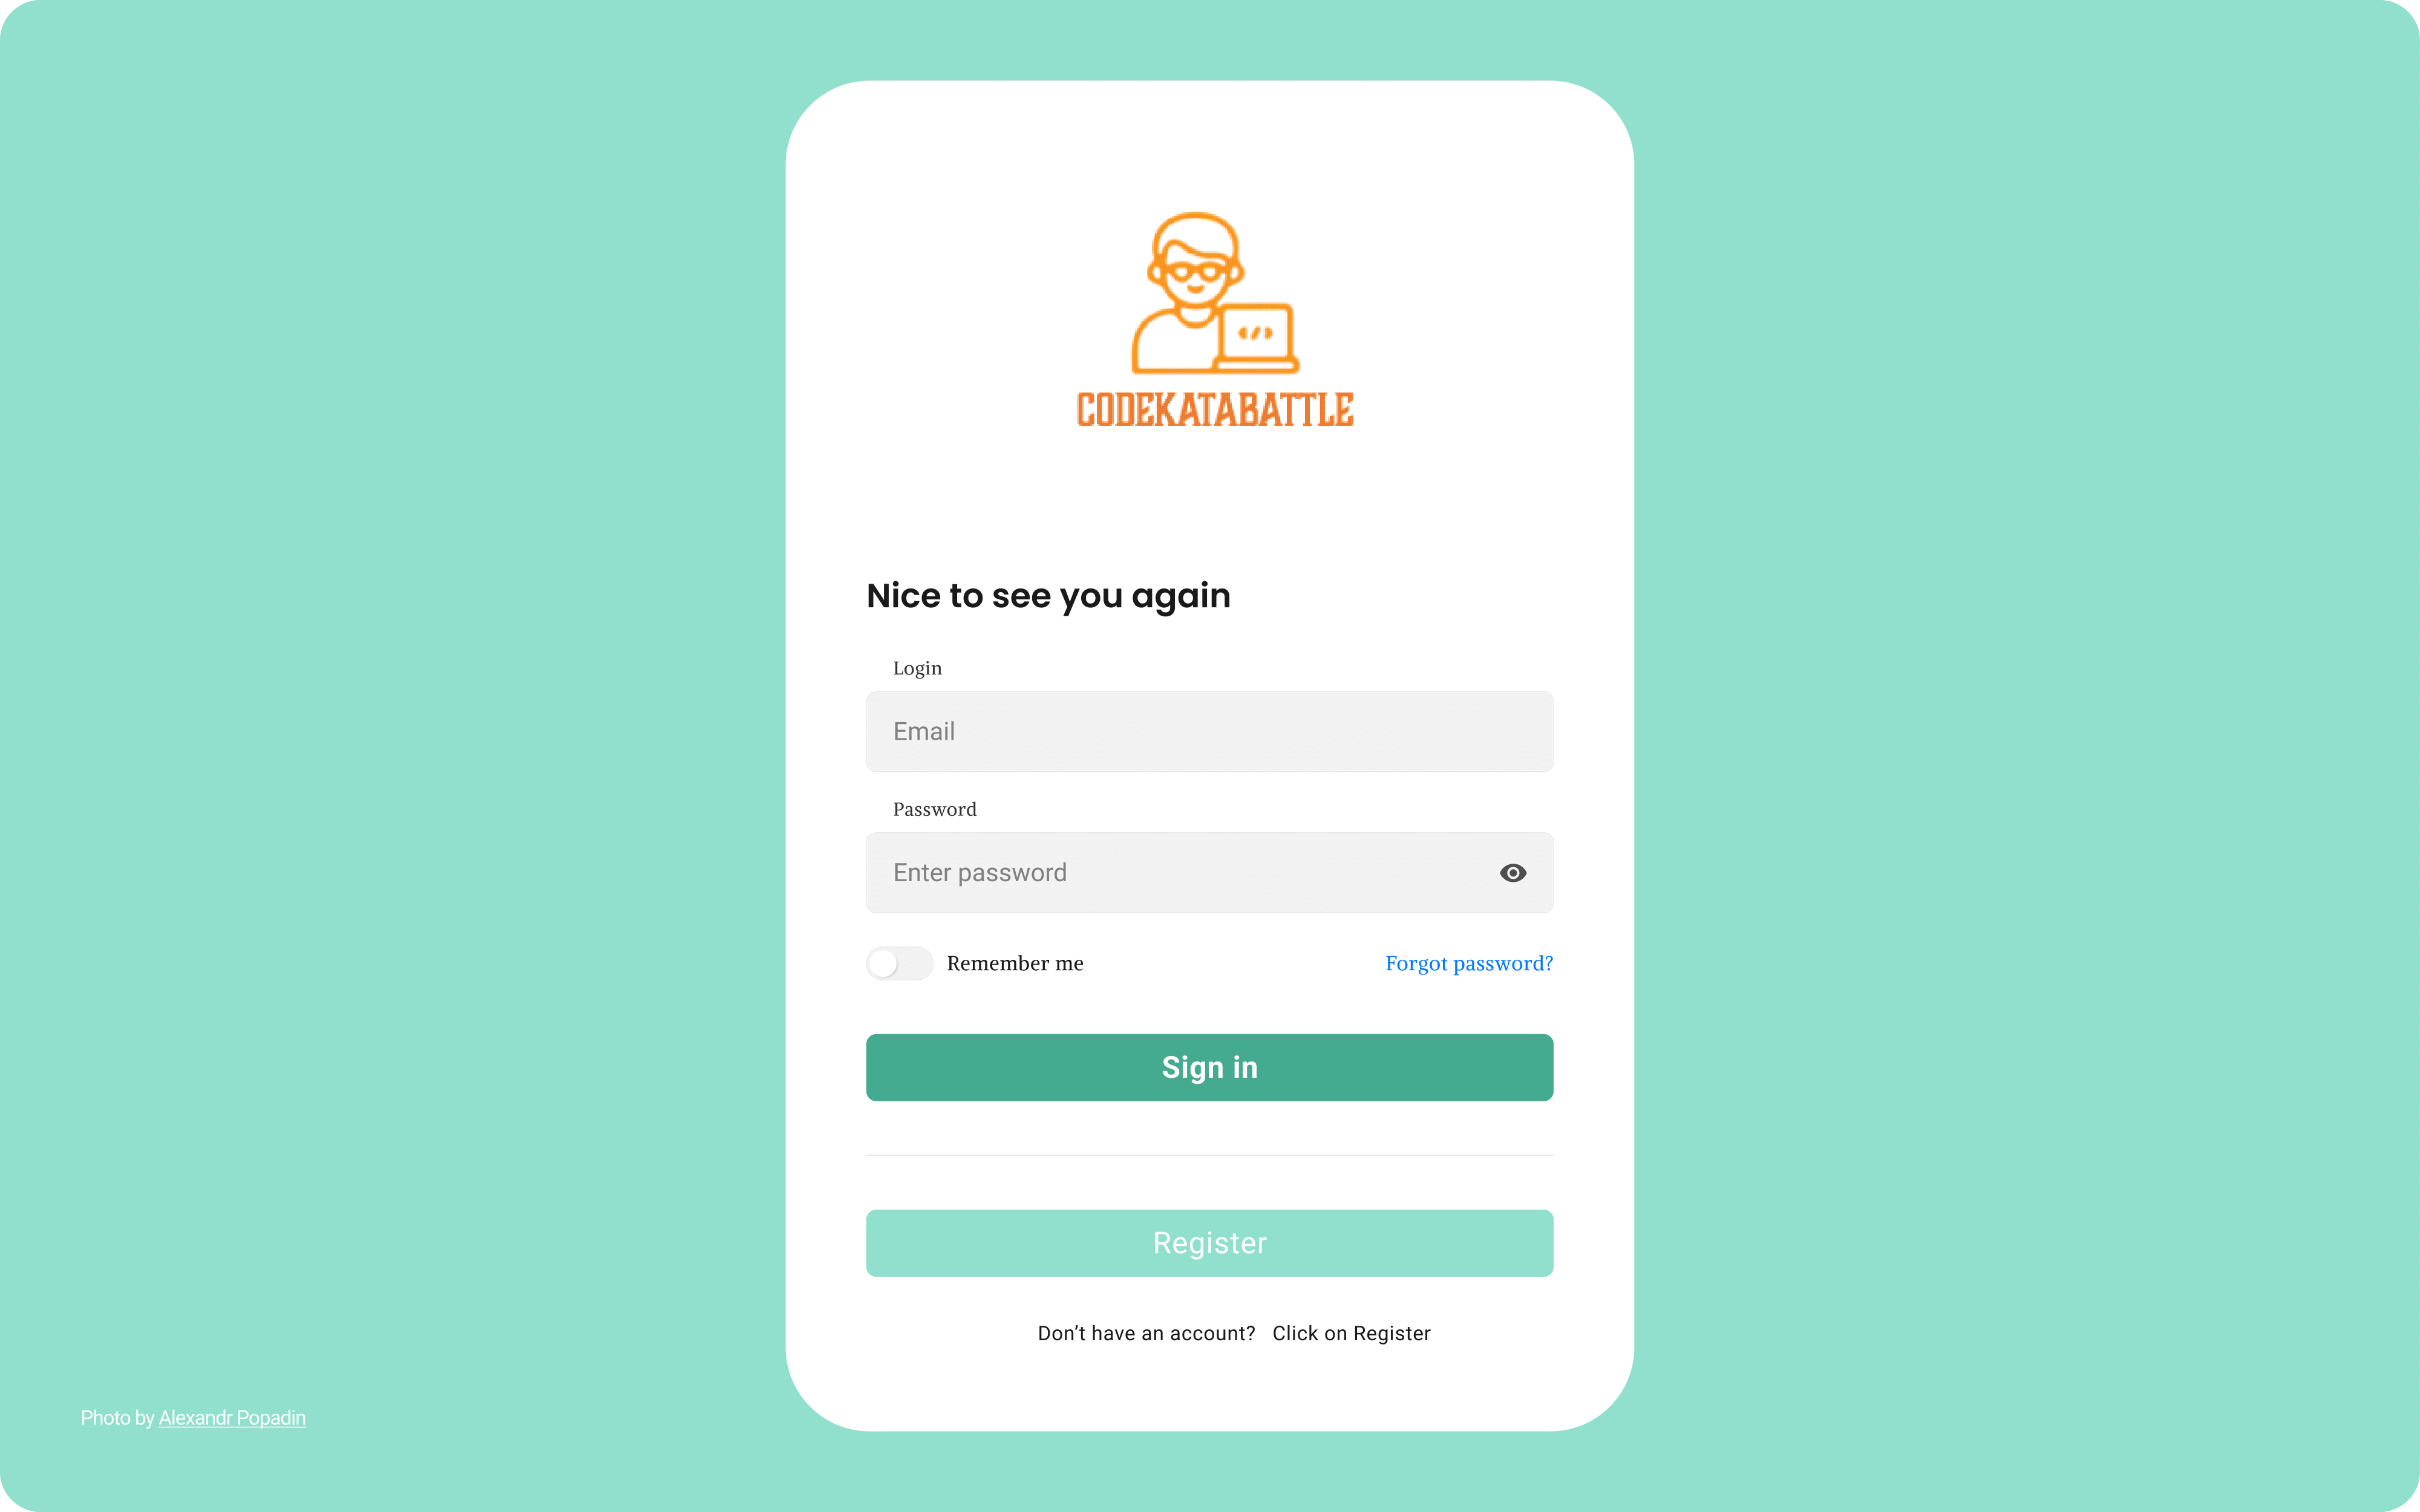
\includegraphics[width=0.8\textwidth]{images/user_interface/UI_sw2-01.png}
    \caption{Login page - same for all types of users}
\end{figure}

\begin{figure}[H]
    \centering
    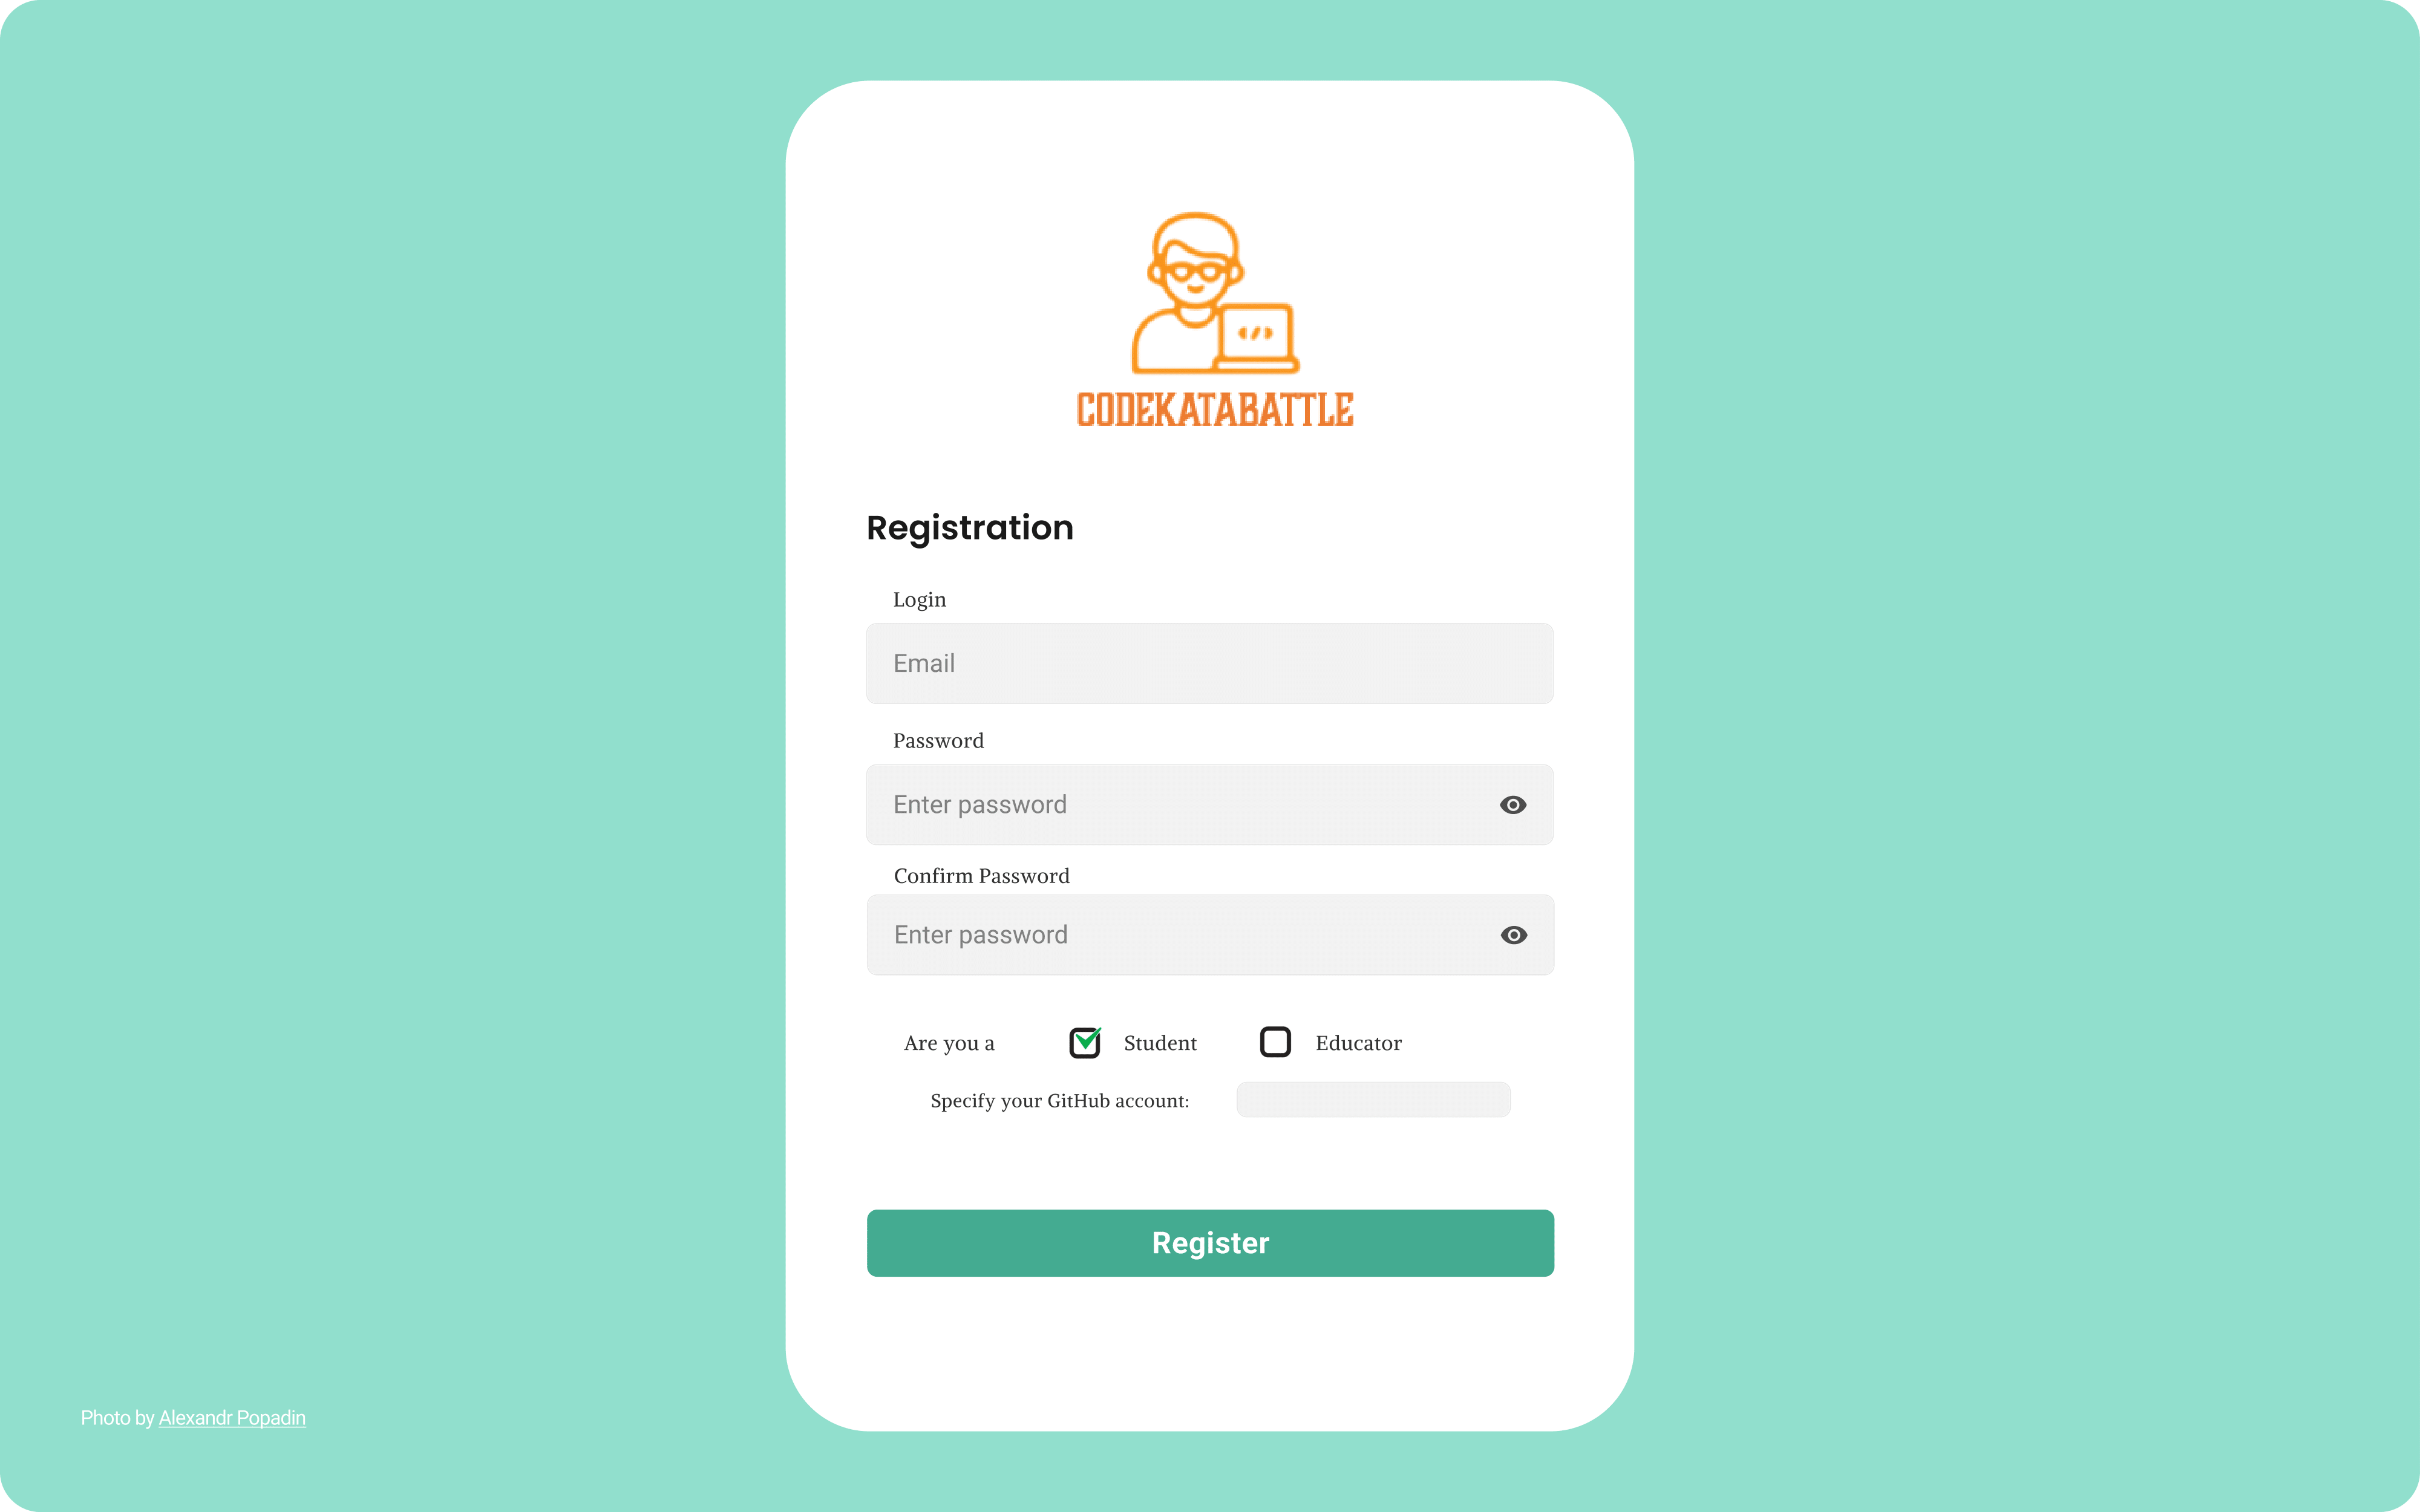
\includegraphics[width=0.8\textwidth]{images/user_interface/UI_sw2-02.png}
    \caption{Registration page - same for all types of users}
\end{figure}

\begin{figure}[H]
    \centering
    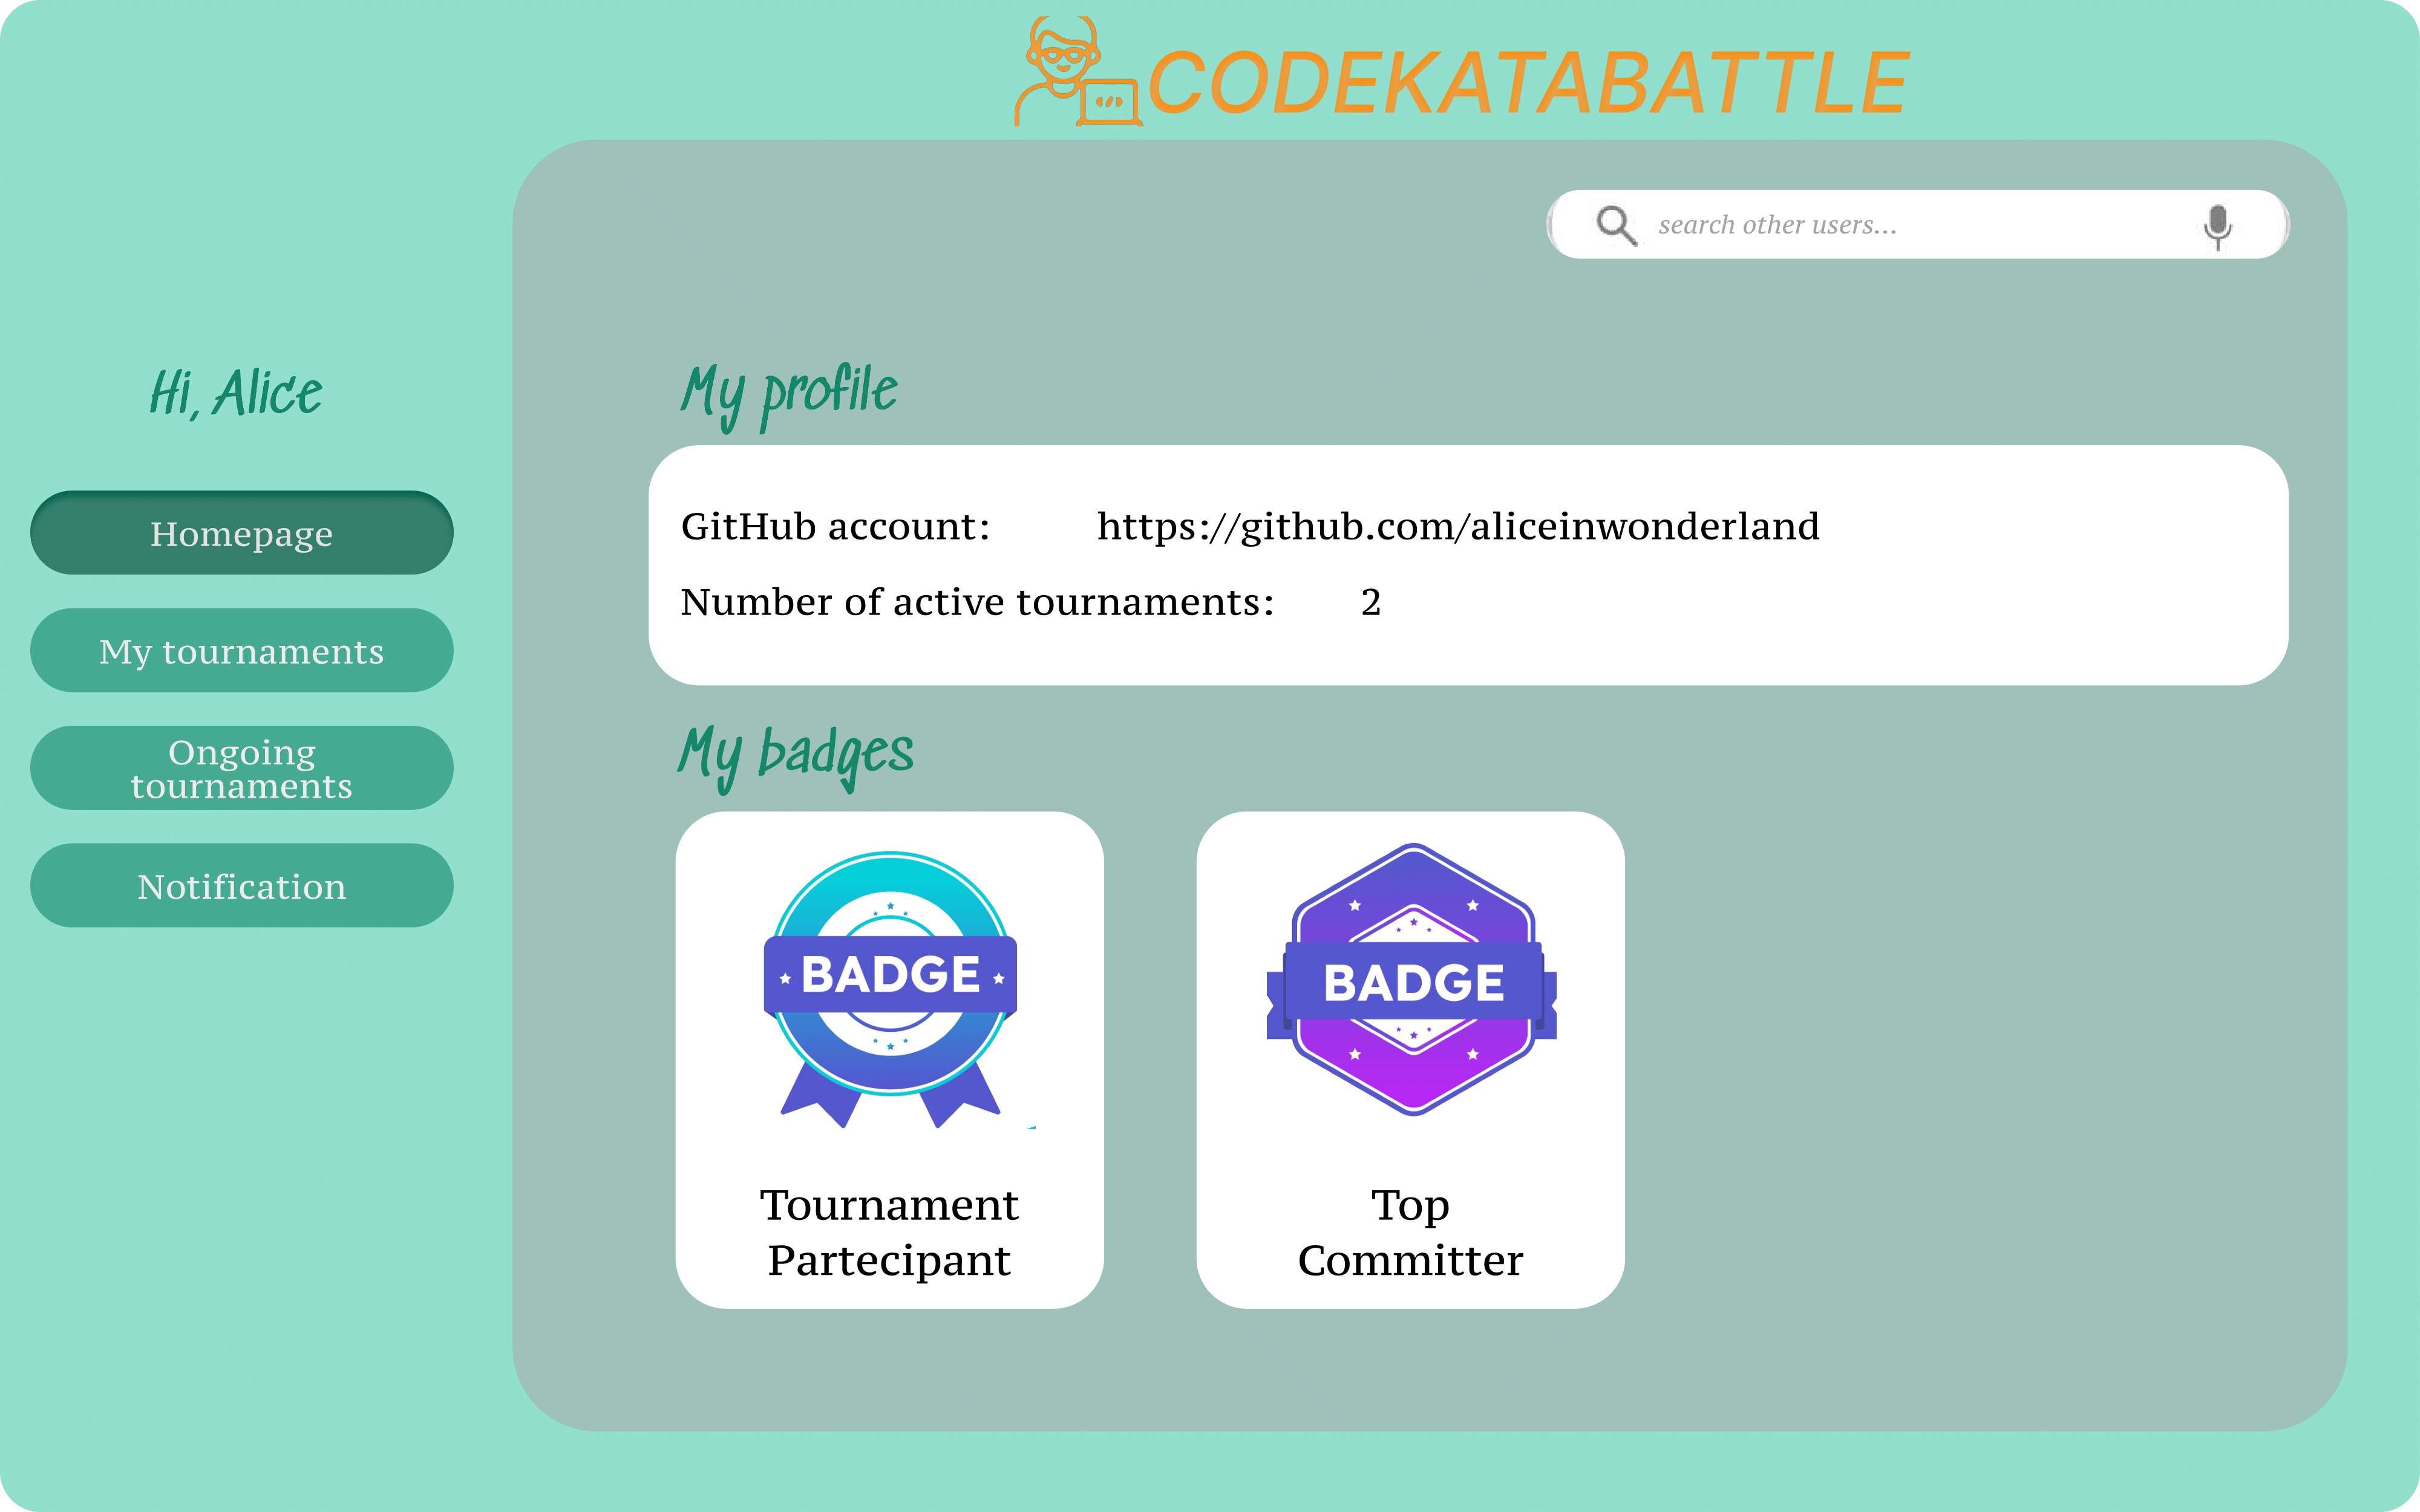
\includegraphics[width=0.8\textwidth]{images/user_interface/UI_sw2-03.png}
    \caption{Student's homepage and profile}
\end{figure}

\begin{figure}[H]
    \centering
    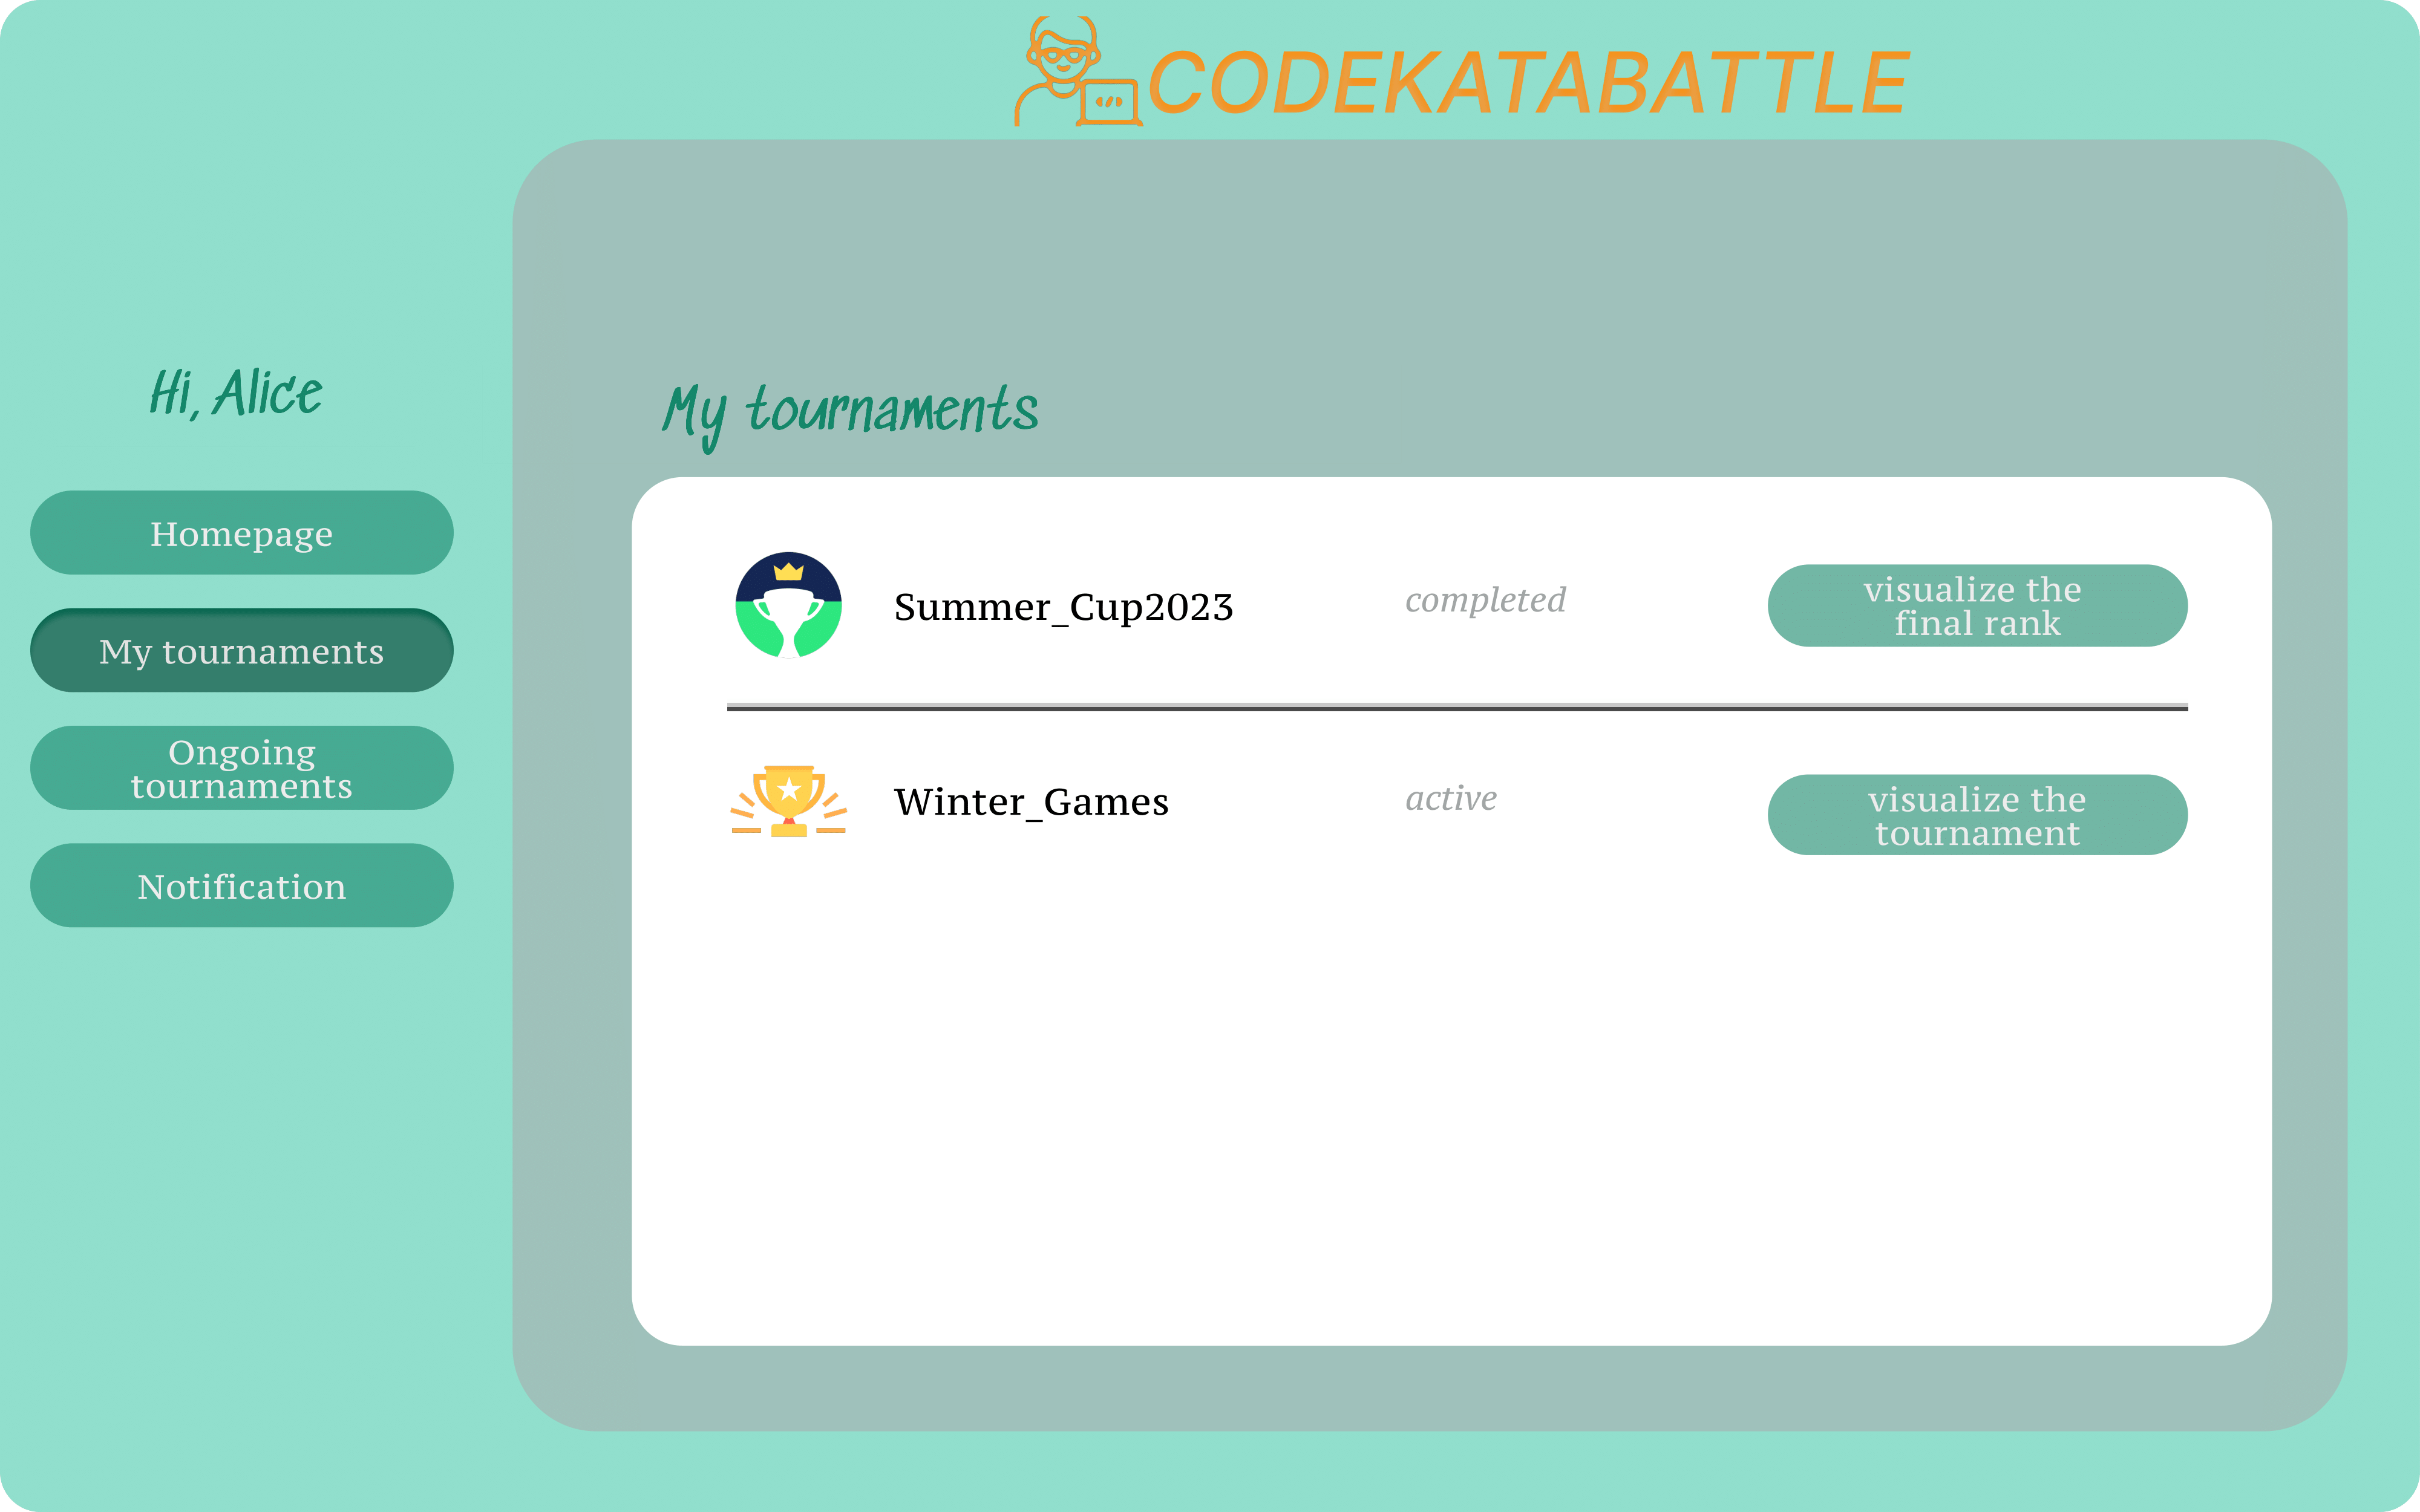
\includegraphics[width=0.8\textwidth]{images/user_interface/UI_sw2-04.png}
    \caption{My tournaments - student's page}
\end{figure}

\begin{figure}[H]
    \centering
    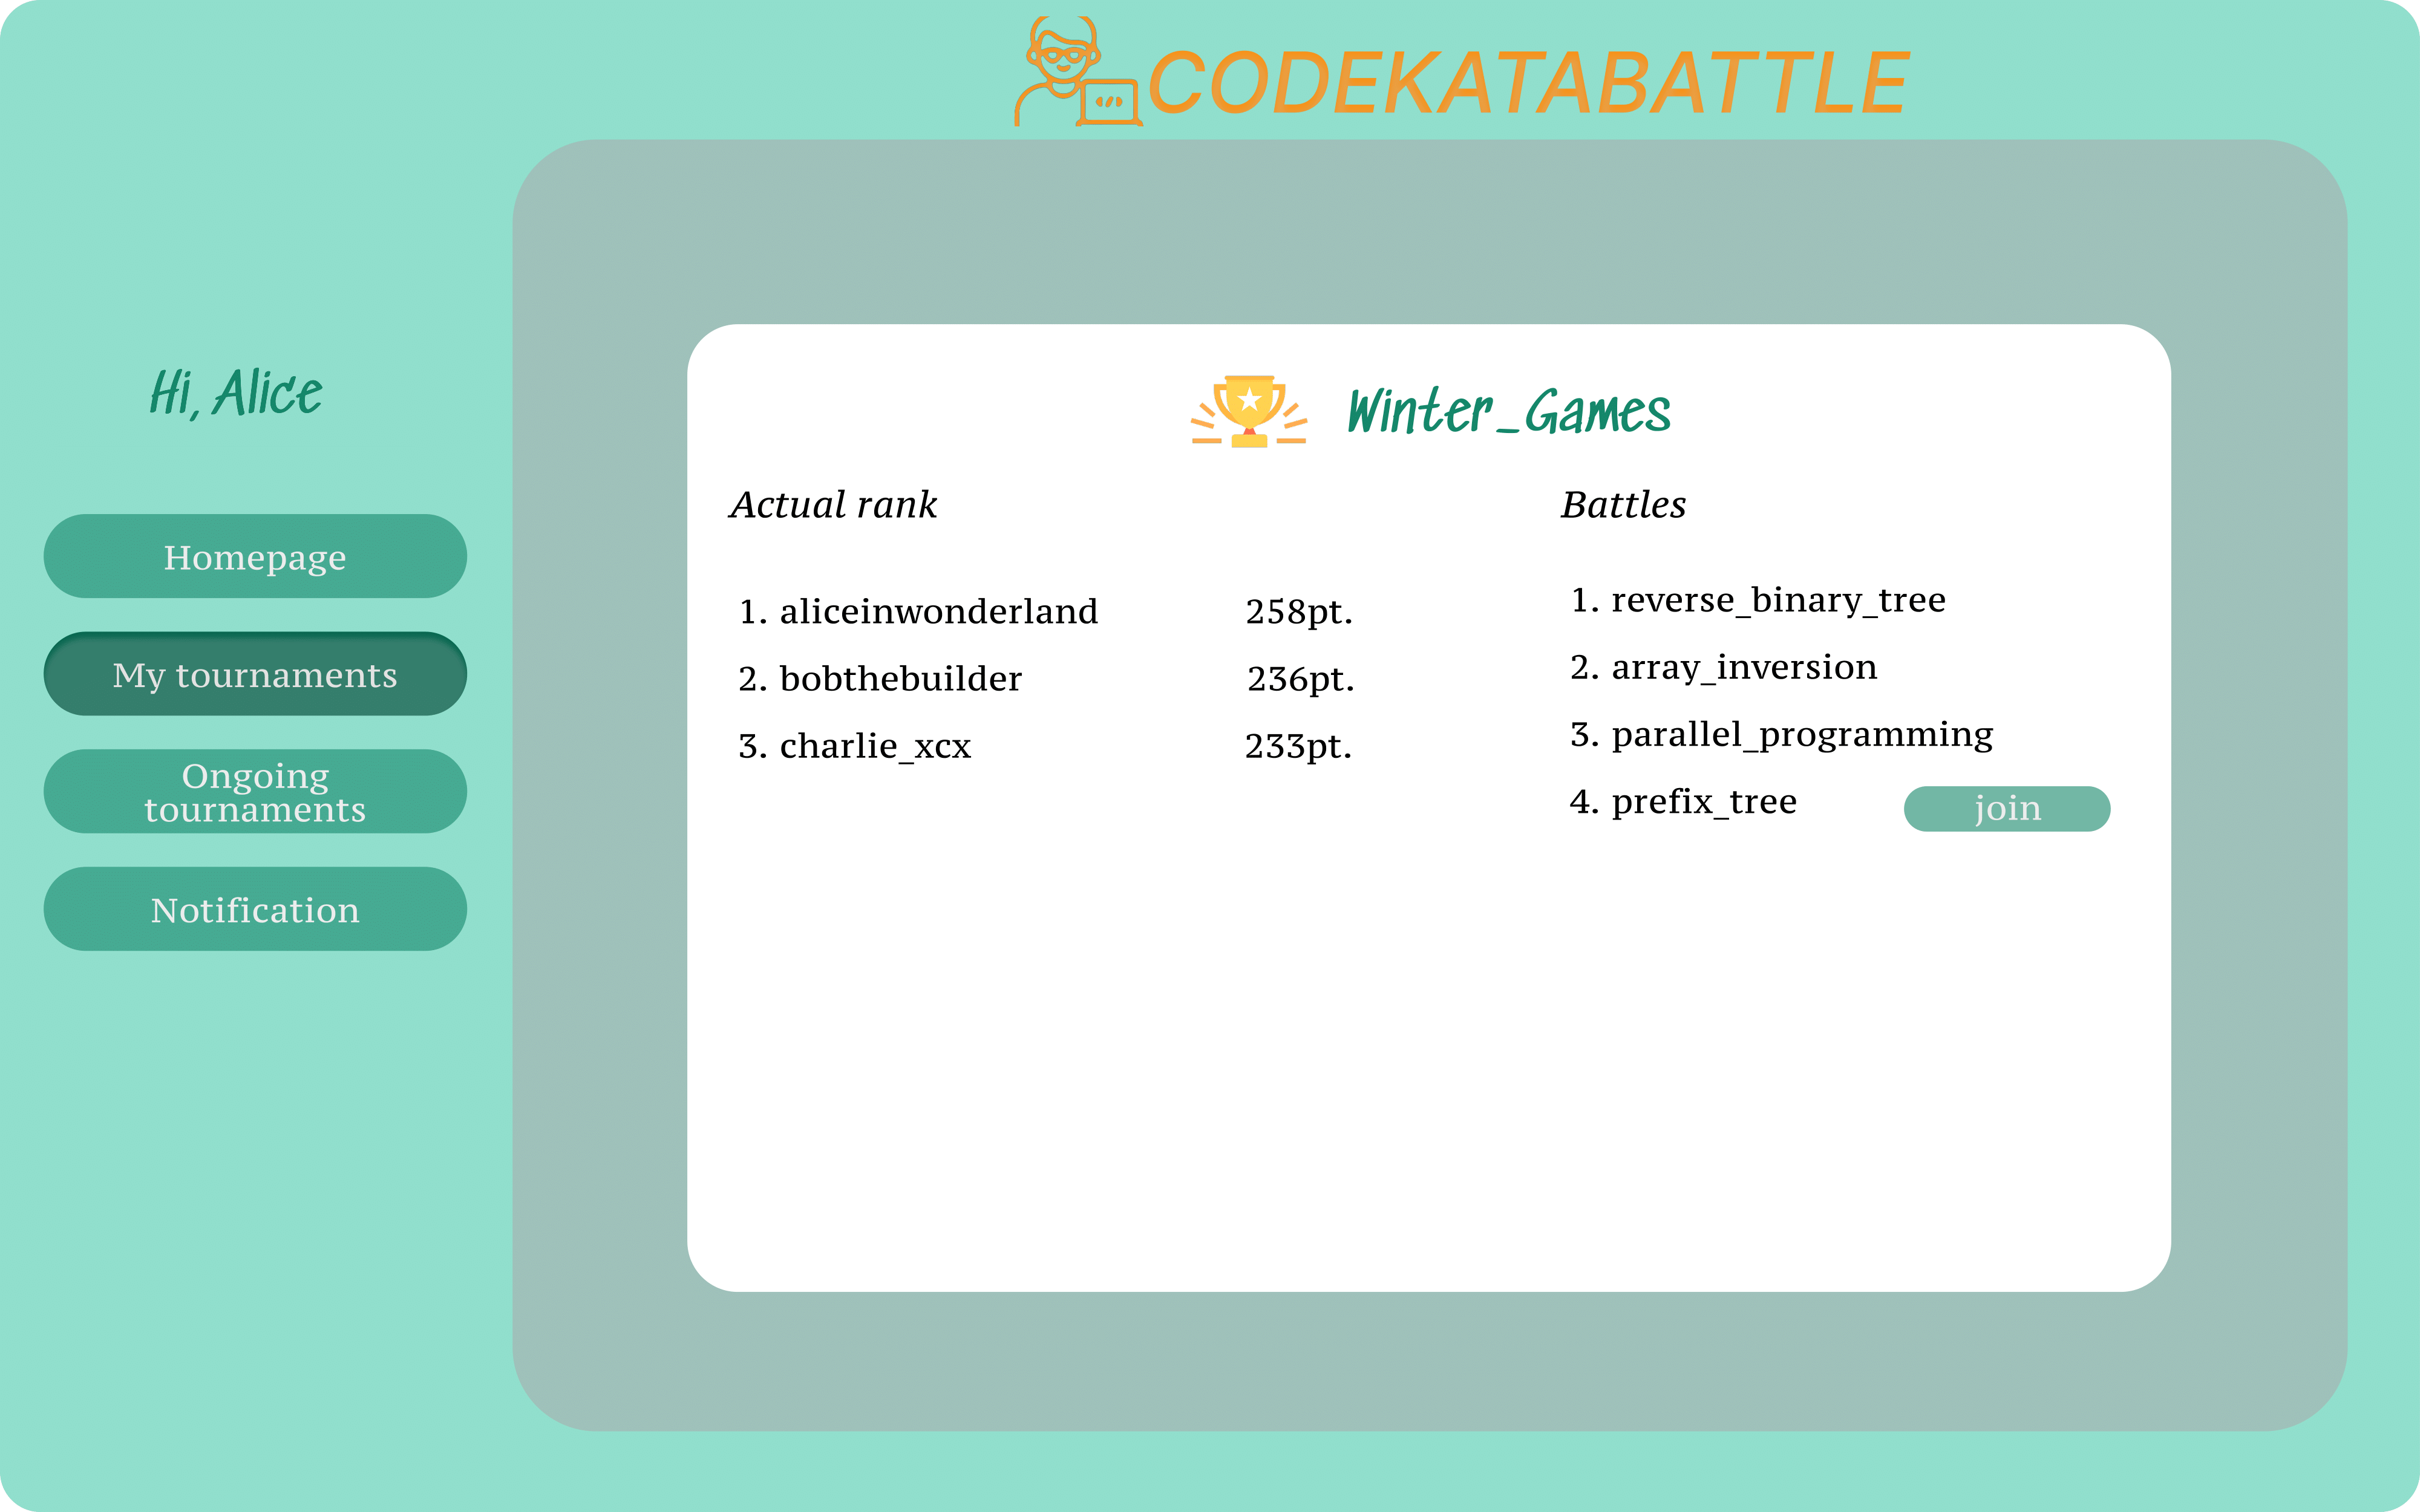
\includegraphics[width=0.8\textwidth]{images/user_interface/UI_sw2-05.png}
    \caption{Tournament's details - student's page}
\end{figure}

\begin{figure}[H]
    \centering
    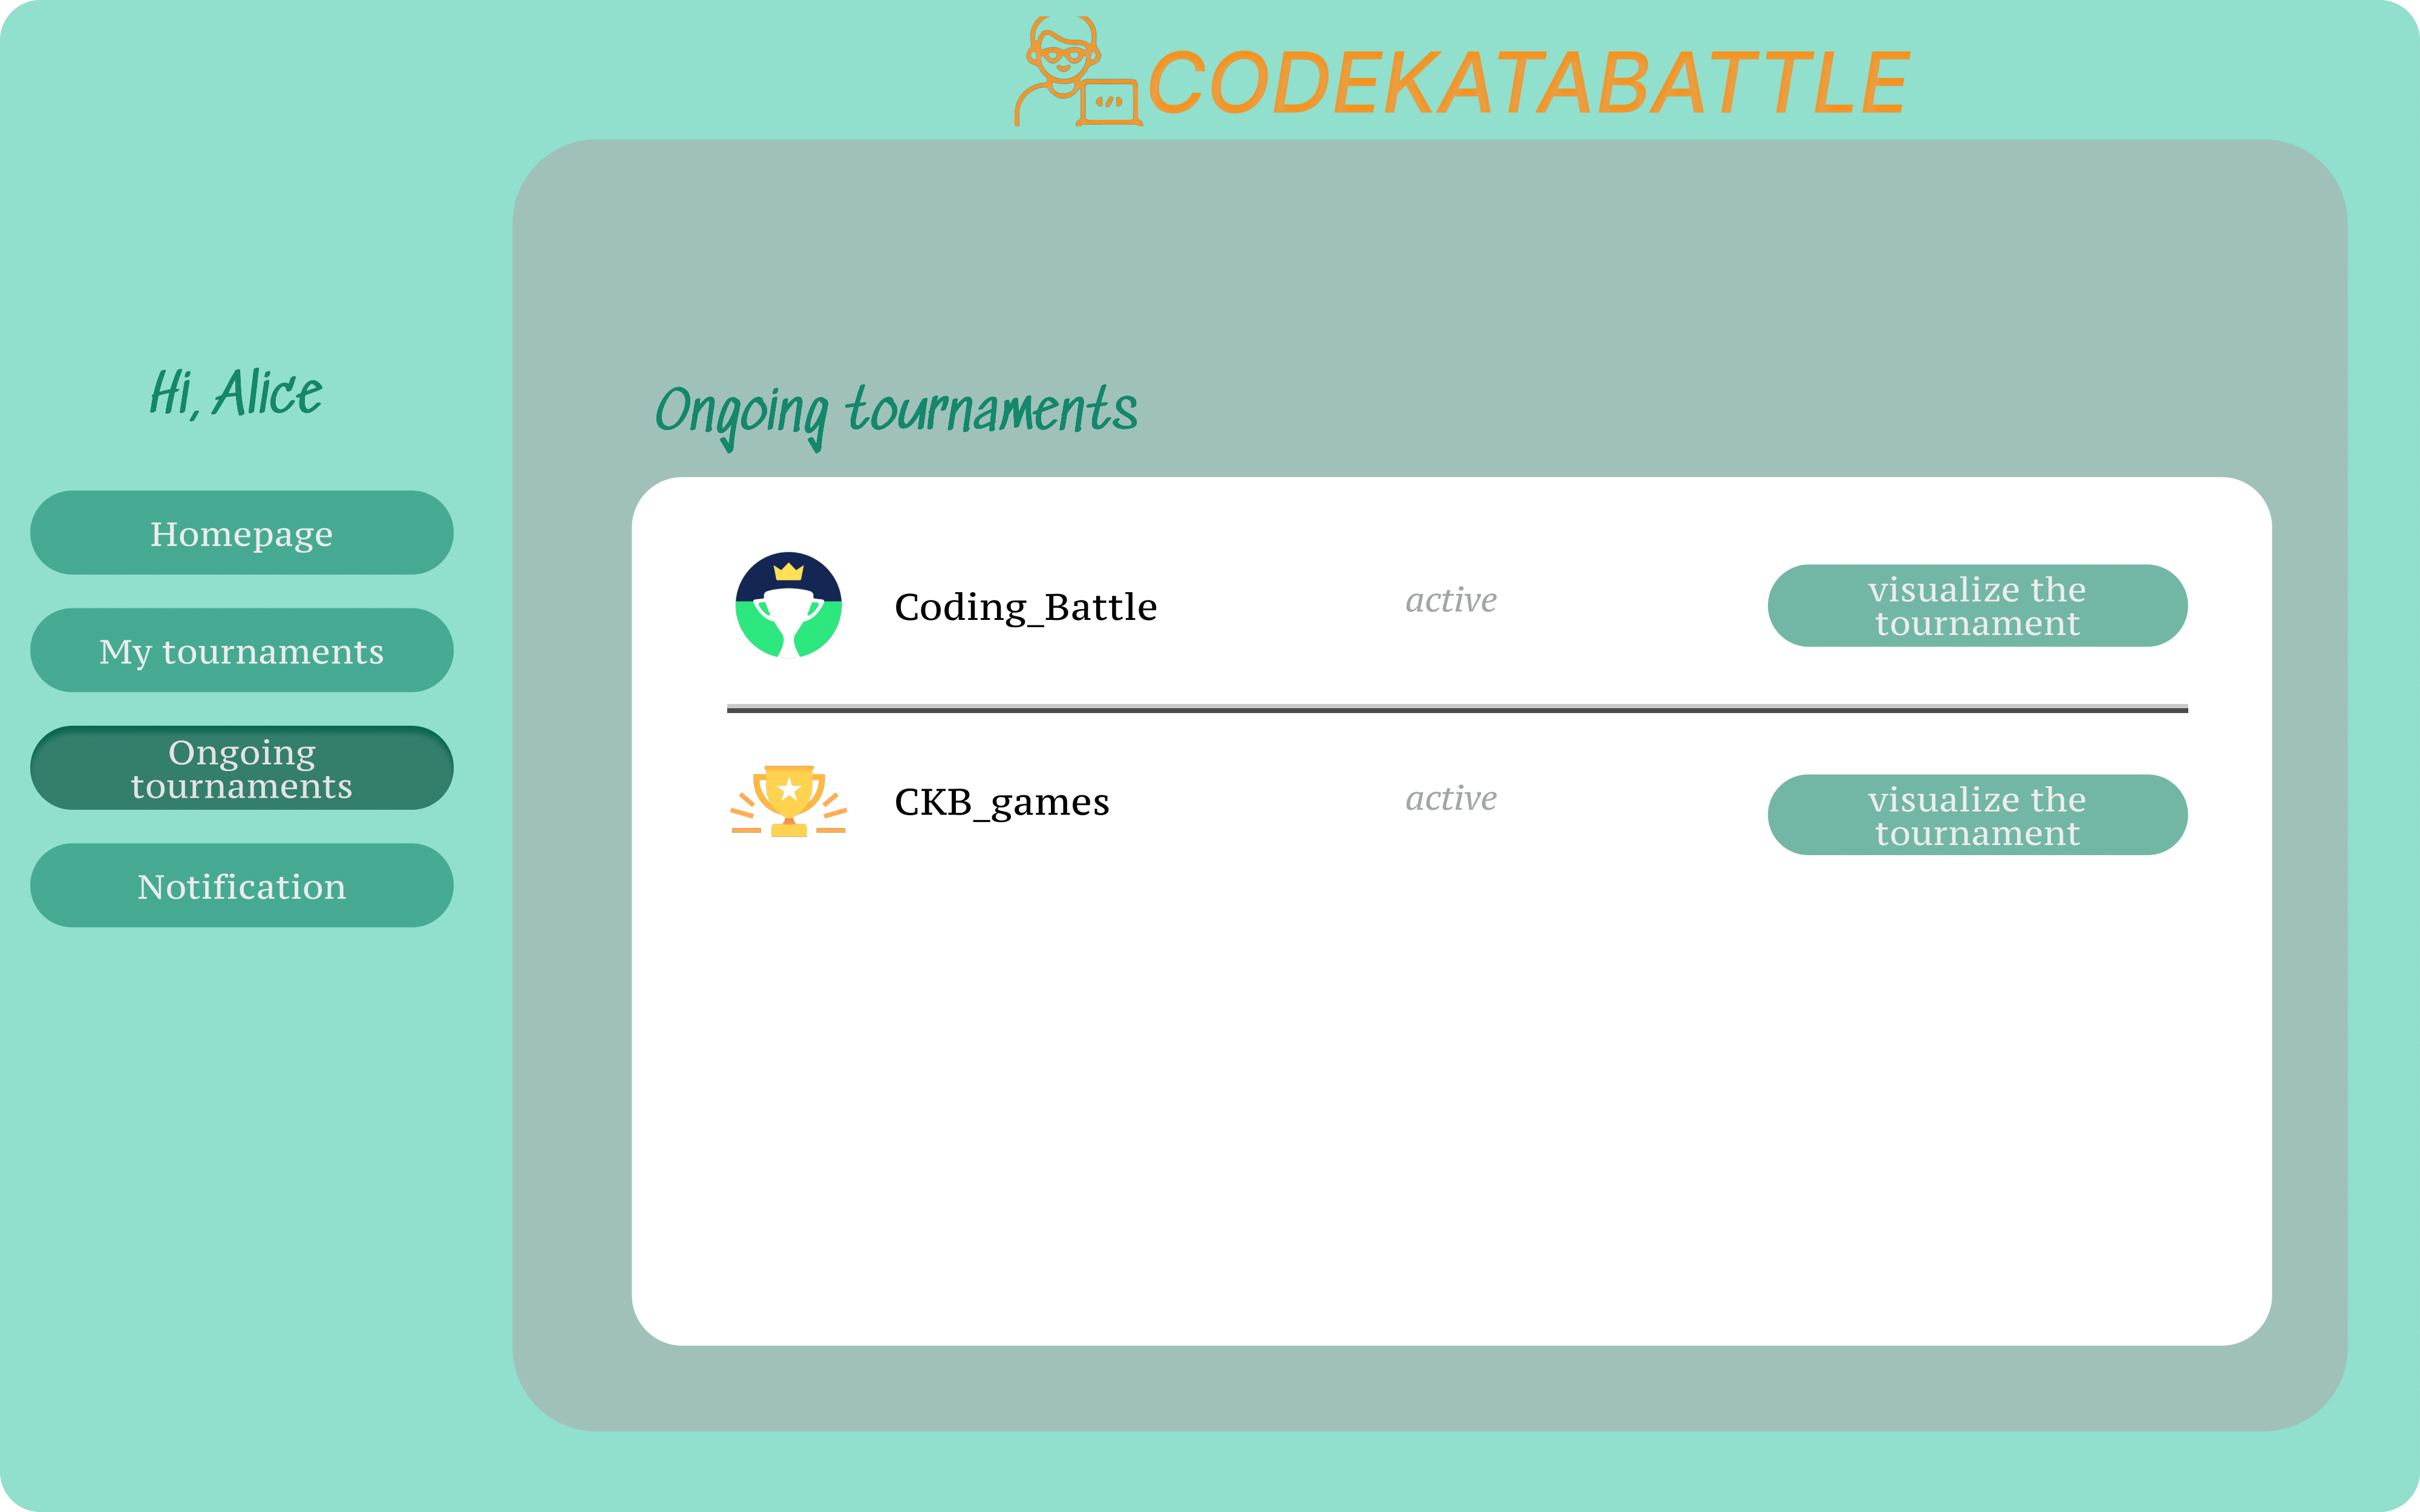
\includegraphics[width=0.8\textwidth]{images/user_interface/UI_sw2-06.png}
    \caption{Ongoing tournaments - student's page}
\end{figure}

\begin{figure}[H]
    \centering
    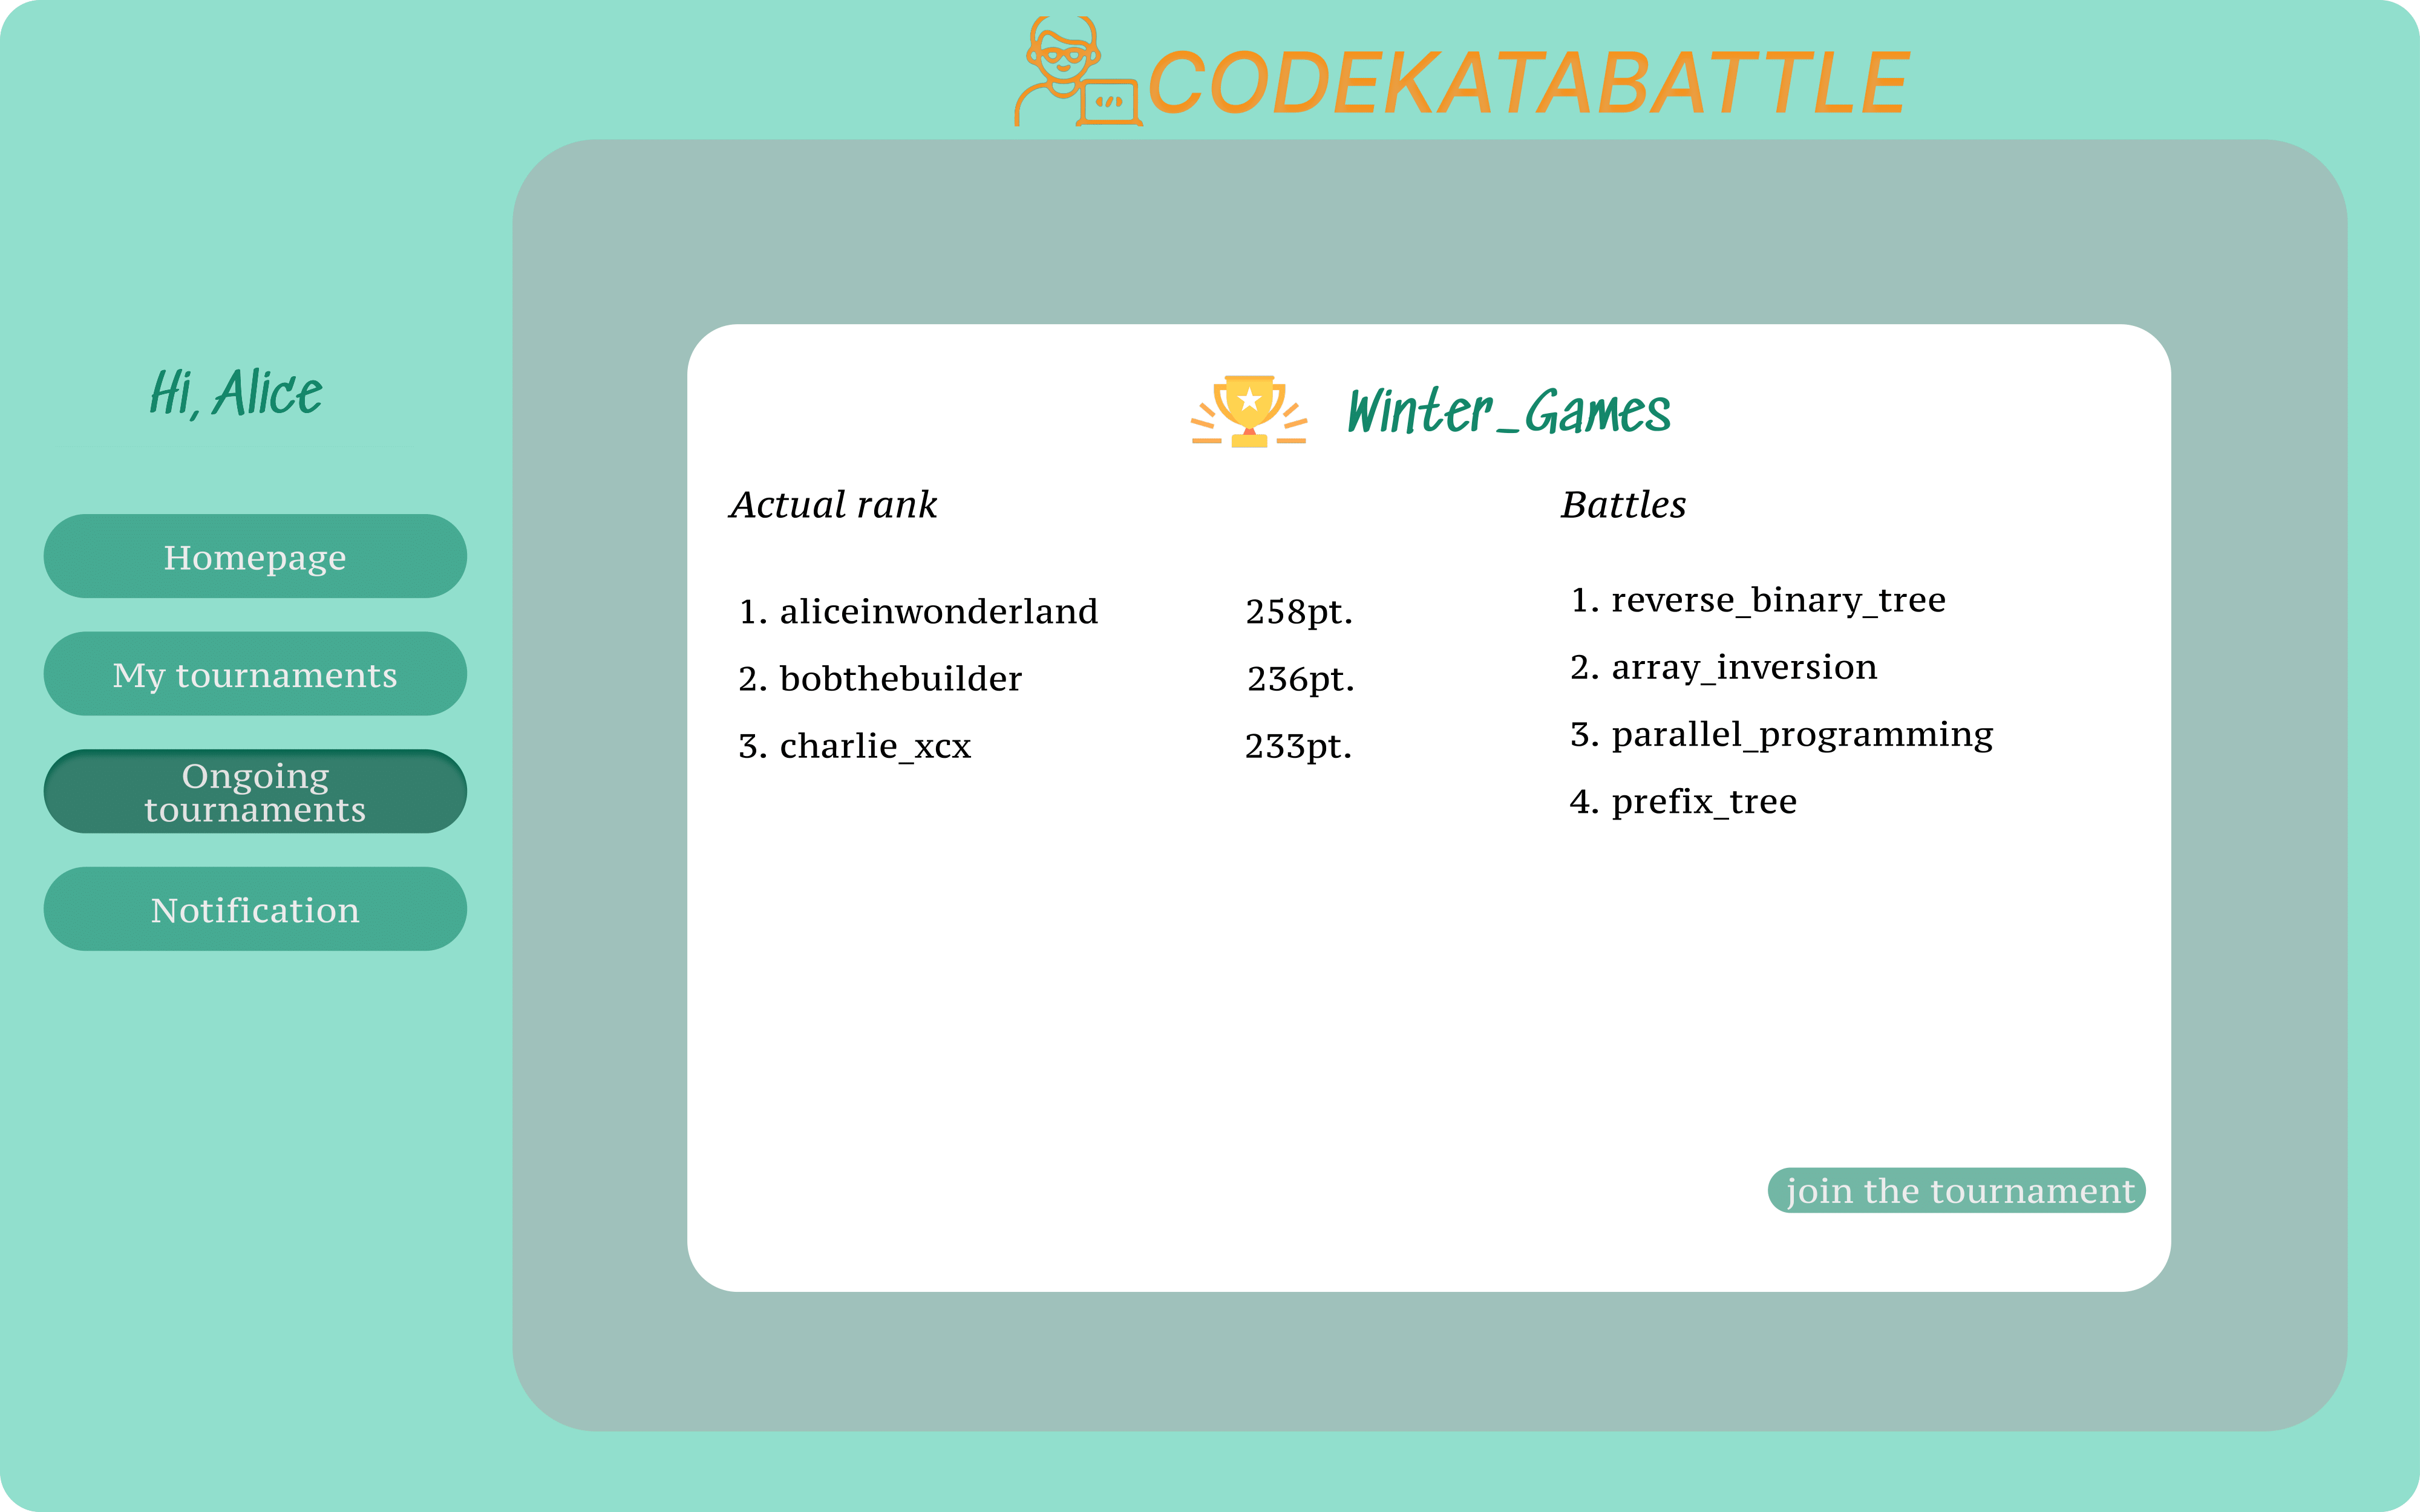
\includegraphics[width=0.8\textwidth]{images/user_interface/UI_sw2-07.png}
    \caption{Join a new tournament - student's page}
\end{figure}

\begin{figure}[H]
    \centering
    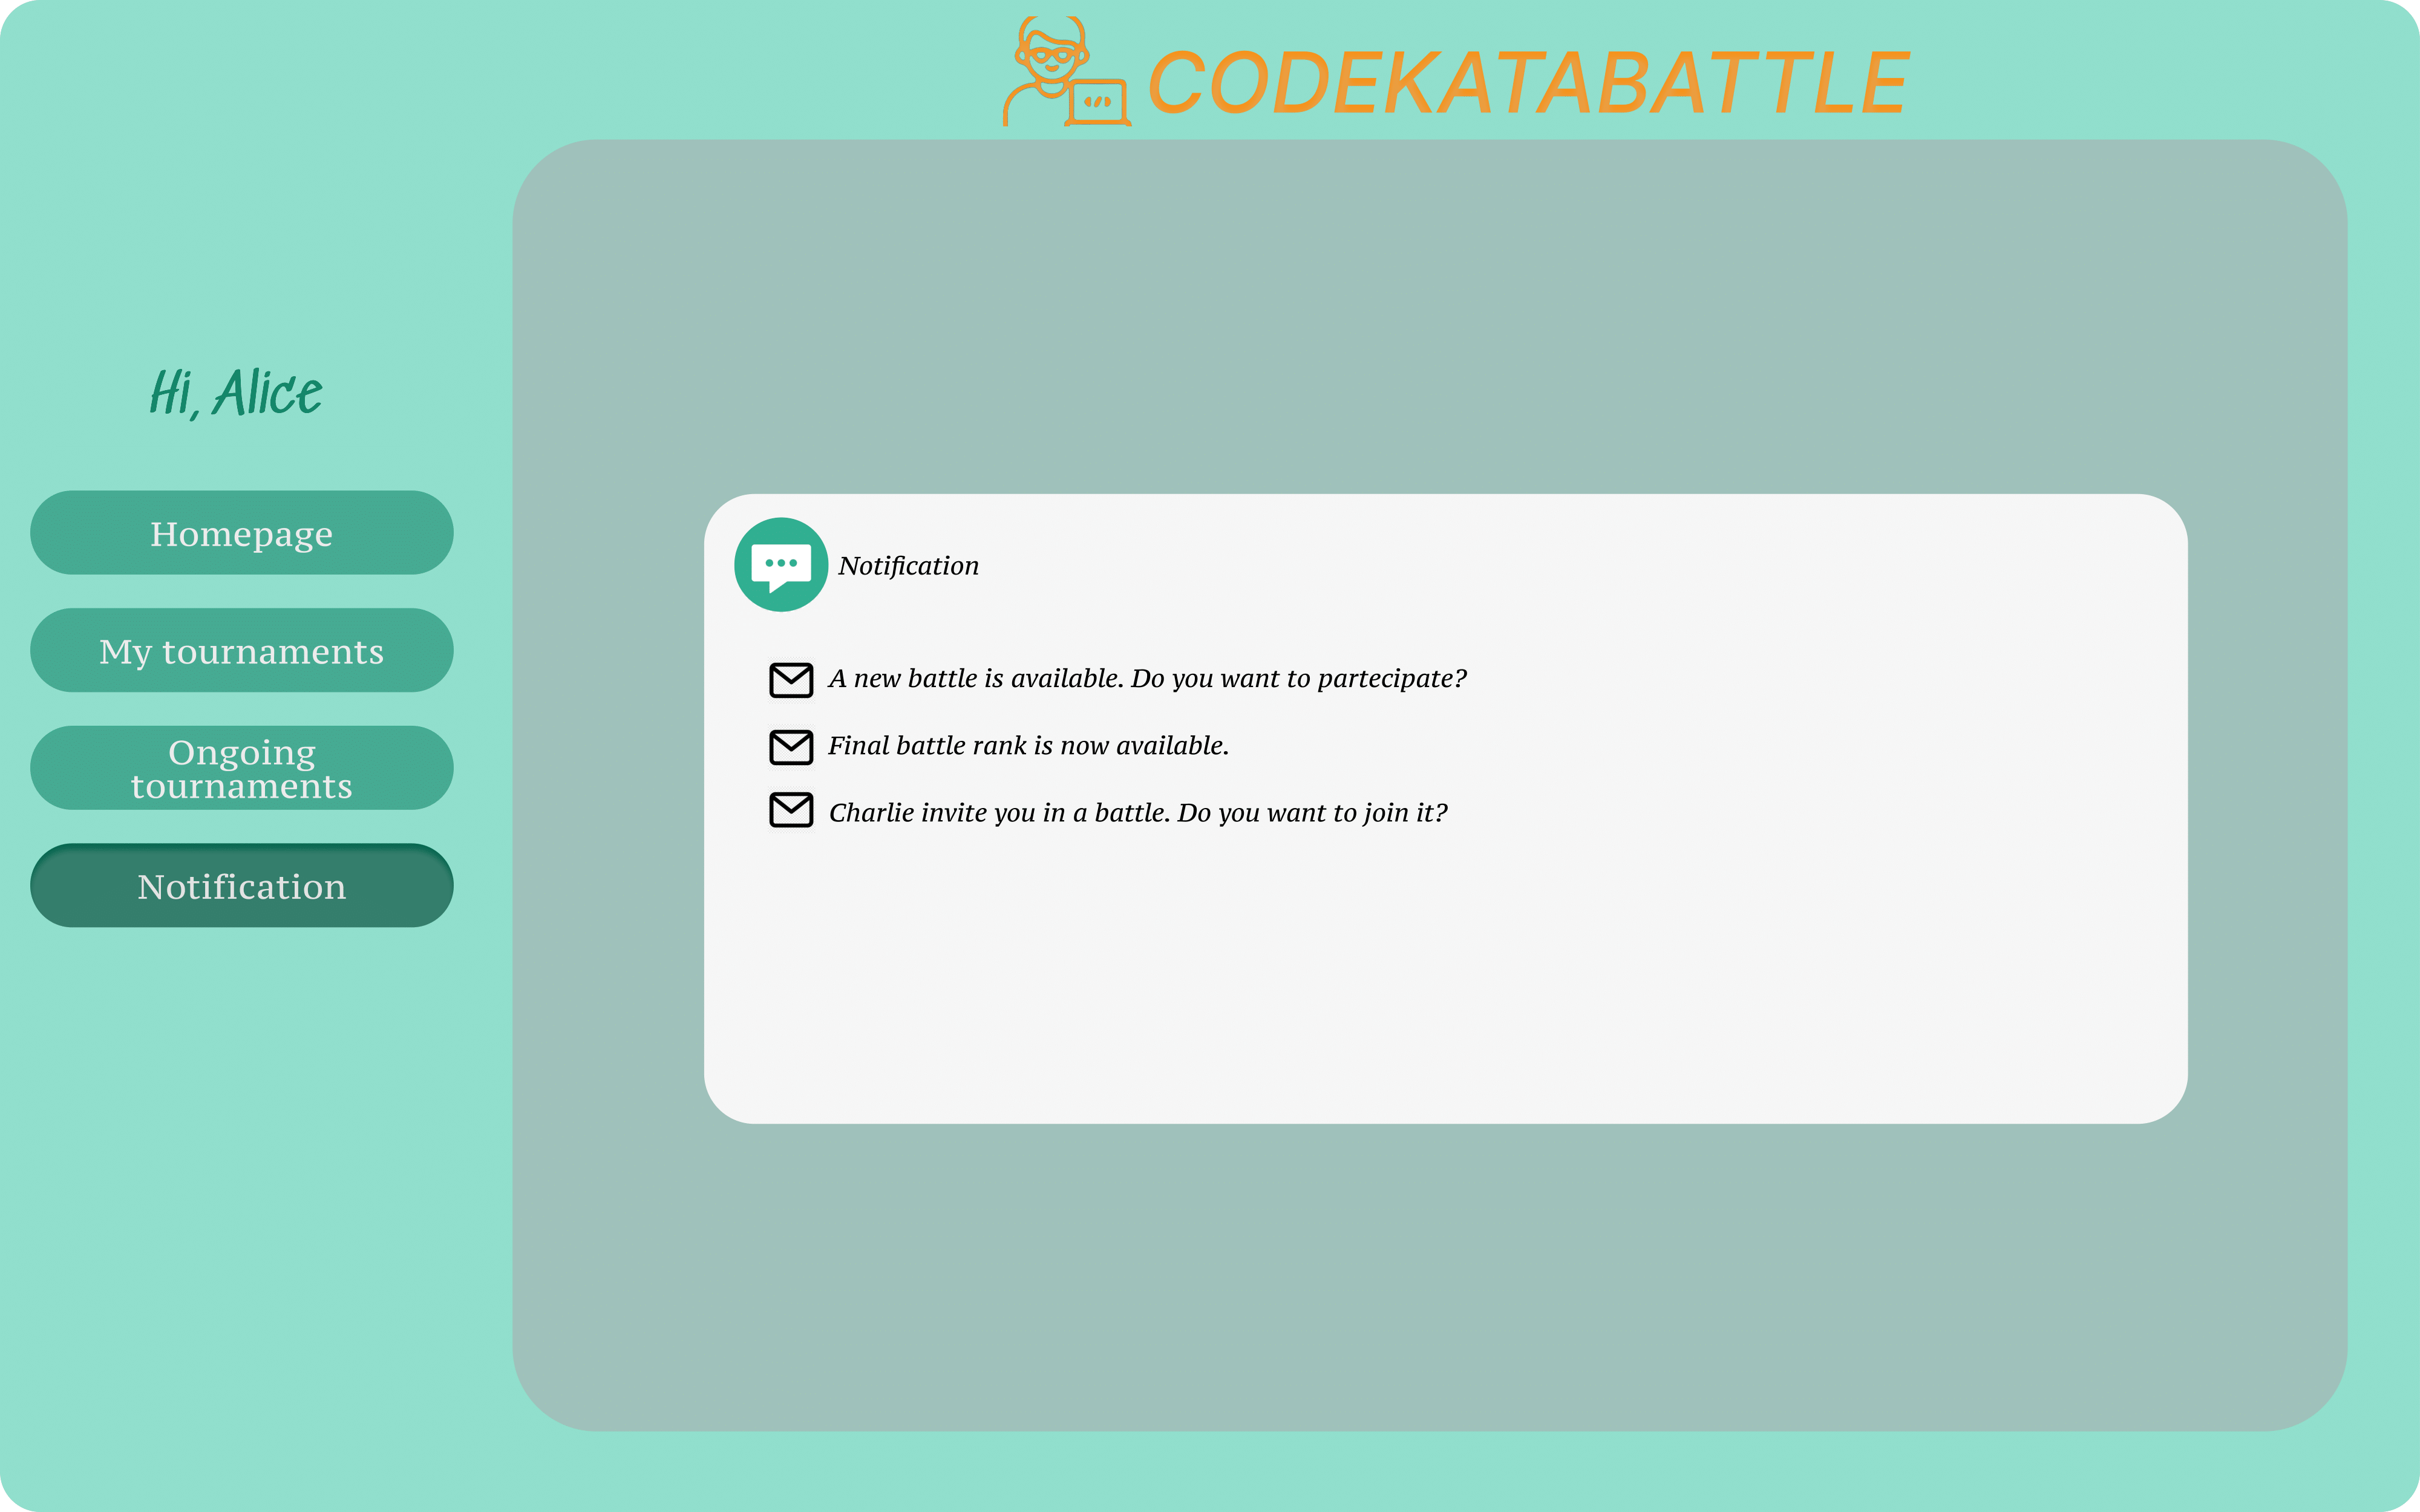
\includegraphics[width=0.8\textwidth]{images/user_interface/UI_sw2-08.png}
    \caption{Notification page - student's page}
\end{figure}

\begin{figure}[H]
    \centering
    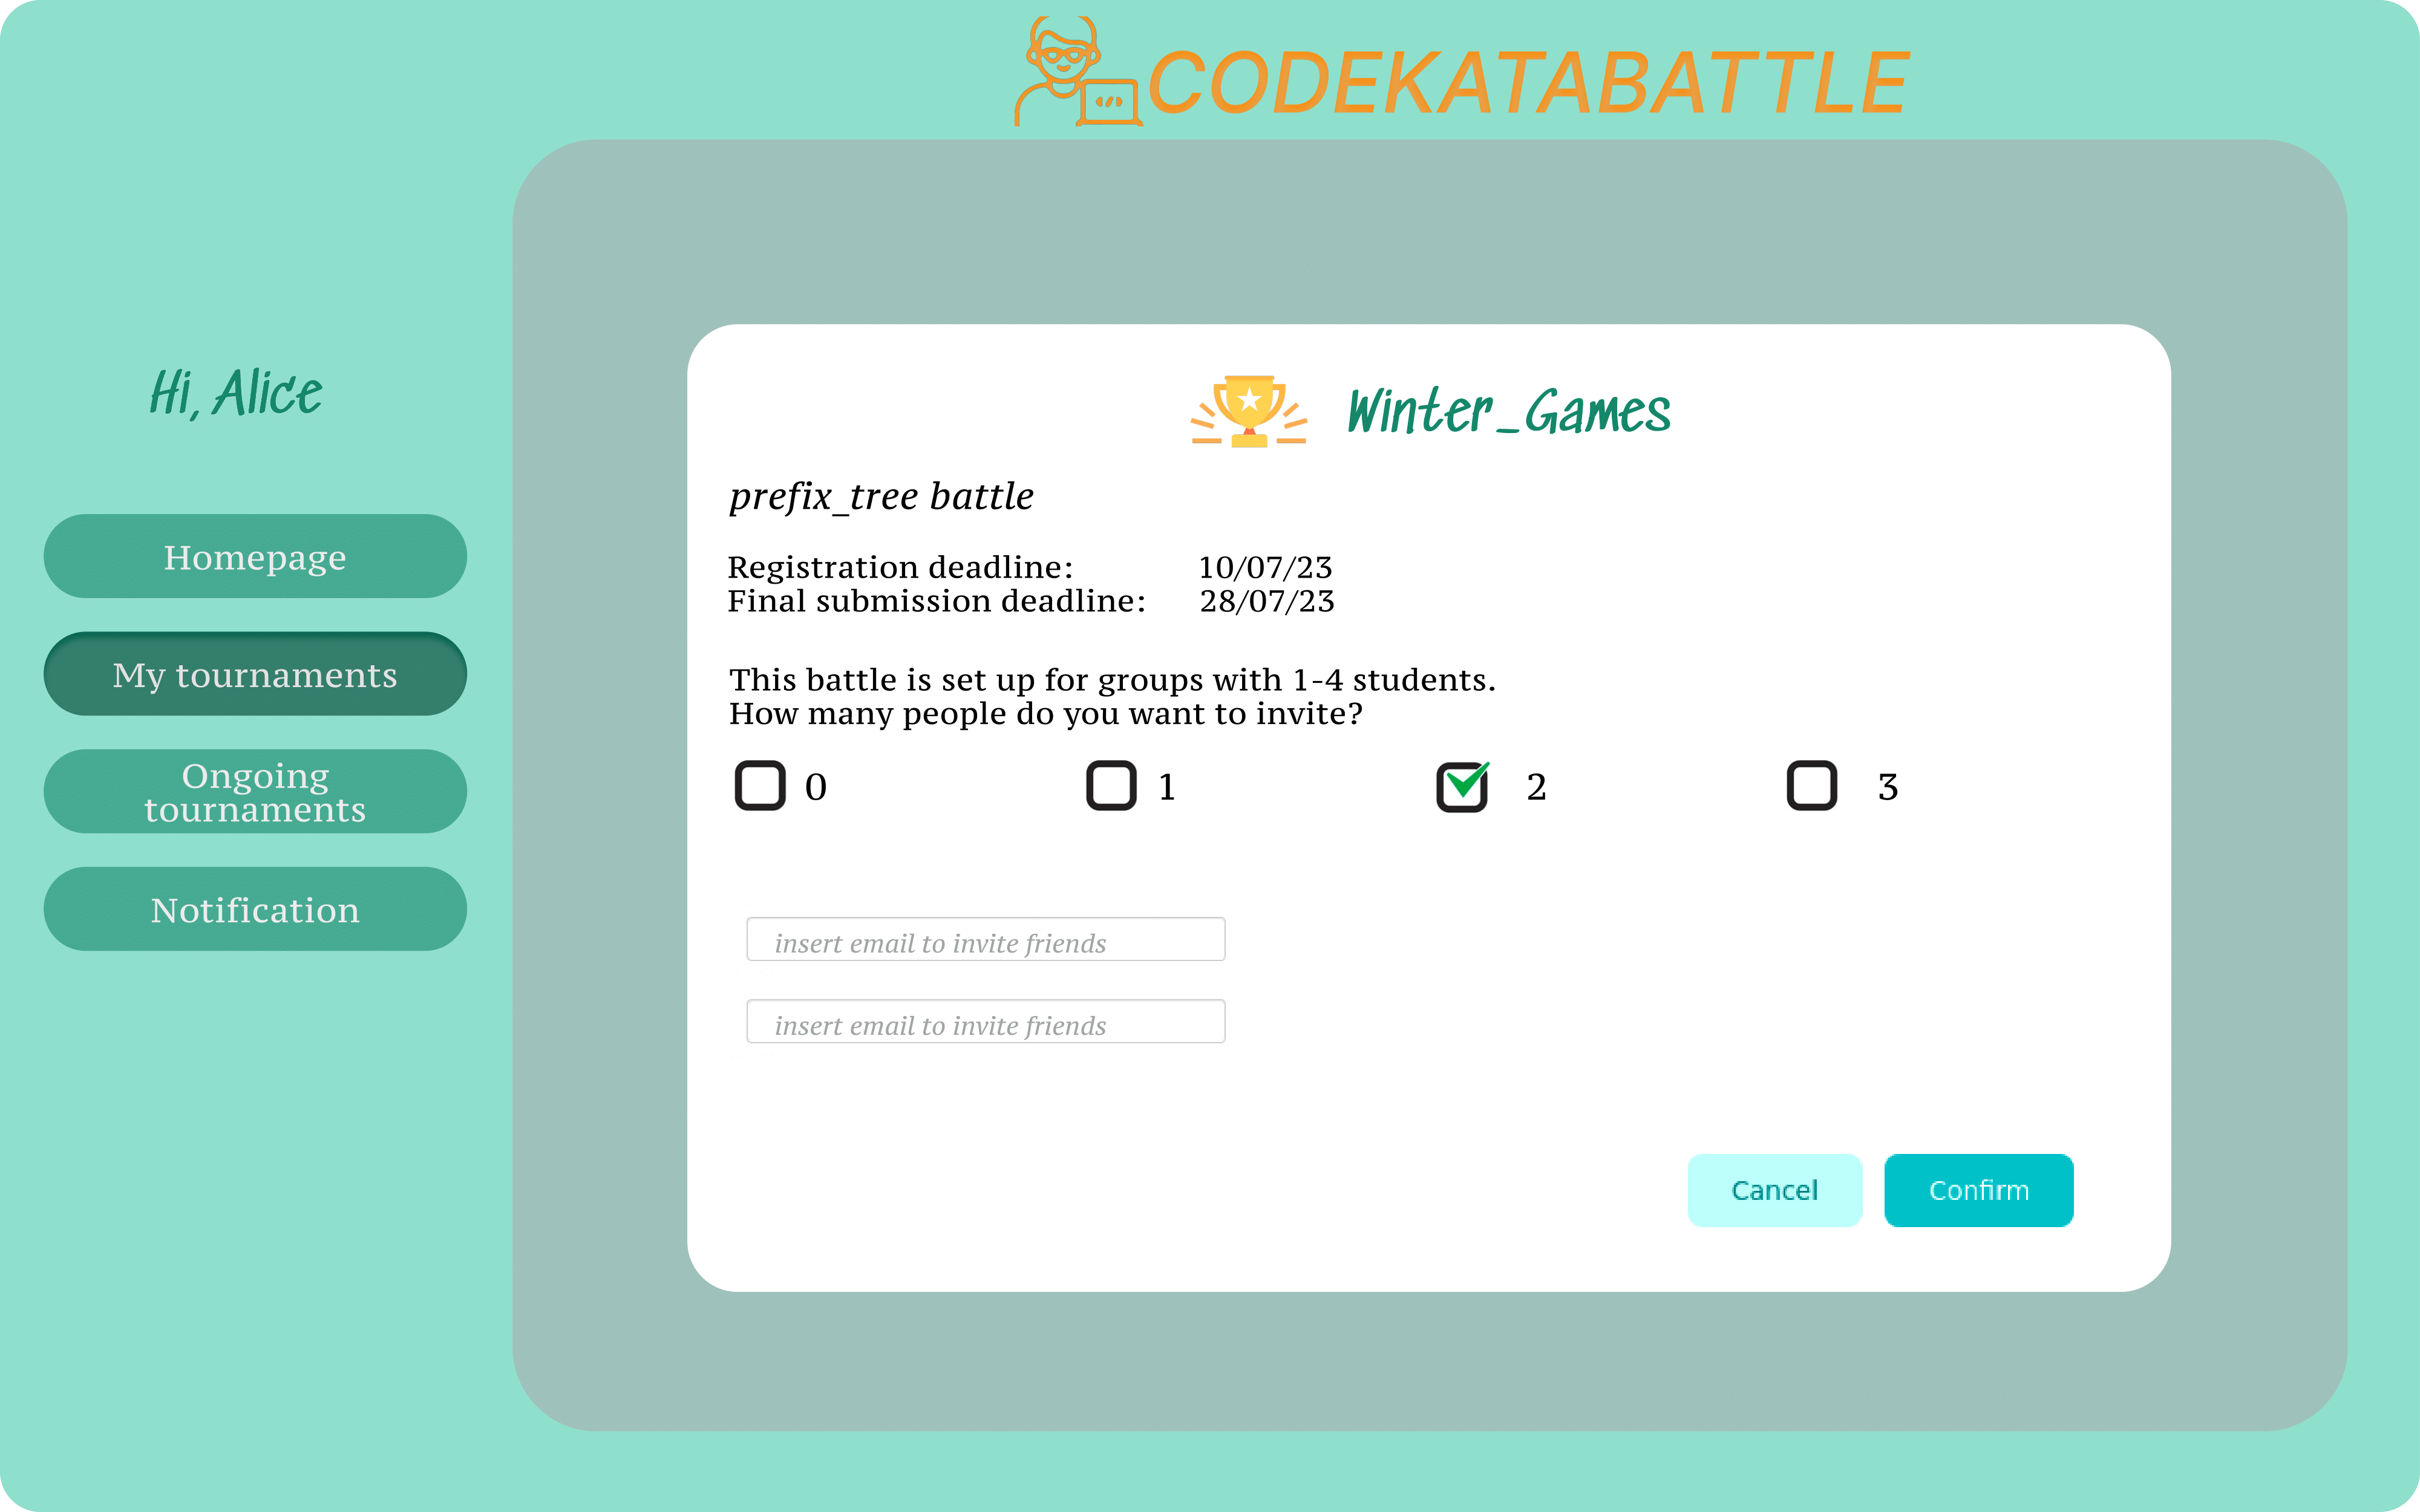
\includegraphics[width=0.8\textwidth]{images/user_interface/UI_sw2-09.png}
    \caption{Submission of a new battle - student's page}
\end{figure}

\begin{figure}[H]
    \centering
    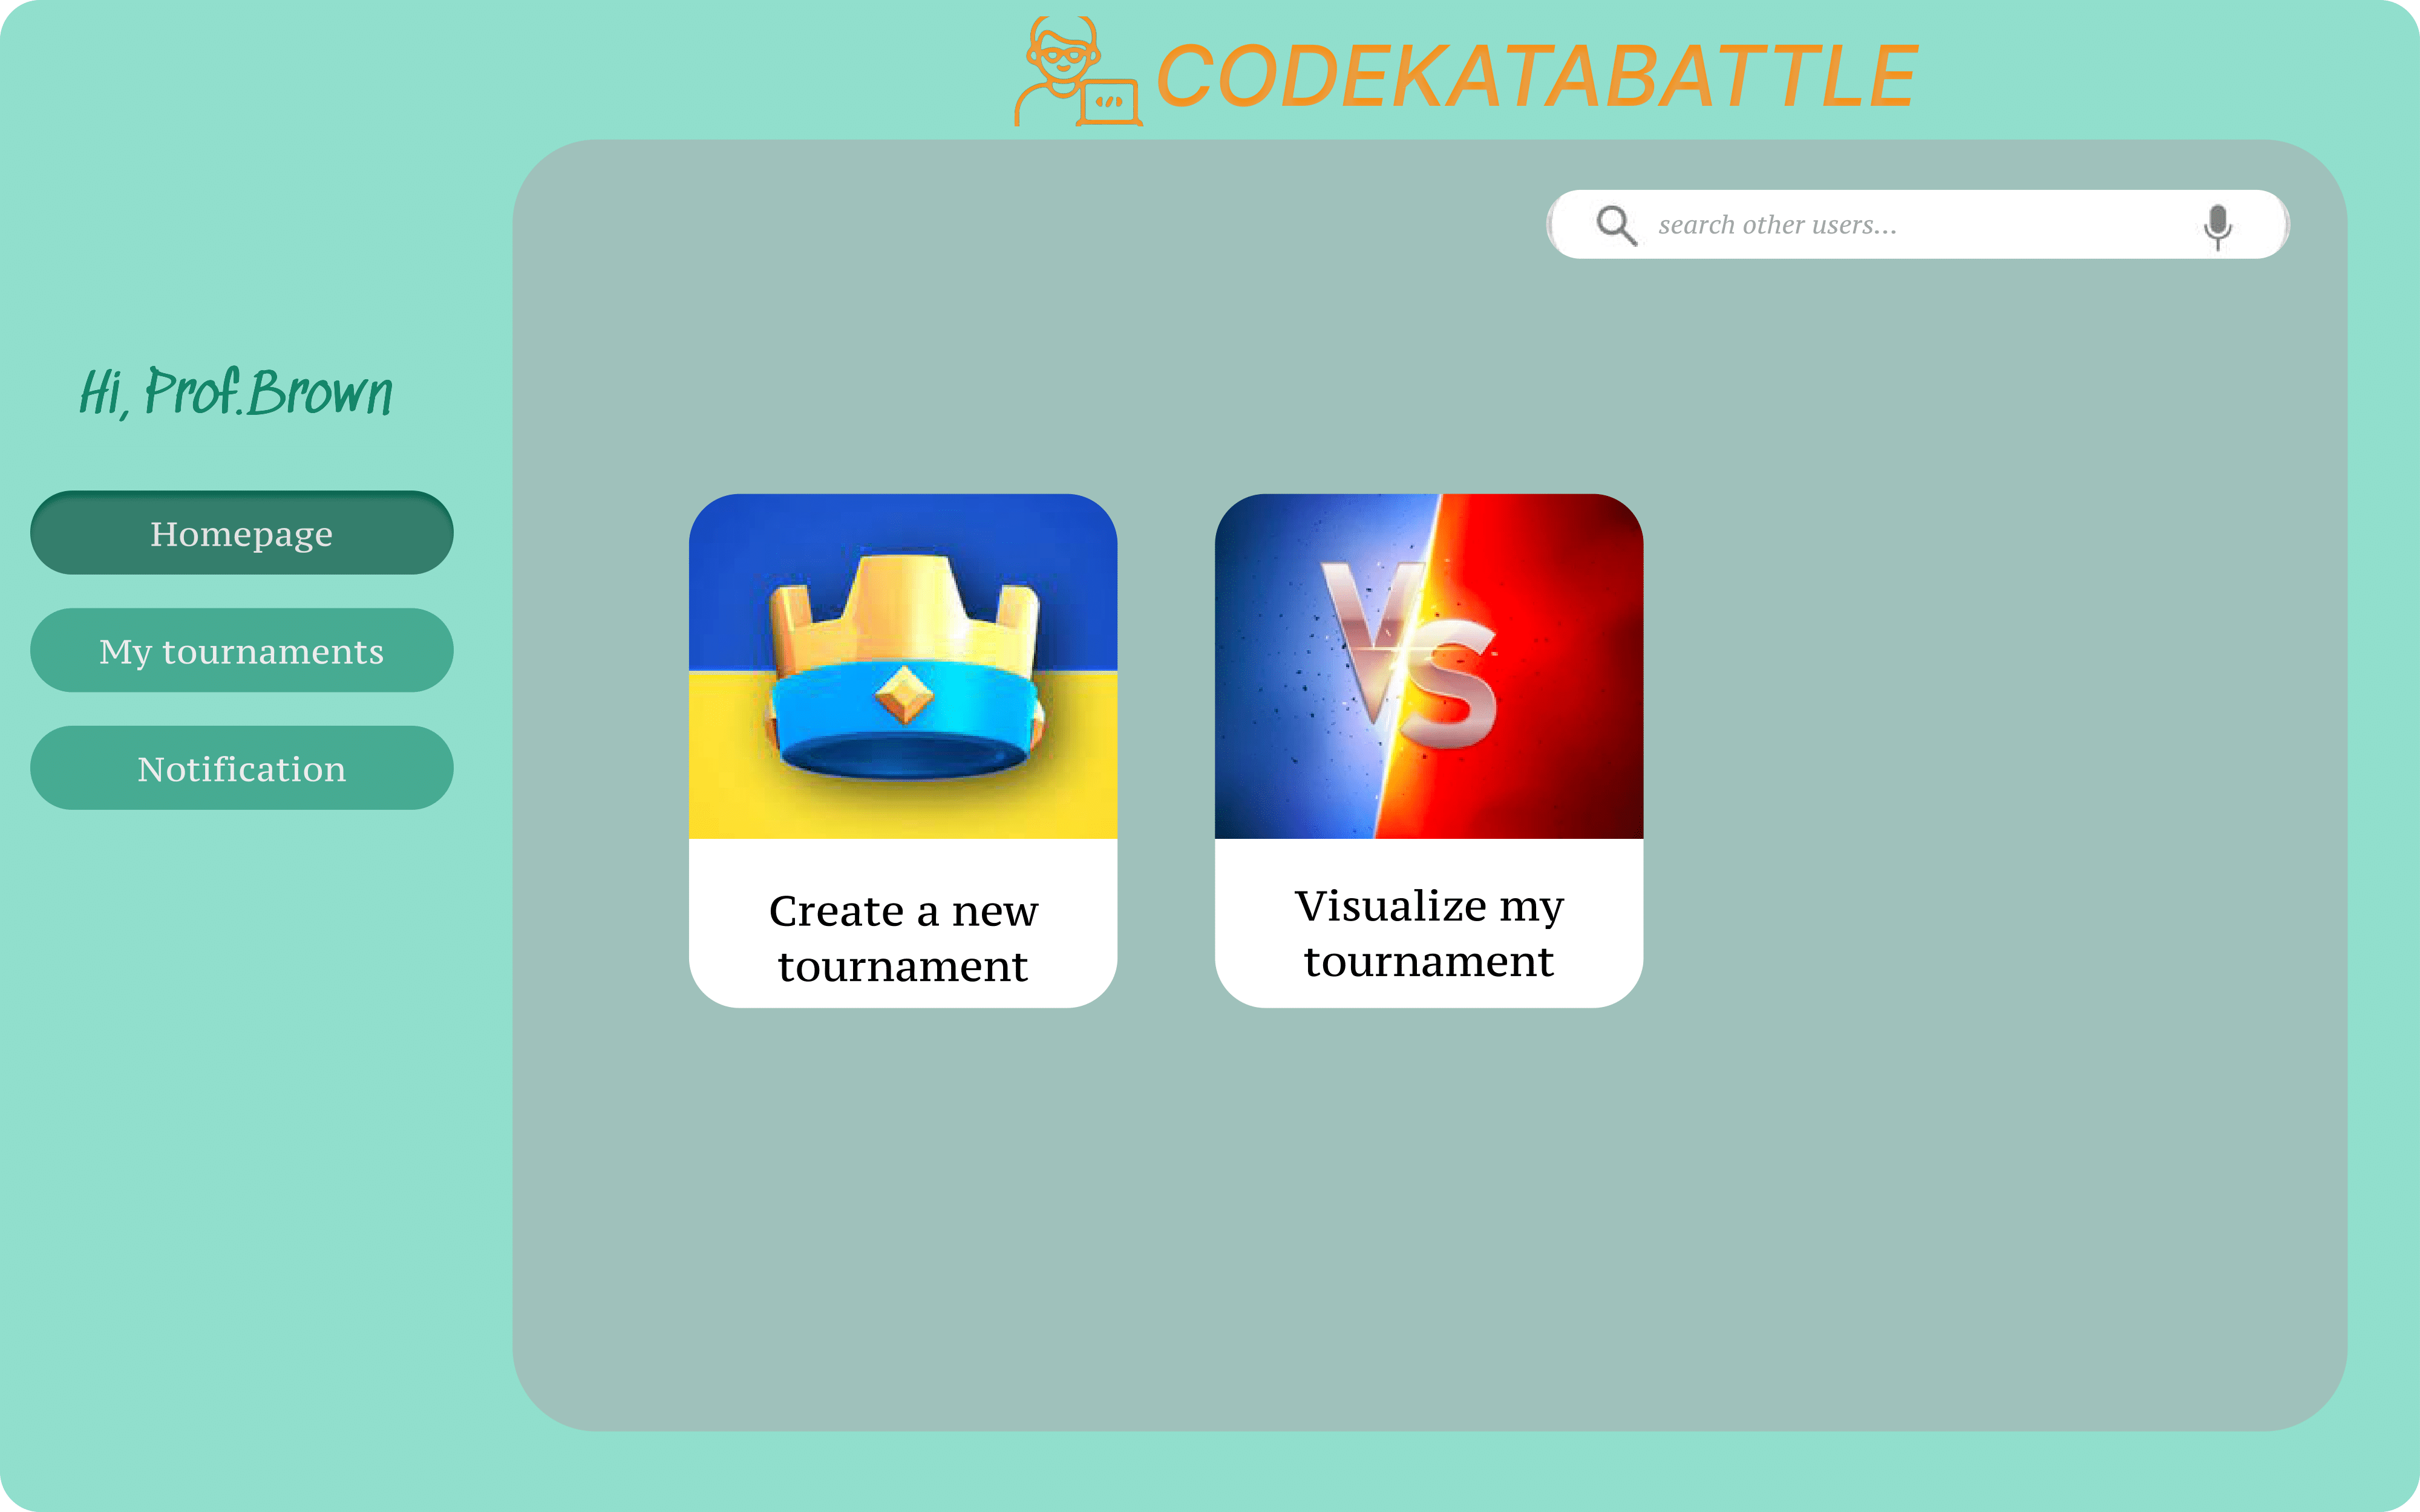
\includegraphics[width=0.8\textwidth]{images/user_interface/UI_sw2-10.png}
    \caption{Educator's homepage}
\end{figure}

\begin{figure}[H]
    \centering
    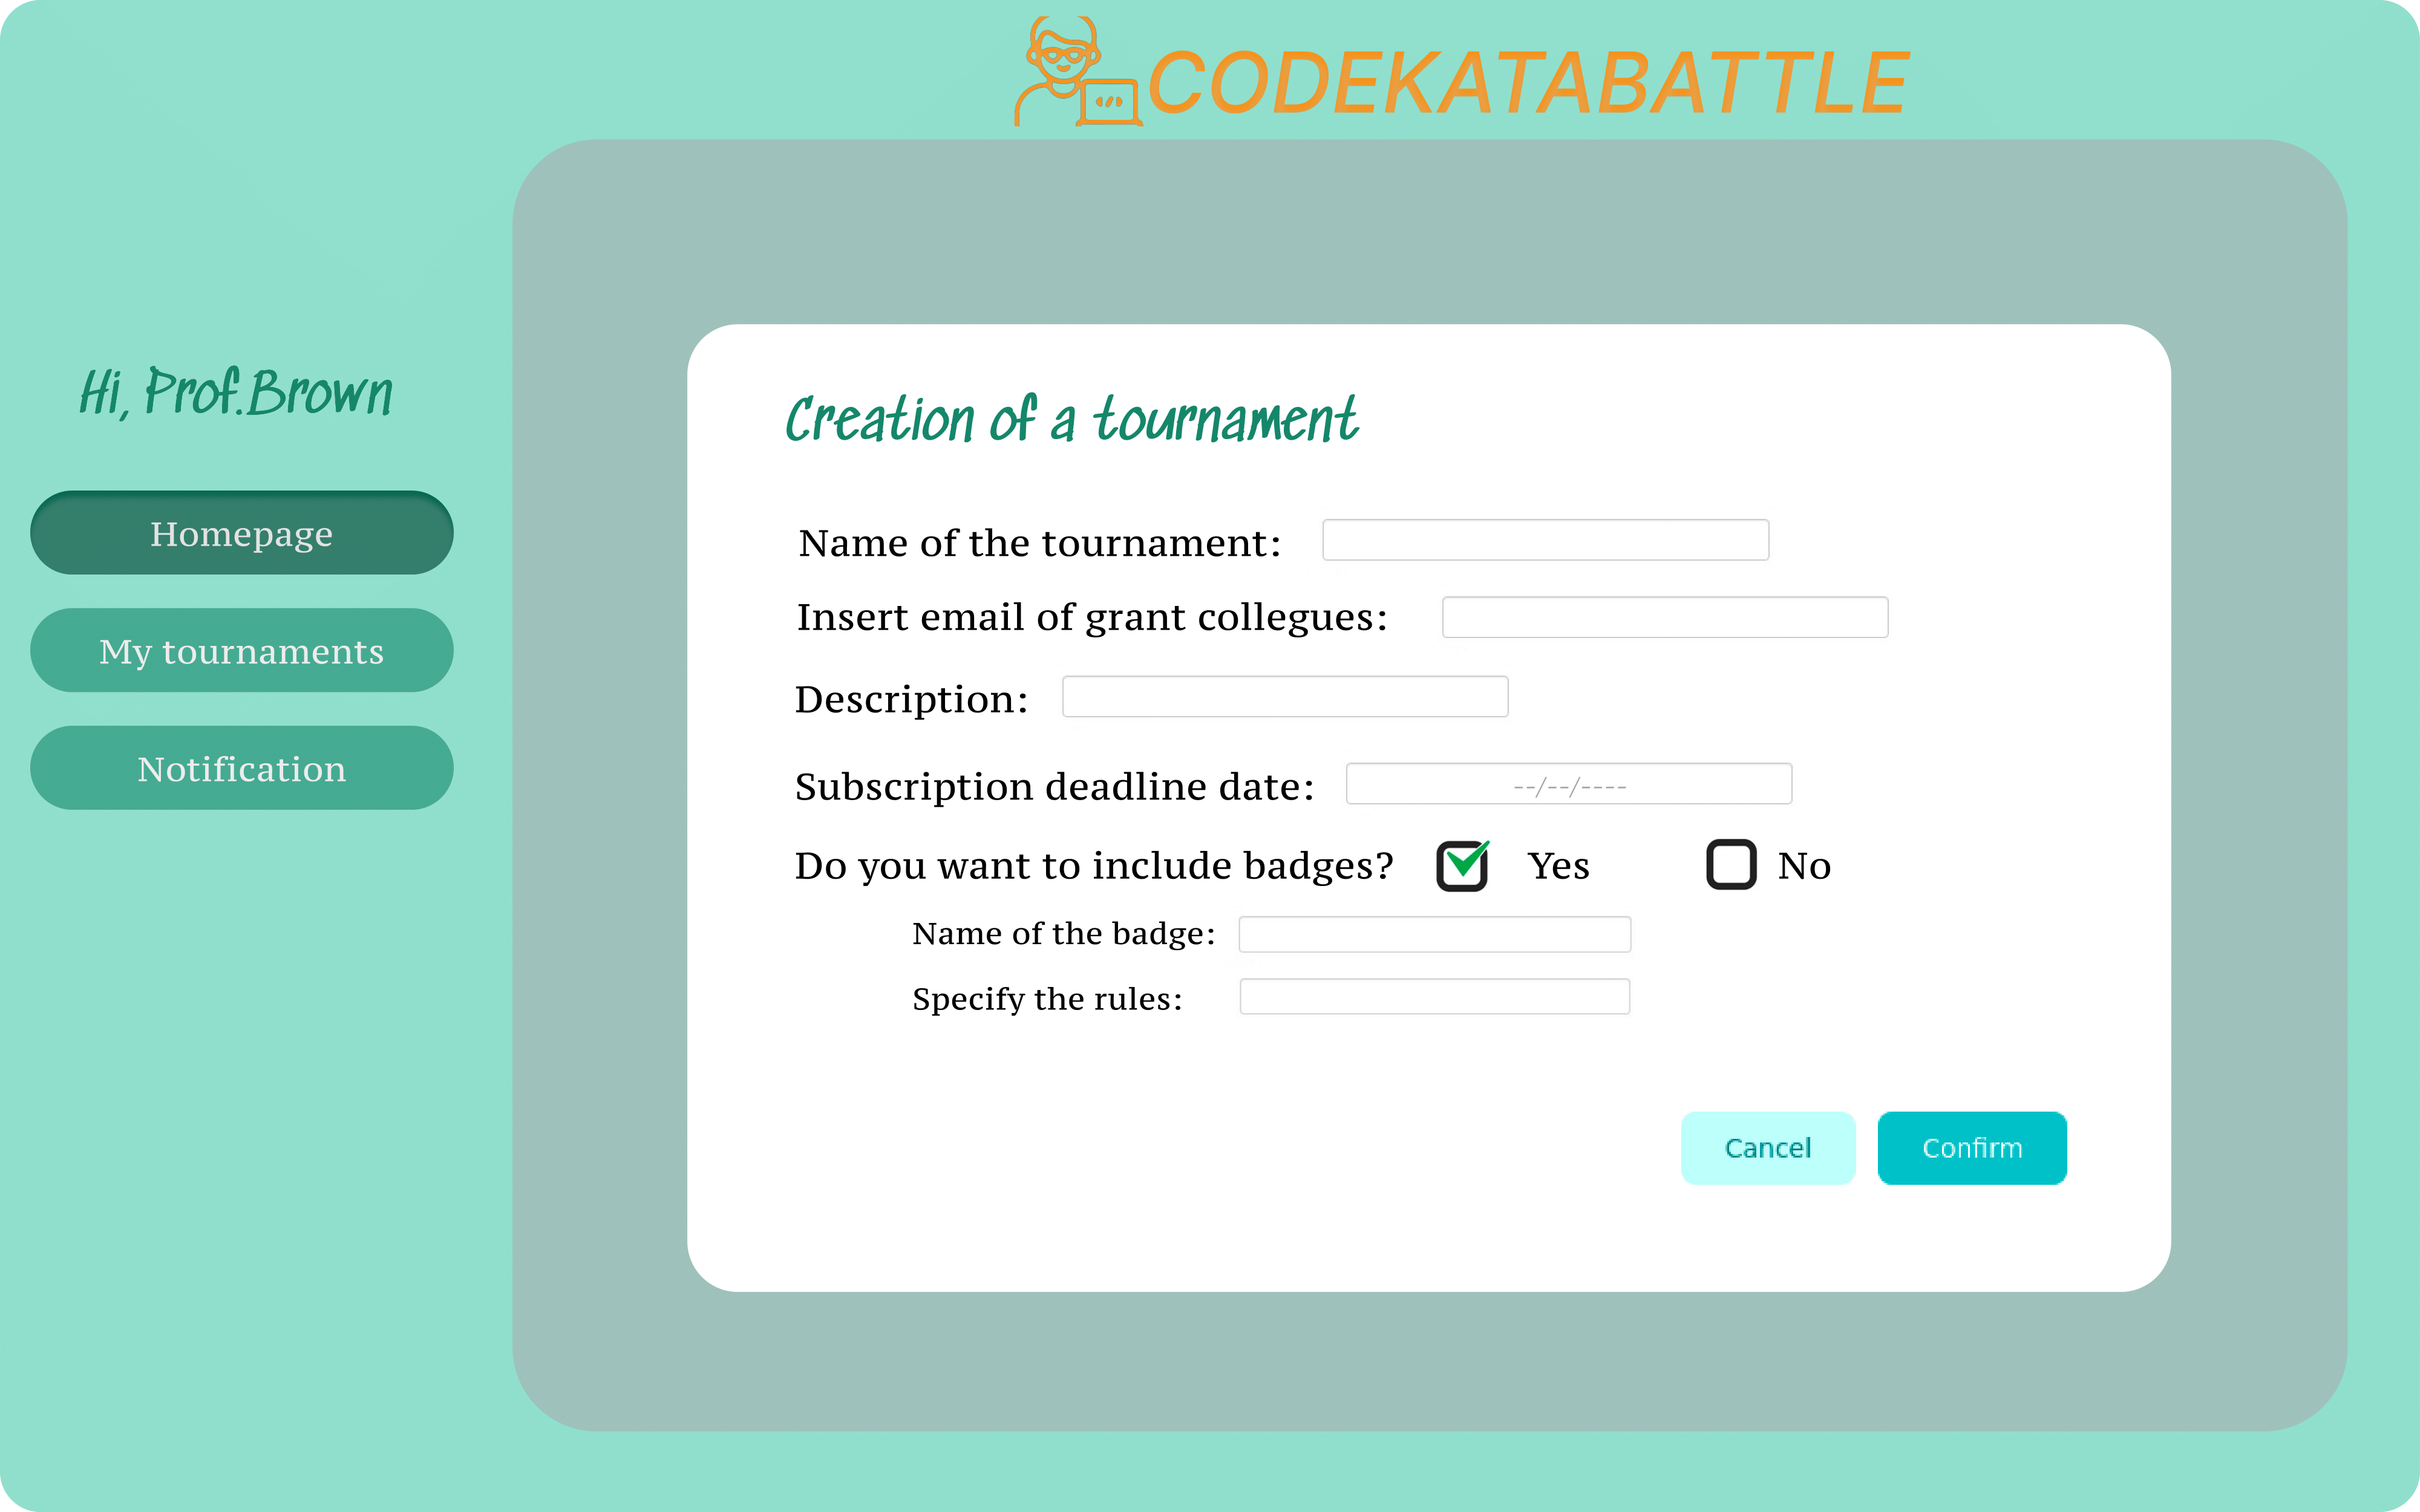
\includegraphics[width=0.8\textwidth]{images/user_interface/UI_sw2-11.png}
    \caption{Creation of a tournament page - educator's page}
\end{figure}

\begin{figure}[H]
    \centering
    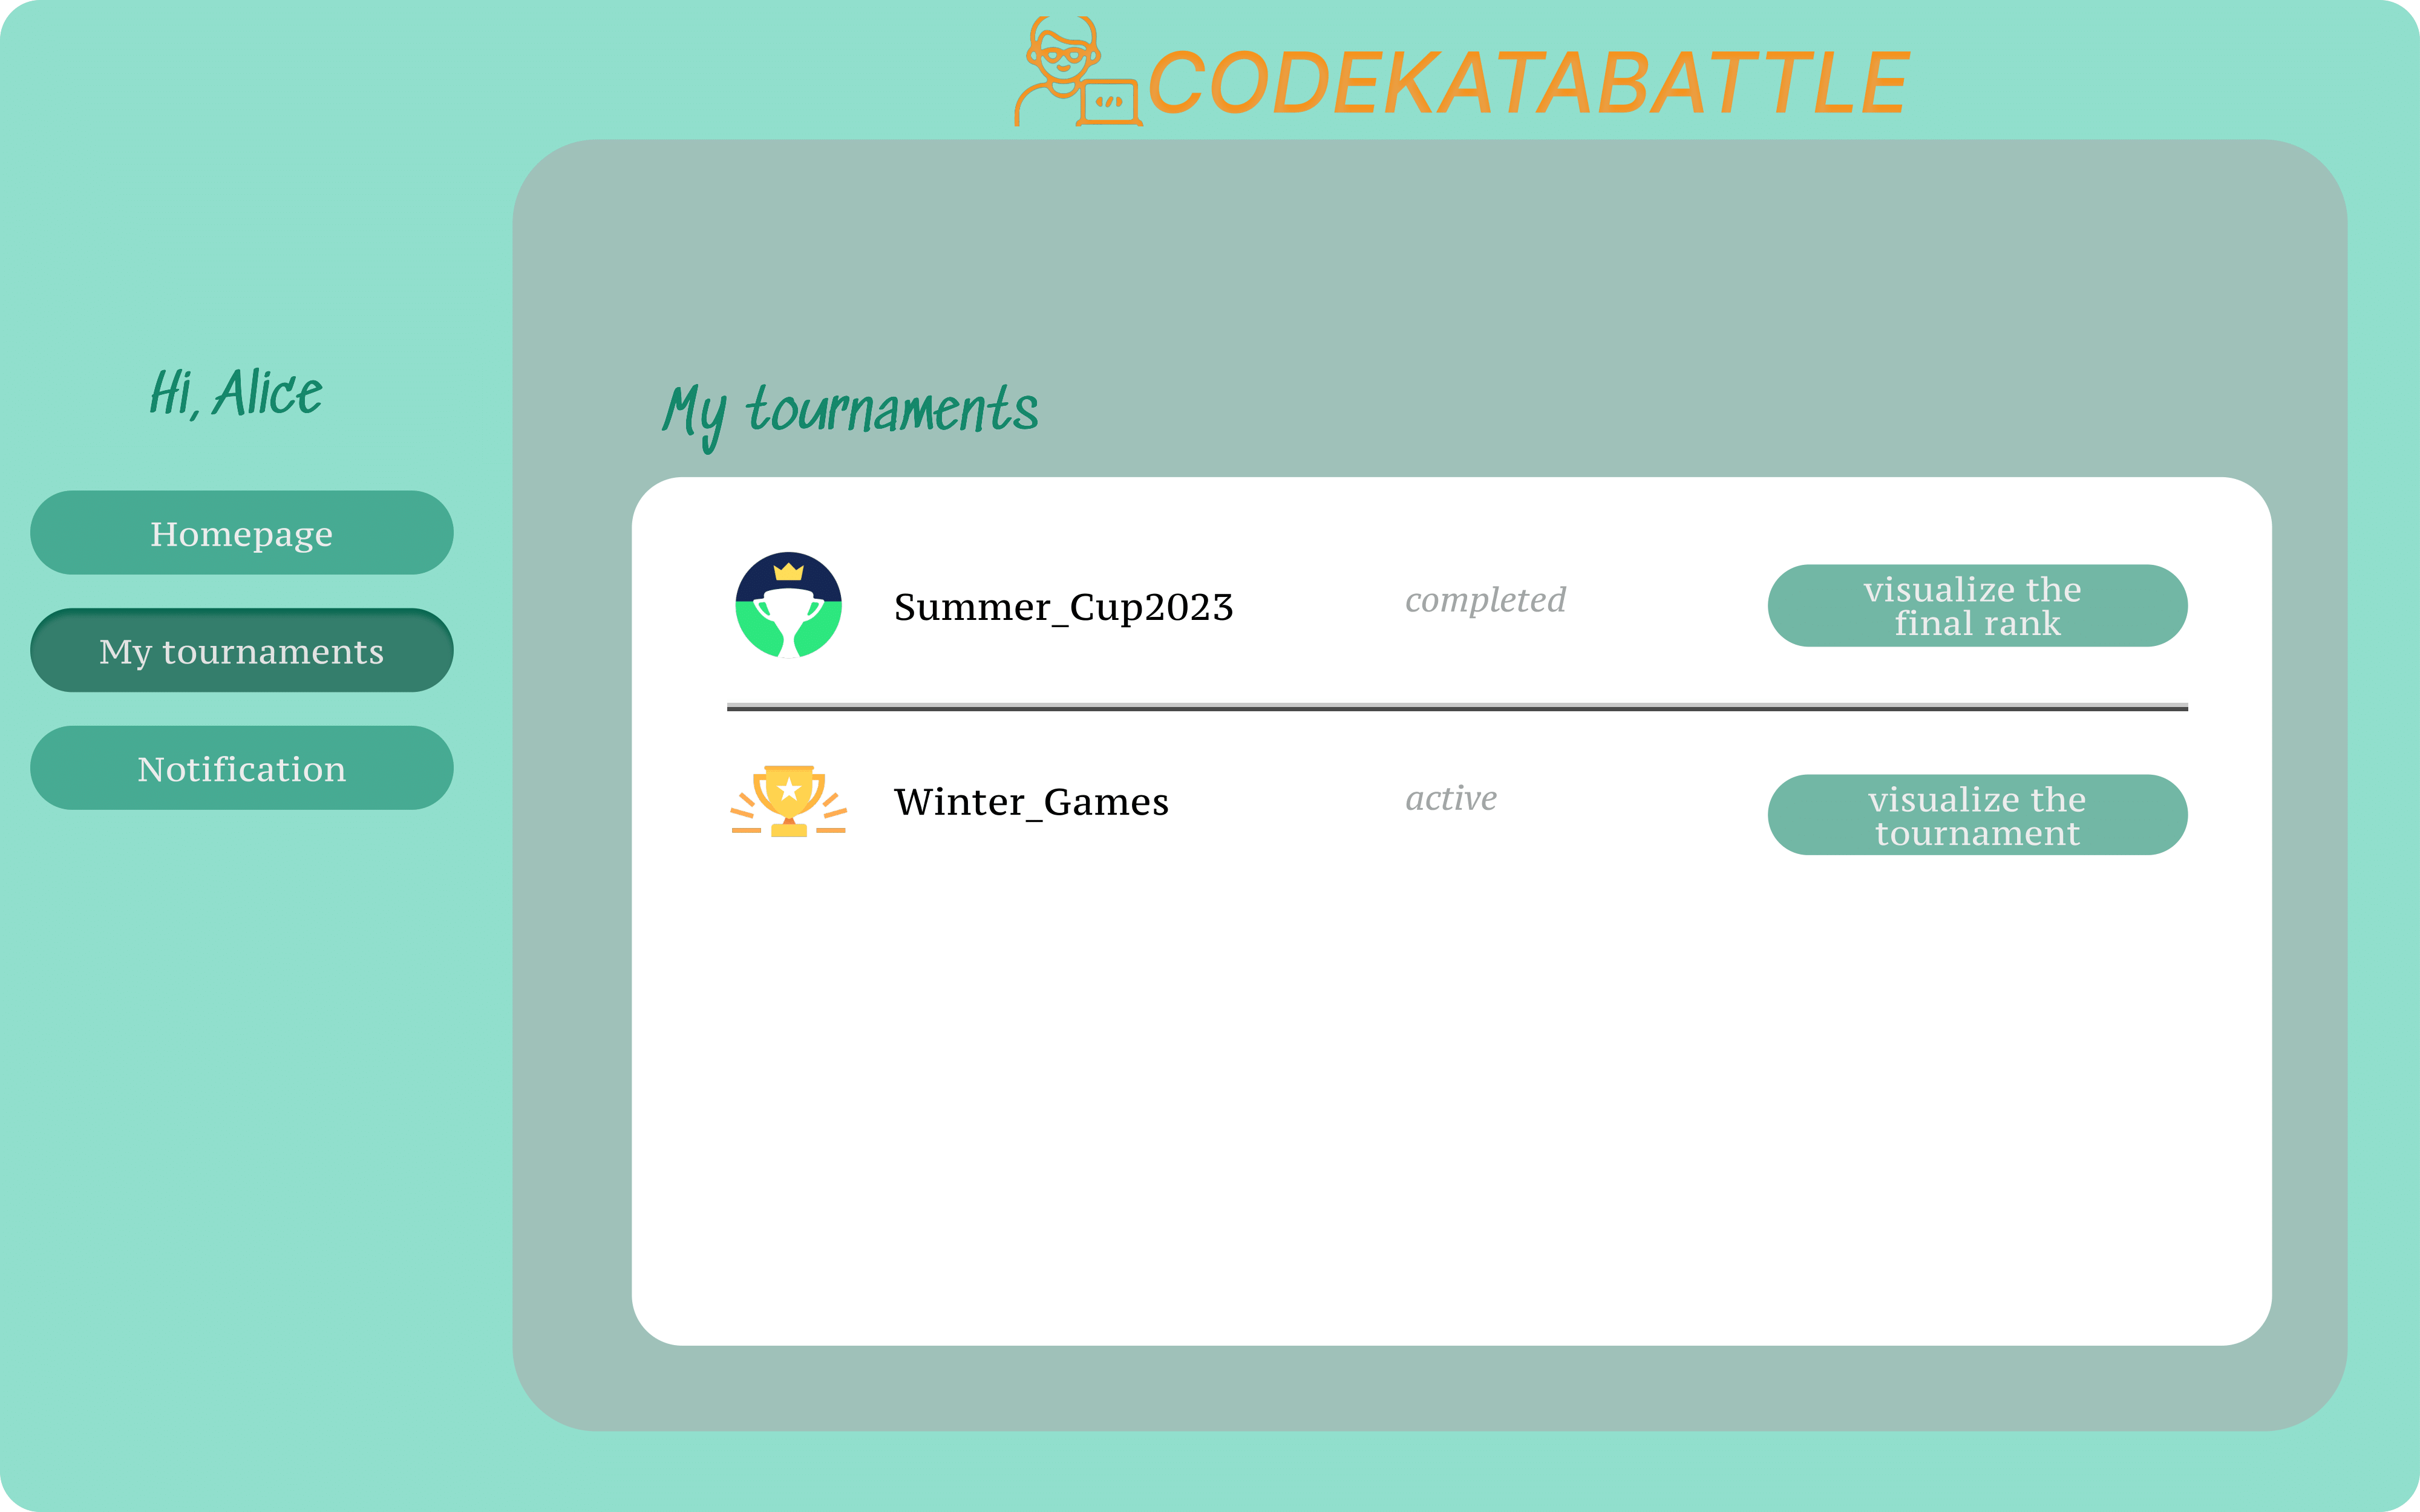
\includegraphics[width=0.8\textwidth]{images/user_interface/UI_sw2-12.png}
    \caption{My tournaments page - educator's page}
\end{figure}

\begin{figure}[H]
    \centering
    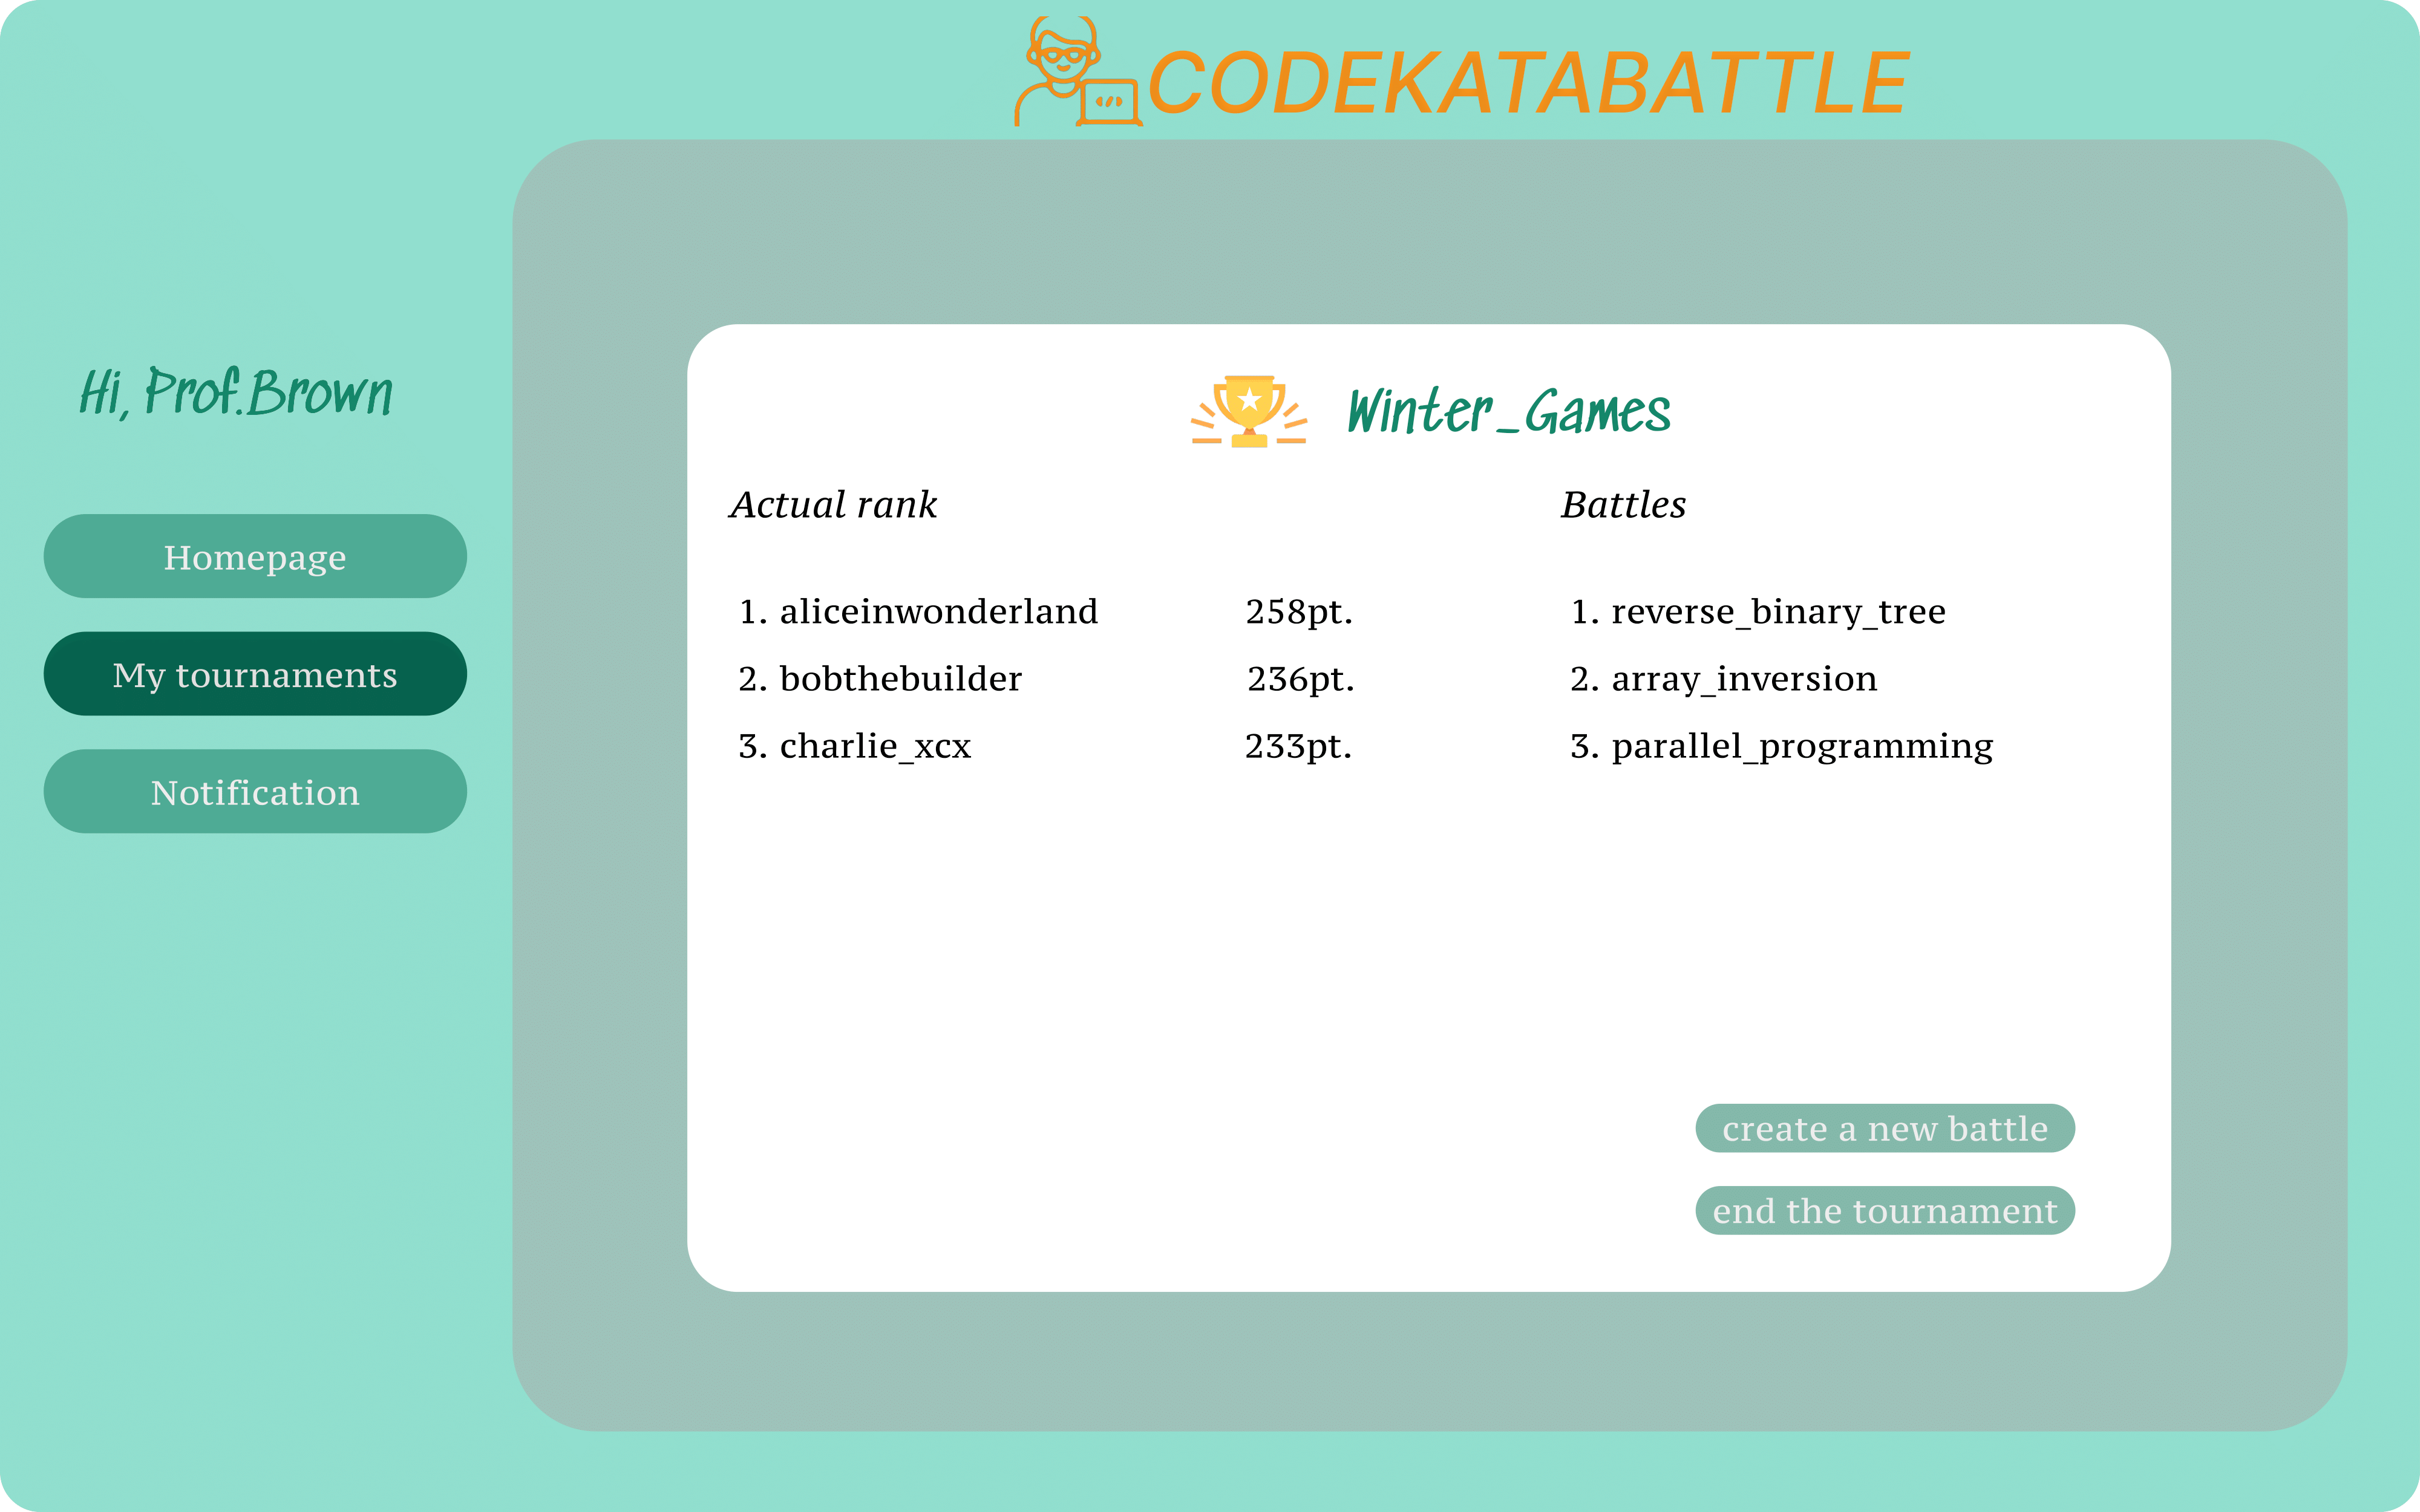
\includegraphics[width=0.8\textwidth]{images/user_interface/UI_sw2-13.png}
    \caption{Tournament's details - educator's page}
\end{figure}

\begin{figure}[H]
    \centering
    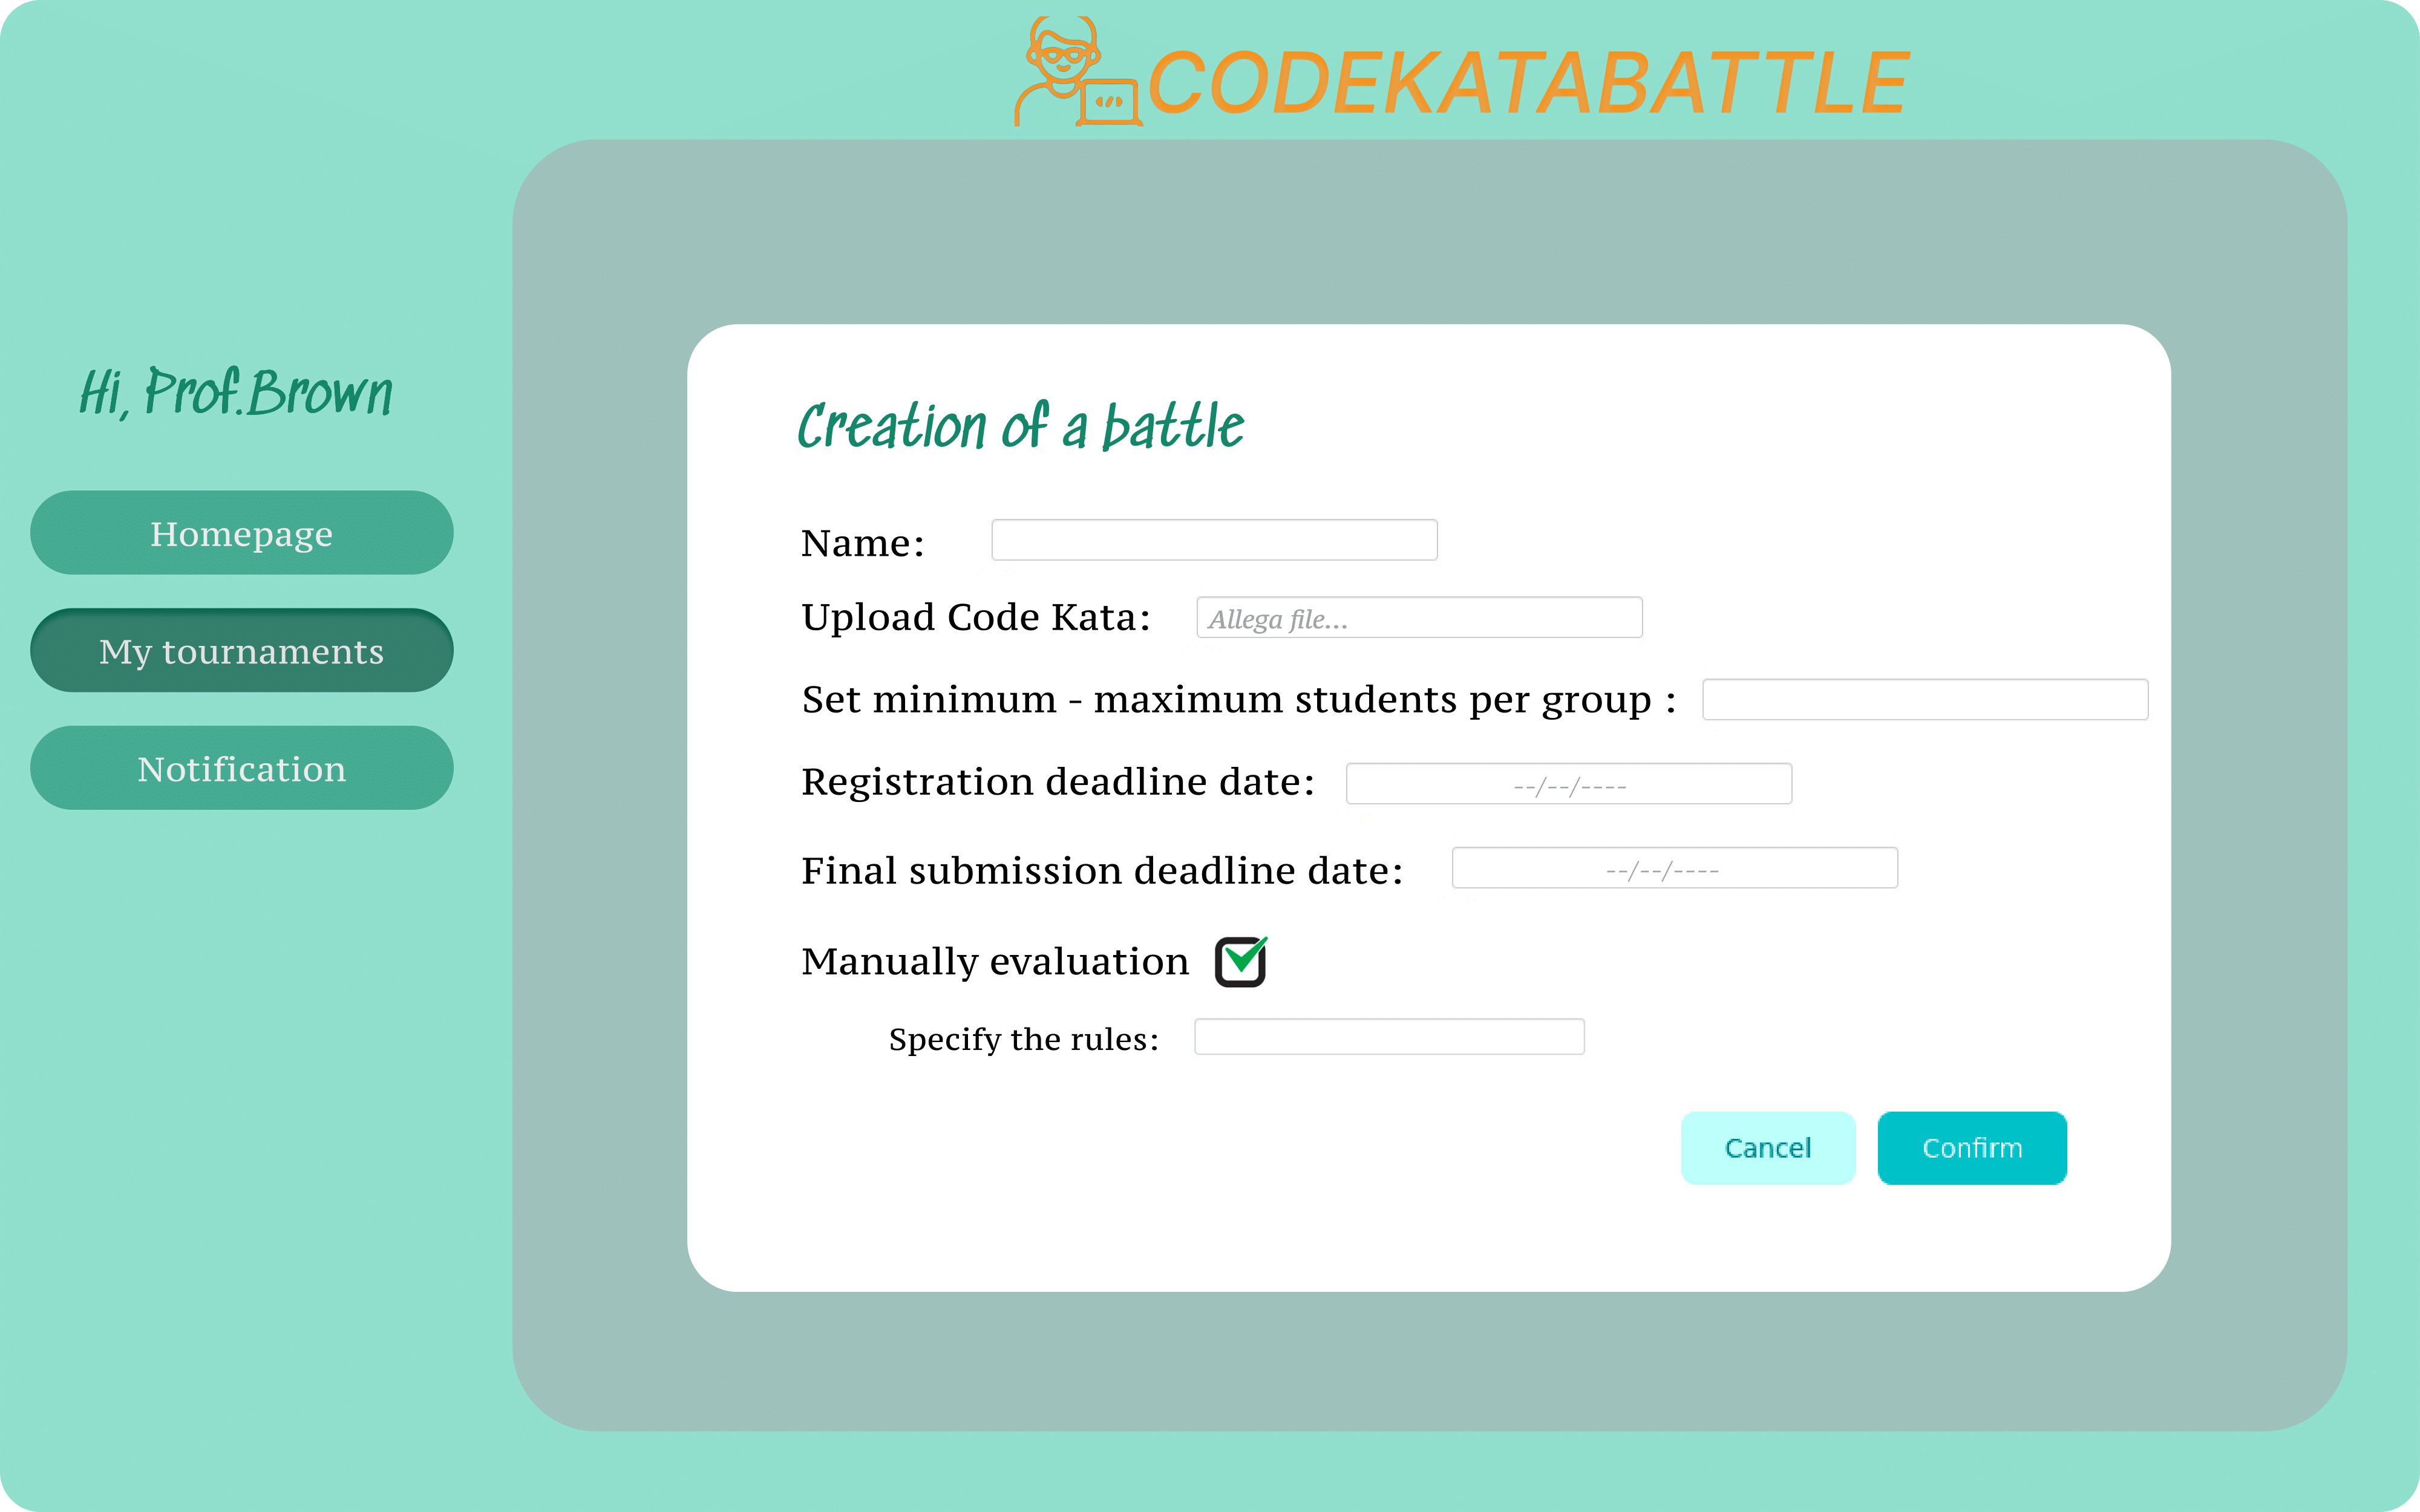
\includegraphics[width=0.8\textwidth]{images/user_interface/UI_sw2-14.png}
    \caption{Creation of a battle page - educator's page}
\end{figure}

\begin{figure}[H]
    \centering
    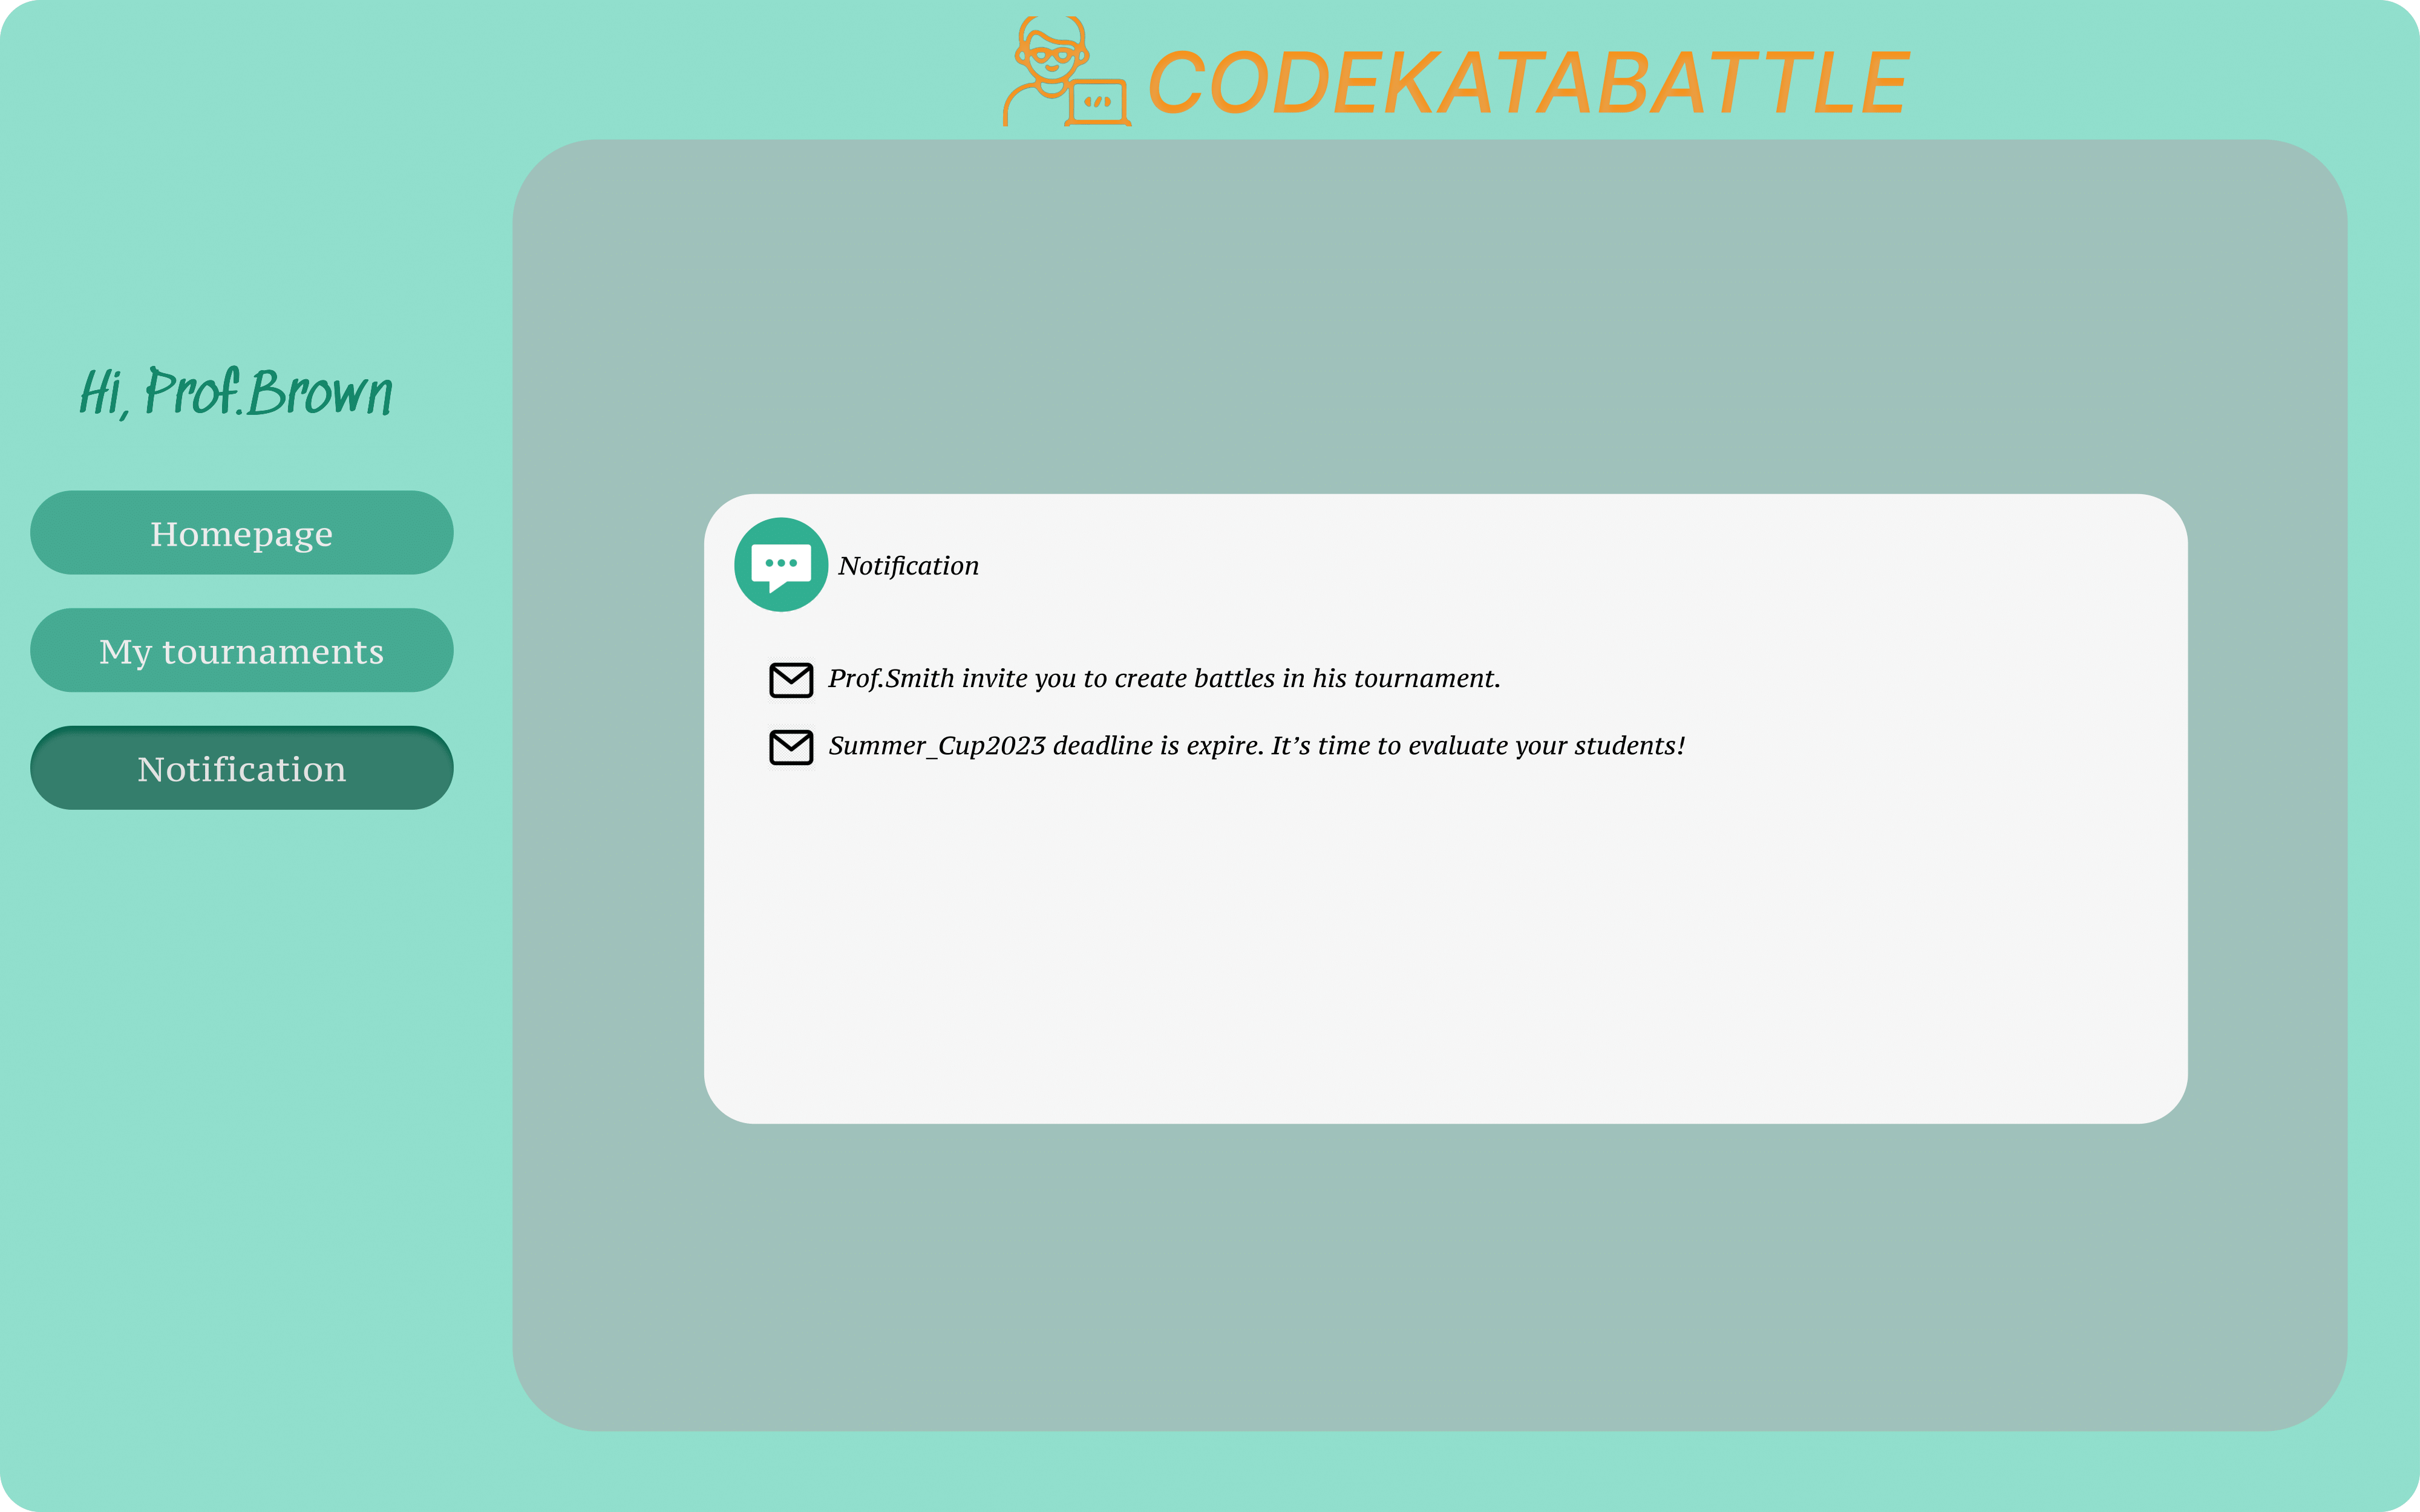
\includegraphics[width=0.8\textwidth]{images/user_interface/UI_sw2-15.png}
    \caption{Notification page - educator's page}
\end{figure}


\subsection{Hardware Interfaces}
This section describes the logical and physical characteristics of each interface 
between the hardware and software componenents of the system.\\
Both educators and students need to have a computer to use the CKB platform.\\
\subsection{Software Interfaces}
This section describes the connections between the system and other specific software components.\\
CodeKataBattle is a web application, so it needs a web browser to be used.\\
\subsection{Communication Interfaces}
This section describes the requirements associated with any communication function required
by this system.\\
All the communications of the eMall infrastructure are made via the HTTP application layer
protocol: obviously, all the devices using the platform must be connected via WiFi or mobile
network (LTE/3G/4G/5G).\\

\section{Functional Requirements}
\subsection{Use Cases Diagrams}
\begin{figure}[H]
    \centering
    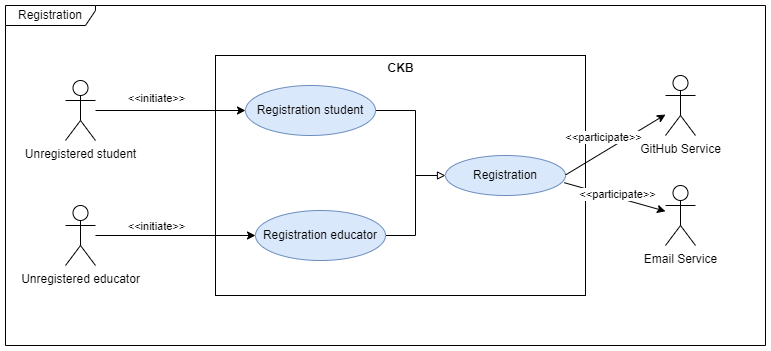
\includegraphics[width=0.8\textwidth]{images/use_cases_diagrams/registration_functions.png}
    \caption{Unregistered user (student or educator) use case diagram}
\end{figure}

\begin{figure}[H]
    \centering
    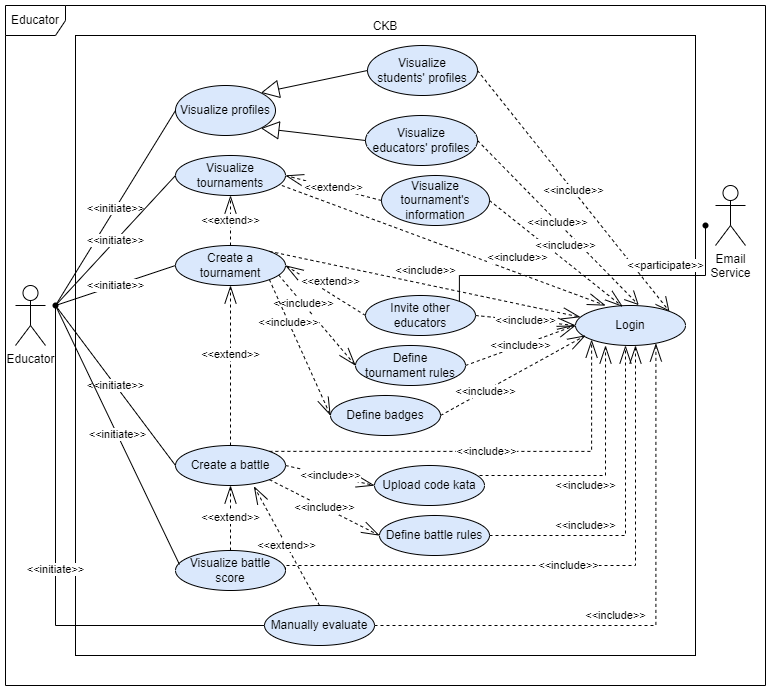
\includegraphics[width=0.8\textwidth]{images/use_cases_diagrams/educators_functions.png}
    \caption{Educator use case diagram}
\end{figure}

\begin{figure}[H]
    \centering
    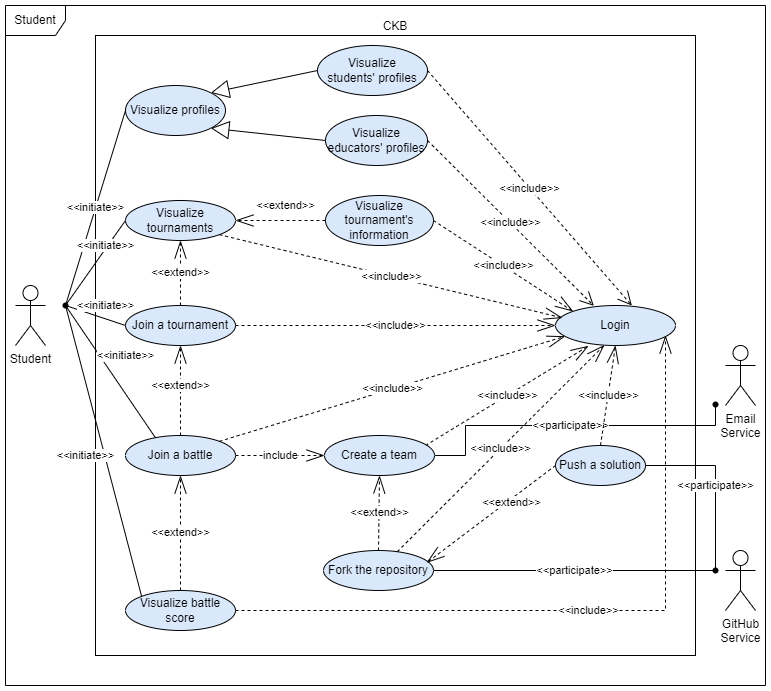
\includegraphics[width=0.8\textwidth]{images/use_cases_diagrams/students_functions.png}
    \caption{Student use case diagram}
\end{figure}
\clearpage

\subsection{Use Cases Description}
\usecase
{1}
{Login}
{Student, Educator}
{The actor is already registered in the system.}
{
    \begin{enumerate}
        \item The actor requires the Login Page.
        \item The system shows the Login Page to the actor.
        \item The actor inserts the credentials (email and passwors) in the form.
        \item The actor submits the form and sends it to the system.
        \item The system processes the information and shows a success message redirecting the user to the homepage.
    \end{enumerate}
}
{The actor is correctly logged in and the homepage is displayed.}
{
    The provided email or password submitted is wrong.
}
{
    In case of exception the system will notify user with a human-readable message.
}
\clearpage

\usecase
{2}
{Registration} % name
{Student, Educator, Email Service, GitHub Service} % actor
{The actor browses and opens the webapp.} % entry condition
{ % event flow
    \begin{enumerate}
        \item The actor clicks the 'Sign up' button.
        \item The actor fills the sign-up form with email and password and submits the form.
        \item The system calls Email Service API to send to the actor an email containing a secret code.
        \item The Email Service sends the email to the actor.
        \item The actor submits the received verification code.
        \item The system displays a success message.
        \item The actor adds his personal information (name, surname, birth date) and submits the form.
        \item The student adds his GitHub username and submits the information.
        \item The system calls GitHub Service API to check if the username is valid.
        \item The GitHub Service sends the response to the system.
        \item The system displays a success message about the verification of GitHub username.
        \item The system processes the provided information and creates a new account.
    \end{enumerate}
}
{The actor signed up correctly.} % exit condition
{ % exceptions
    \begin{enumerate}
        \item A required registration field is missing when the form is submitted.
        \item A provided email is already registered in the system.
        \item A wrong verification code is submitted.
        \item A wrong GitHub username is submitted.
    \end{enumerate}
}
{ % notes
In case of exception the system will notify user with a human-readable message.
}

\usecase
{3}
{Tournament creation}
{Educator, Email Service}
{The actor is already logged in the system.}
{
    \begin{enumerate}
        \item The educator requires the "Create a new tournament" page.
        \item The system shows the "Create a new tournament" page to the educator.
        \item The educator fills the form with tournament name, description and deadline.
        \item The educator can choose to define a set of badges that can be earned by the students.
        \item The educator can invite other educators to join the tournament, giving them the possibility to create battles.
        \item The system sends an email to the invited educators.
    \end{enumerate}
}
{The tournament is created and the tournament page is shown.}
{
    \begin{itemize}
        \item The educator provides an invalid name or description.
        \item The educator provides a deadline that is not in the future.
        \item The educator provides an invalid email.
    \end{itemize}
}
{
    In case of exception the system will notify user with a human-readable message.
}

\clearpage

\usecase
{4}
{Battle creation}
{Educator, Student, Email Service}
{The authorized educator is in the tournament page.}
{
    \begin{enumerate}
        \item The educator requires the "Create a battle" page.
        \item The system shows the "Create a battle" page to the educator.
        \item The educator gives a name to the tournament.
        \item The educator uploads the code kata.
        \item The educator sets the minimum and maximum number of group members.
        \item The educator sets a deadline to subscribe to the tournament.
        \item The educator sets a deadline to submit the solutions.
        \item The educator can choose to include a manual evaluation of the students' work.
        \item The system sends an email to all the students that are subscribed to the tournament.
    \end{enumerate}
}
{The battle is created and the battle page is shown.}
{
    \begin{itemize}
        \item The educator provides an invalid name.
        \item The system does not upload a code kata.
        \item The educator provides an invalid number of group members.
        \item The educator provides a deadline that is not in the future.
    \end{itemize}
}
{
    In case of exception the system will notify user with a human-readable message.
}


\clearpage

\usecase
{5}
{Tournament visualization}
{Educator, Student}
{The actor is already logged in the system.}
{
    \begin{enumerate}
        \item The actor requires the "Ongoing tournaments" page.
        \item The system shows the "Ongoing tournaments" page to the actor.
        \item The actor selects a tournament.
    \end{enumerate}
}
{The tournament page is shown.}
{
    None.
}
{}


\usecase
{6}
{Joining a tournament}
{Student, Email Service}
{The authorized student is in the tournament page.}
{
    \begin{enumerate}
        \item The student clicks "Join a tournament" button.
        \item The system signs up the student to the tournament.
        \item The system sends an email to the student.
    \end{enumerate}
}
{The tournament page is shown.}
{
    None.
}
{}

\clearpage

\usecase
{7.1}
{Joining a battle - Singleton}
{Student, Email Service}
{The authorized student is in the tournament page and the battle allows singleton groups.}
{
    \begin{enumerate}
        \item The student clicks the "Join" button corresponding to the battle.
        \item The system shows a form to join the battle.
        \item The student fills the form as a singleton.
        \item The system signs up the student to the battle.
        \item The system sends an email to the student.
    \end{enumerate}
}
{The tournament page is shown.}
{
    None.
}
{}

\clearpage

\usecase
{7.2}
{Joining a battle - Creating a group}
{Student, Email Service}
{The authorized student is in the tournament page.}
{
    \begin{enumerate}
        \item The student clicks the "Join" button corresponding to the battle.
        \item The system shows a form to join the battle.
        \item The student fills the form with other students' email and clicks the "Create group" button.
        \item The system creates the team but does not sign it up to the battle yet.
        \item The system sends an email to the students.
    \end{enumerate}
}
{The tournament page is shown.}
{
    \begin{enumerate}
        \item The student does not provide valid emails.
        \item The student does not provide a valid number of emails.
    \end{enumerate}

}
{
    In case of exception the system will notify user with a human-readable message.
}

\clearpage

\usecase
{7.3}
{Joining a battle - Joining a group}
{Student, EmailProvider}
{The authorized student is logged in the system.}
{
    \begin{enumerate}
        \item The student requires the "Notification" page.
        \item The system shows the "Notification" page to the student.
        \item The student selects an invite.
        \item The student clicks the "Join" button.
        \item The system updates the group.
        \item If constraints are met, the system signs up the group to the battle.
        \item The system sends an email to the student.
    \end{enumerate}
}
{The tournament page is shown.}
{
    The battle registration deadline has expired.
}
{
    In case of exception the system will notify user with a human-readable message.
}


\usecase
{8}
{Battle execution}
{Student, GitHub Service}
{The student has received the email with the link to the code kata repository.}
{
    \begin{enumerate}
        \item The student forks the code kata repository.
        \item The student sets up the automated workflow on GitHub Actions.
        \item The student pushes his code to the repository.
    \end{enumerate}
}
{The system performs the automated evaluation and updates the battle score.}
{
    The battle submission deadline has expired.
}
{
    In case of exception the system will notify user with a human-readable message.
}

\usecase
{9}
{Evaluation} % name
{Student, Educator, GitHub Service} % actor
{The student has committed the code.} % entry condition
{ % event flow
    \begin{enumerate}
        \item The student pushes the code to GitHub.
        \item The GitHub service notify the system about the new push.
        \item The system pulls the code from GitHub service.
        \item The GitHub service provides the requested code to the system.
        \item The system makes the automatic evaluation.
        \item The system sets the calcutaed score to the code.
        \item The system notify via email the student about the evaluation and the score assigned to his code.
        \item The educator can get the code from the system.
        \item The system provides the code to the educator.
        \item The educator can manually evaluate the code at the end of the battle and set a score.
        \item The system updates the score.
    \end{enumerate}
}
{The system sends an email to the students.} % exit condition
{ % exceptions
 None. 
}
{ % notes
}
\clearpage

\usecase
{10}
{Conclusion of a battle}
{Student, Email Service}
{The submission deadline (and, if required, the manual evaluation stage) has expired.}
{
    \begin{enumerate}
        \item The system updates the tournament score and rank.
        \item The system sends an email to the students.
    \end{enumerate}
}
{The battle is closed.}
{
    None.
}
{}


\usecase
{11}
{Conclusion of a tournament}
{Educator, Student, Email Service}
{The authorized educator is in the tournament page.}
{
    \begin{enumerate}
        \item The educator closes the tournament.
        \item The system awards badges to the students.
        \item The system sends an email to the students.
    \end{enumerate}
}
{The tournament is closed.}
{
    None.
}
{}

\clearpage

\usecase
{12}
{Profile visualization} % name
{Student, Educator} % actor
{The actor is logged in the system.} % entry condition
{ % event flow
    \begin{enumerate}
        \item The actor searches a student profile.
        \item The system returns the selected student profile.
    \end{enumerate}
}
{The actor visualizes the personal information of the student.} % exit condition
{ % exceptions
 The selected profile does not exist. 
}
{ % notes
In case of exception the system will notify user with a human-readable message.
}

\subsection{Sequence Diagrams}
\begin{figure}[H]
    \centering
    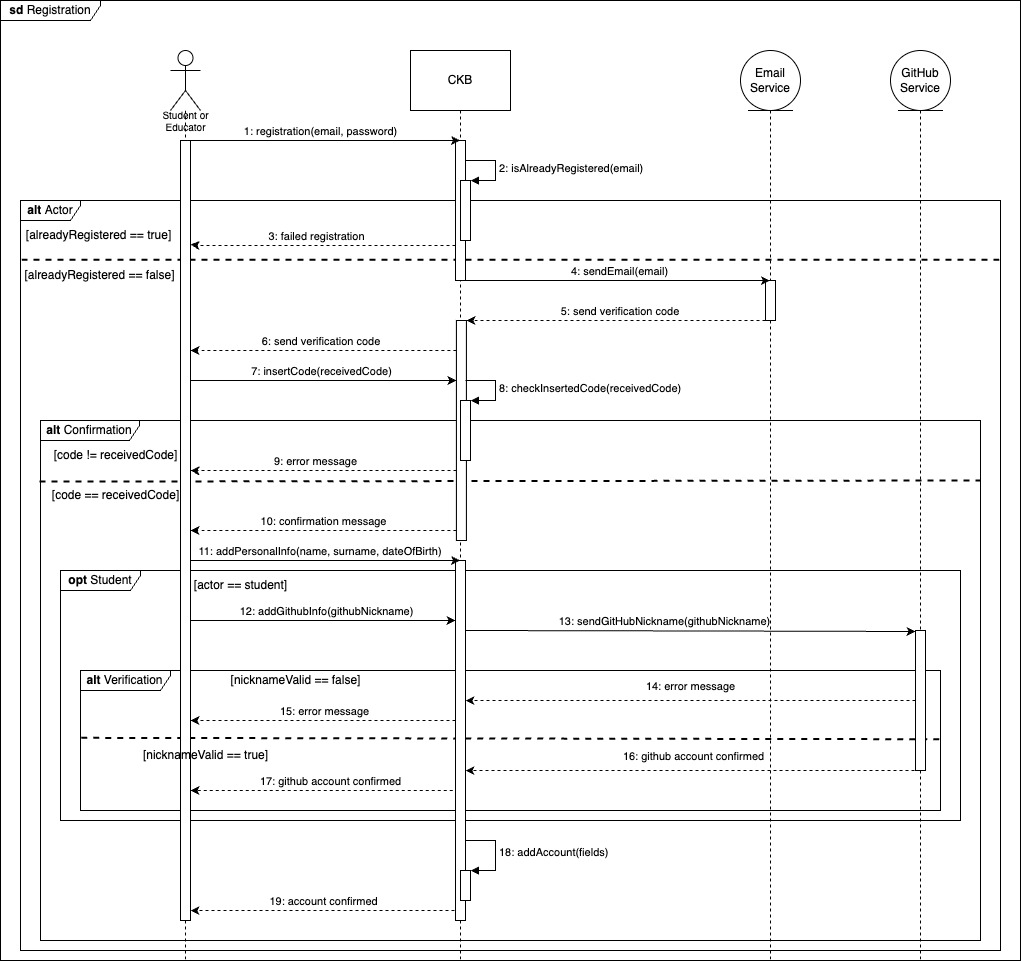
\includegraphics[width=0.95\textwidth]{images/seq_diagrams/Registration.jpg}
    \caption{Registration sequence diagram}
\end{figure}
\clearpage

\begin{figure}[H]
    \centering
    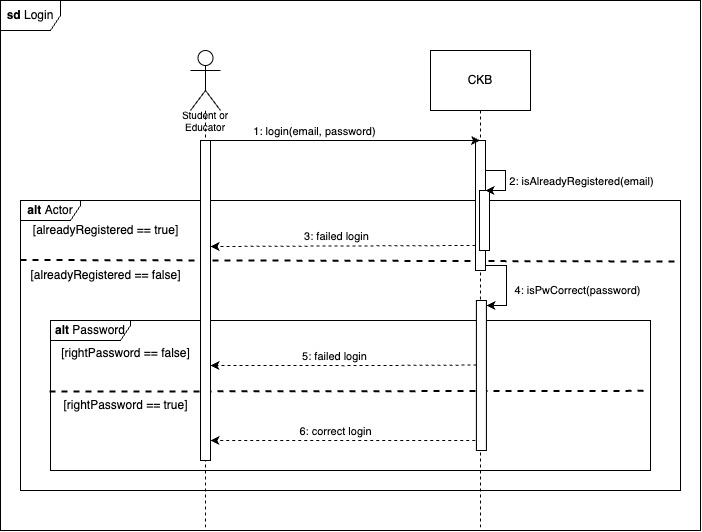
\includegraphics[width=0.95\textwidth]{images/seq_diagrams/Login.jpg}
    \caption{Login sequence diagram}
\end{figure}
\clearpage

\begin{figure}[H]
    \centering
    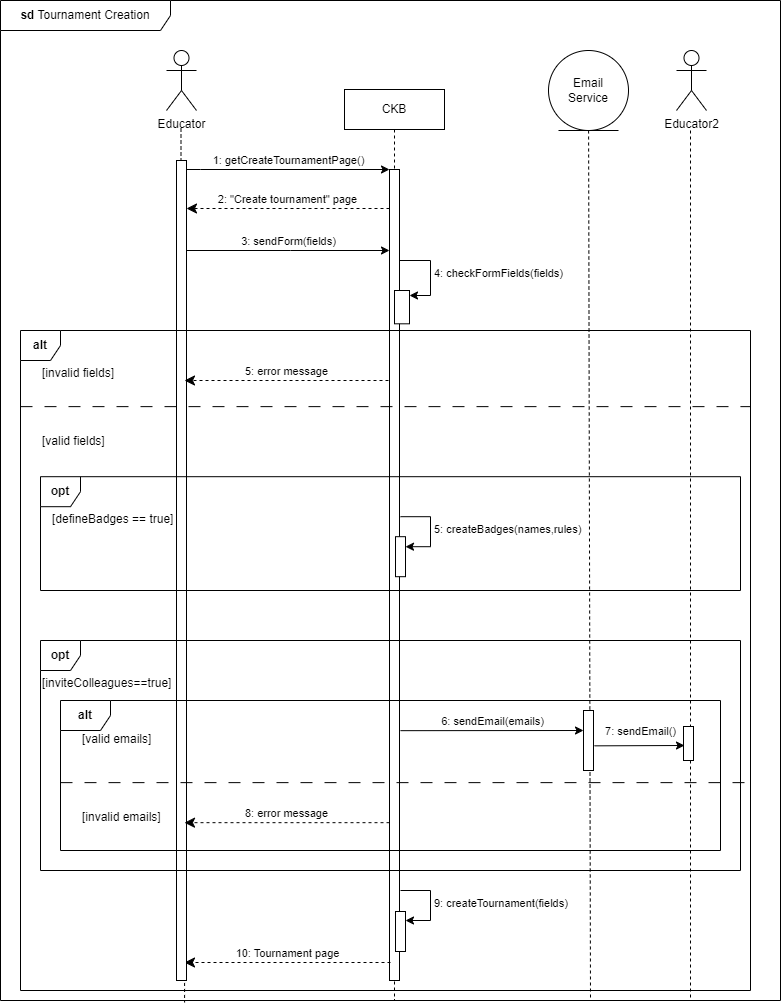
\includegraphics[width=0.95\textwidth]{images/seq_diagrams/tournament_creation.png}
    \caption{Tournament creation sequence diagram}
\end{figure}
\clearpage

\begin{figure}[H]
    \centering
    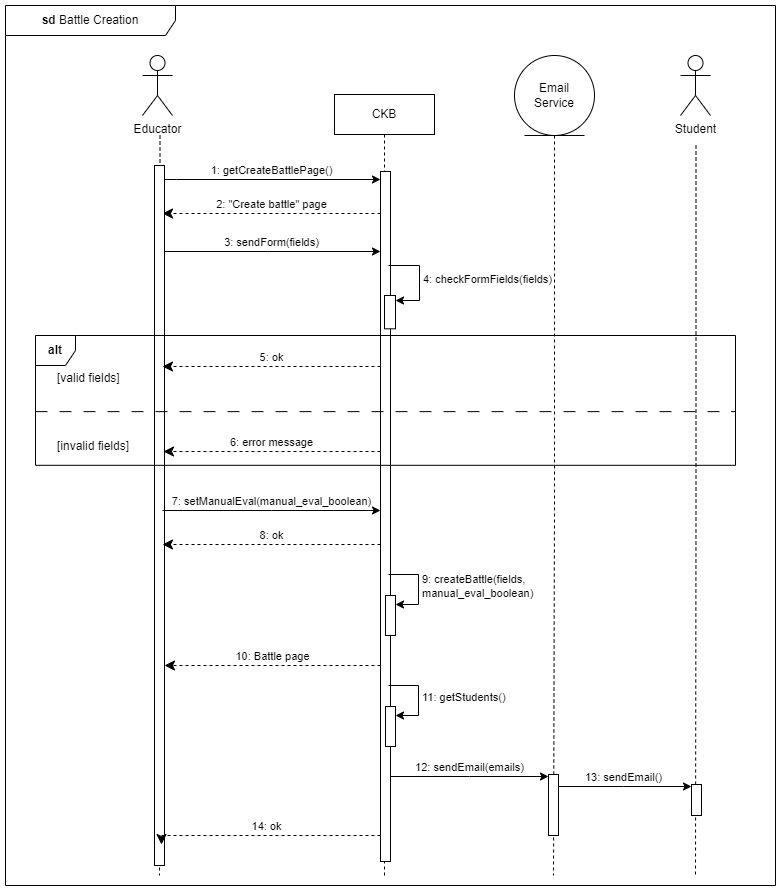
\includegraphics[width=0.95\textwidth]{images/seq_diagrams/battle_creation.png}
    \caption{Battle creation sequence diagram}
\end{figure}
\clearpage

\begin{figure}[H]
    \centering
    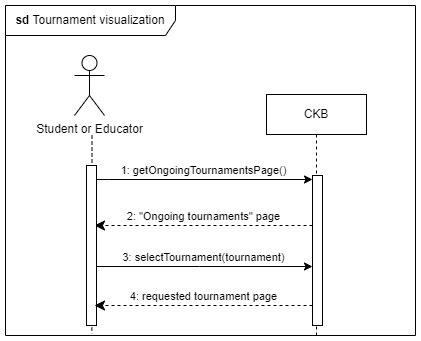
\includegraphics[width=0.95\textwidth]{images/seq_diagrams/tournament_visualization.png}
    \caption{Tournament visualization sequence diagram}
\end{figure}
\clearpage

\begin{figure}[H]
    \centering
    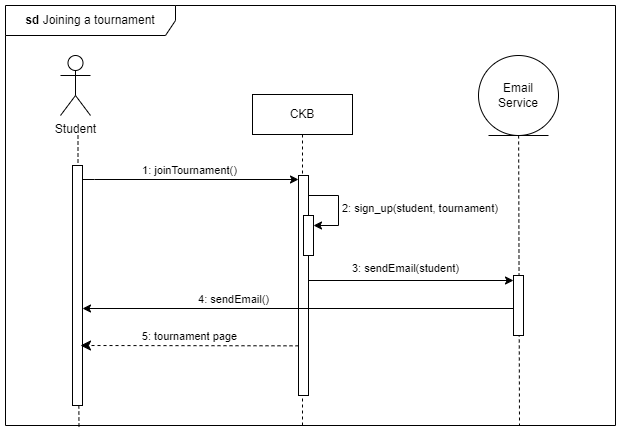
\includegraphics[width=0.95\textwidth]{images/seq_diagrams/joining_tournament.png}
    \caption{Joining a tournament sequence diagram}
\end{figure}
\clearpage

\begin{figure}[H]
    \centering
    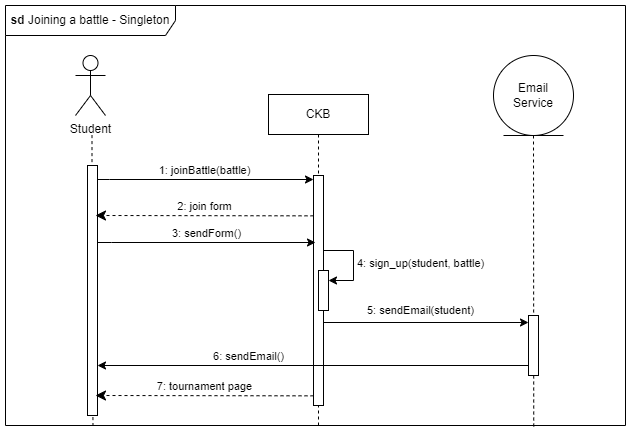
\includegraphics[width=0.95\textwidth]{images/seq_diagrams/joining_battle-singleton.png}
    \caption{Joining a battle as a singleton sequence diagram}
\end{figure}
\clearpage

\begin{figure}[H]
    \centering
    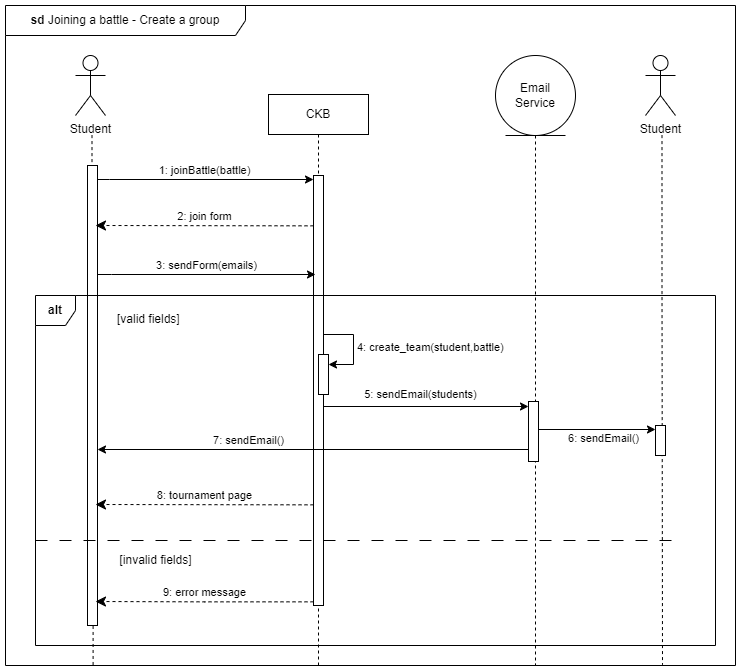
\includegraphics[width=0.95\textwidth]{images/seq_diagrams/joining_battle-create_group.png}
    \caption{Joining a battle by creating a group sequence diagram}
\end{figure}
\clearpage

\begin{figure}[H]
    \centering
    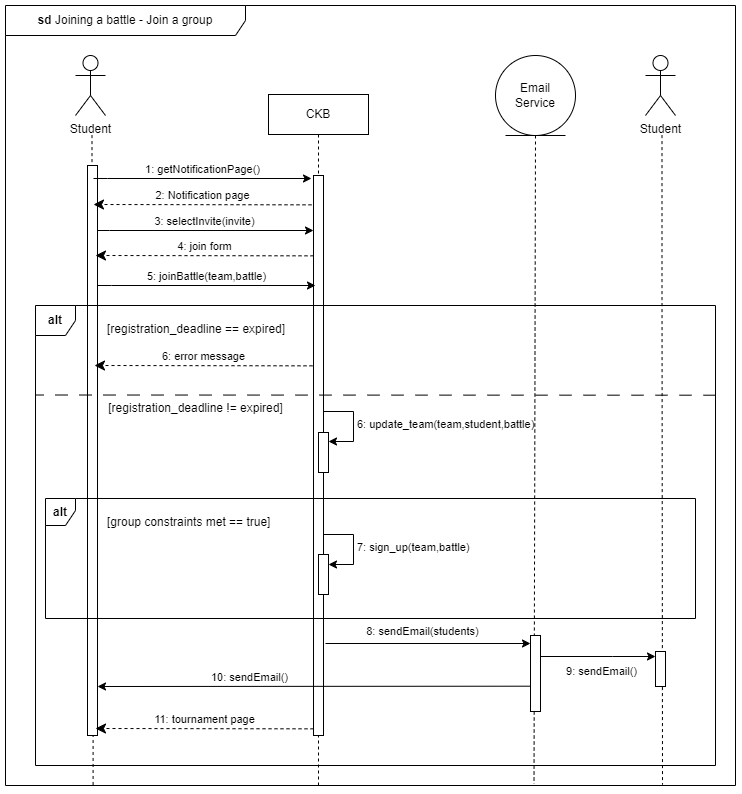
\includegraphics[width=0.95\textwidth]{images/seq_diagrams/joining_battle-join_group.png}
    \caption{Joining a battle by joining a group sequence diagram}
\end{figure}
\clearpage

\begin{figure}[H]
    \centering
    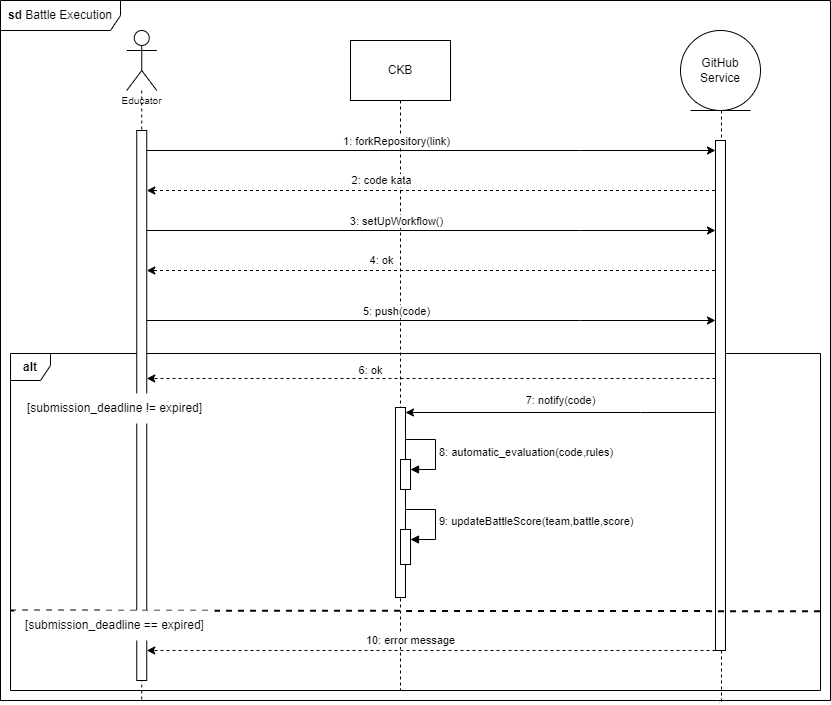
\includegraphics[width=0.95\textwidth]{images/seq_diagrams/battle_execution.png}
    \caption{Joining a battle by joining a group sequence diagram}
\end{figure}
\clearpage

\begin{figure}[H]
    \centering
    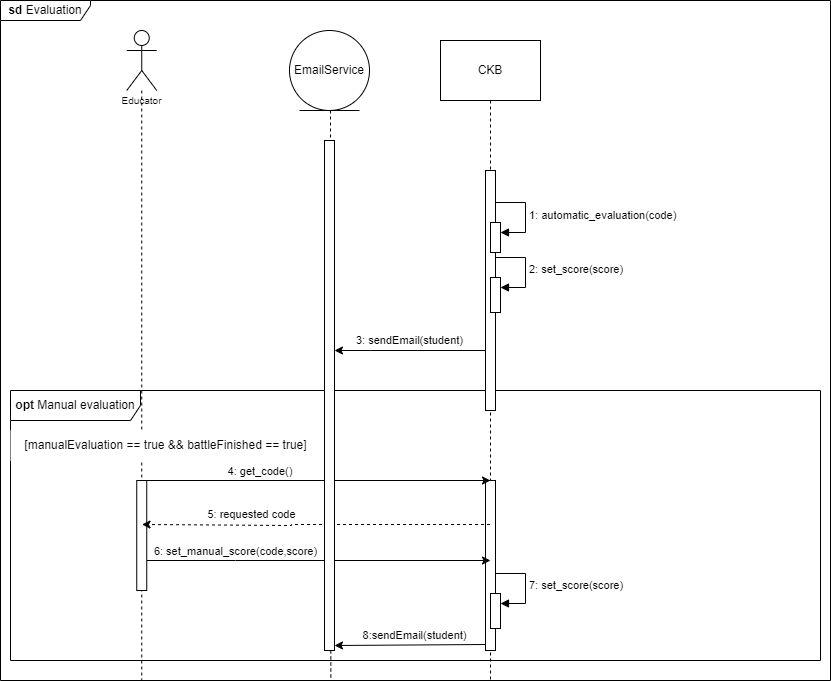
\includegraphics[width=0.95\textwidth]{images/seq_diagrams/Evaluation.png}
    \caption{Evaluation sequence diagram}
\end{figure}
\clearpage

\begin{figure}[H]
    \centering
    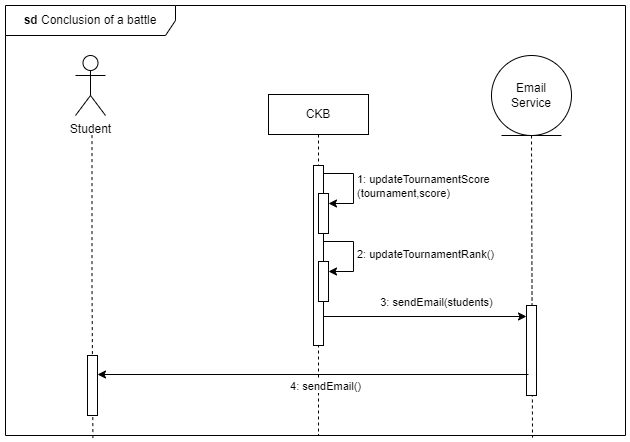
\includegraphics[width=0.95\textwidth]{images/seq_diagrams/battle_conclusion.png}
    \caption{Joining a battle by joining a group sequence diagram}
\end{figure}
\clearpage

\begin{figure}[H]
    \centering
    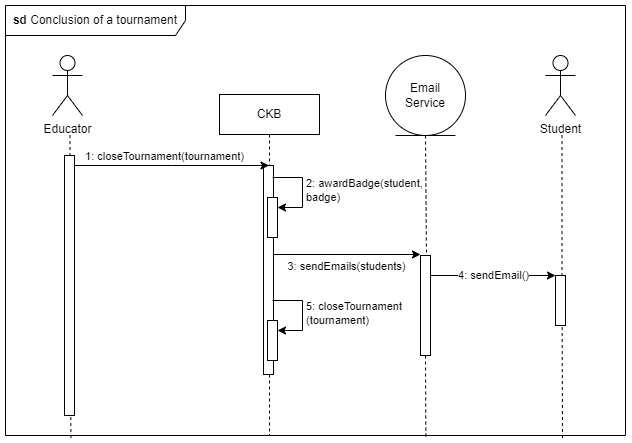
\includegraphics[width=0.95\textwidth]{images/seq_diagrams/tournament_conclusion.png}
    \caption{Joining a battle by joining a group sequence diagram}
\end{figure}
\clearpage


\begin{figure}[H]
    \centering
    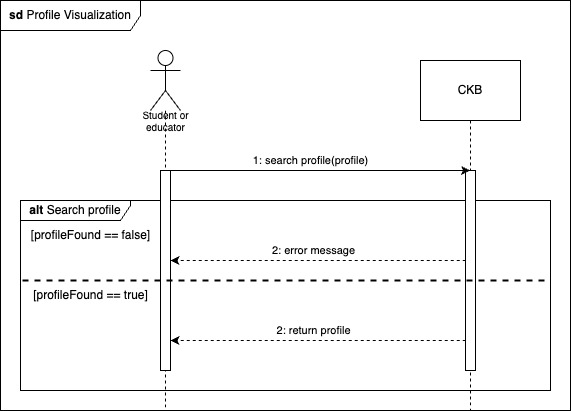
\includegraphics[width=0.9\textwidth]{images/seq_diagrams/profile_visualization.jpg}
    \caption{Profile visualization sequence diagram}
\end{figure}
\clearpage

\subsection{List of functional requirements}
\begin{longtable}{|c|l|}
    \hline
    \rowcolor[HTML]{B8C8D5} 
    {\color[HTML]{000000} \textbf{Requirements}} & \multicolumn{1}{c|}{\cellcolor[HTML]{B8C8D5}{\color[HTML]{000000} \textbf{Description}}} \\ \hline
    \endfirsthead
    %
    \endhead
    %
    R1 \label{R.1}& \begin{tabular}[c]{@{}l@{}}The system must allow the user to register himself to the system \\ by providing all the mandatory information.\end{tabular} \\ \hline
    R2 \label{R.2}& The system must allow the students to link their GitHub account. \\  \hline
    R3 \label{R.3}& \begin{tabular}[c]{@{}l@{}}The system must verify the uniqueness of the email \\ of the user to be registered.\end{tabular} \\ \hline
    R4 \label{R.4}& \begin{tabular}[c]{@{}l@{}}The system must send a confirmation on the user's email after \\ his registration.\end{tabular} \\ \hline
    R5 \label{R.5}& \begin{tabular}[c]{@{}l@{}}The system must allow the user to log into their account by \\ entering their email and password.\end{tabular} \\ \hline
    R6 \label{R.6}& The system must allow educators to create tournaments. \\ \hline
    R7 \label{R.7}& The system must allow the tournament creator to invite other educators. \\ \hline
    R8 \label{R.8}& The systems must allow the tournament creator to end the tournament. \\ \hline
    R9 \label{R.9}& \begin{tabular}[c]{@{}l@{}} The system must allow the tournament creator to set the tournament \\ configuration. \end{tabular}\\ \hline
    R10 \label{R.10}& The system must allow the tournament creator to define badges. \\ \hline
    R11 \label{R.11}& The system must allow students to collect badges. \\ \hline
    R12 \label{R.12}& The system must assign badges to eligible students. \\ \hline
    R13 \label{R.13}& \begin{tabular}[c]{@{}l@{}} The system must notify via email students when a tournament \\ they subscribed to ends. \end{tabular} \\ \hline
    R14 \label{R.14}& The system must notify via email students when they are awarded a badge. \\ \hline
    R15 \label{R.15}& \begin{tabular}[c]{@{}l@{}} The system must notify via email educators when it is time to evaluate \\ students' project. \end{tabular} \\ \hline
    R16 \label{R.16}& \begin{tabular}[c]{@{}l@{}} The system must notify via email educators when they are invited to join \\  a tournament. \end{tabular} \\ \hline
    R17 \label{R.17}& The system must allow authorized educators to create battles. \\ \hline
    R18 \label{R.18}& The system must allow the battle creator to upload the code kata. \\ \hline
    R19 \label{R.19}& The system must allow the battle creator to set the battle configuration. \\ \hline
    R20 \label{R.20}& \begin{tabular}[c]{@{}l@{}} The system must allow the educator to manually evaluate \\ the students' project. \end{tabular} \\ \hline
    R21 \label{R.21}& \begin{tabular}[c]{@{}l@{}} The system must send the link to the repository to all students \\ subscribed to the battle. \end{tabular} \\ \hline
    R22 \label{R.22}& The system must create the GitHub repository containing the code kata.\\ \hline
    R23 \label{R.23}& The system must notify via email students when a new tournament is created. \\ \hline
    R24 \label{R.24}& The system must allow students to join a tournament. \\ \hline
    R25 \label{R.25}& \begin{tabular}[c]{@{}l@{}} The system must notify via email students when a new battle is created \\ within the context of a tournament they signed-up to.\end{tabular} \\ \hline
    R26 \label{R.26}& \begin{tabular}[c]{@{}l@{}} The system must allow students to subscribe to a battle  within \\  the context of a tournament they signed-up to. \end{tabular}\\ \hline
    R27 \label{R.27}& The system must allow students to invite other students to a battle. \\ \hline
    R28 \label{R.28}& \begin{tabular}[c]{@{}l@{}} The system must notify via email students when they are invited to join \\ a battle by another student. \end{tabular} \\ \hline
    R29 \label{R.29}& \begin{tabular}[c]{@{}l@{}} The system must notify vie email students when the final battle rank \\ becomes available. \end{tabular} \\ \hline
    R30 \label{R.30}& \begin{tabular}[c]{@{}l@{}} The system must notify via email students when the final tournament rank \\ becomes available. \end{tabular}\\ \hline
    R31 \label{R.31}& \begin{tabular}[c]{@{}l@{}} The system must pull the latest submitted sources before \\ the submission deadline expired. \end{tabular}\\ \hline
    R32 \label{R.32}& The system must analyze the students' projects. \\ \hline
    R33 \label{R.33}& The system must run the students' projects. \\ \hline
    R34 \label{R.34}& The system must evaluate the students' projects. \\ \hline
    R35 \label{R.35}& The system must update the battle scores of the teams. \\ \hline
    R36 \label{R.36}& The system must compute the battle rank. \\ \hline
    R37 \label{R.37}& The system must update the students' personal tournament scores. \\ \hline
    R38 \label{R.38}& The system must compute the tournament rank. \\ \hline
    R39 \label{R.39}& The system must allow users to visualize ongoing tournaments. \\ \hline
    R40 \label{R.40}& The system must allow users to visualize ongoing tournament ranks. \\ \hline
    R41 \label{R.41}& The system must allow users to visualize students' profiles. \\ \hline
    R42 \label{R.42}& \begin{tabular}[c]{@{}l@{}} The system must notify via email students when their work has \\ been manually evaluated.\end{tabular} \\ \hline
    R43 \label{R.43}& The system must notify via email students when they join a tournament. \\ \hline
\end{longtable}

\subsection{Mapping on requirements}
\begin{table}[H]
    \begin{tabularx}{\textwidth}{X}
        \toprule
        \textbf{G1} Allow students to compete in a tournament                                                       \\ \midrule
        \textbf{Requirements}                                                                                                        \\ \midrule
        \textbf{R1} The system must allow the user to register himself to the system                                                    \\
        \textbf{R2} The system must allow the user to register himself to the system                                         \\ 
        \textbf{R3} The system must verify the uniqueness of the email of the user to be registered                                        \\ 
        \textbf{R4} The system must send a confirmation on the user's email after his registration.                         \\ 
        \textbf{R5} The system must allow the user to log into their account by entering their email and password           \\ 
        \textbf{R11} The system must allow students to collect badges        \\ 
        \textbf{R12} The system must assign badges to eligible students          \\
        \textbf{R13} The system must notify via email students when a tournament they subscribed to ends. \\ 
        \textbf{R17} The system must allow authorized educators to create battles        \\ 
        \textbf{R18} The system must allow the battle creator to upload the code kata       \\ 
        \textbf{R19} The system must allow the battle creator to set the battle configuration                \\ 
        \textbf{R20} The system must allow the educator to manually evaluate the students' project          \\    
        \textbf{R21} The system must send the link to the repository to all students subscribed to the battle            \\ 
        \textbf{R22} The system must create the GitHub repository containing the code kata               \\ 
        \textbf{R23} The system must notify via email students when a new tournament is created            \\ 
        \textbf{R24} The system must allow students to join a tournament     \\ 
        \textbf{R25} The system must notify via email students when a new battle is created within the context of a tournament they signed-up to        \\ 
        \textbf{R26} The system must allow students to subscribe to a battle  within the context of a tournament they signed-up to            \\
        \textbf{R27} The system must allow students to invite other students to a battle     \\ 
        \textbf{R28} The system must notify via email students when they are invited to join \\ a battle by another student        \\ 
        \textbf{R29} The system must notify via email students when the final battle rank becomes available.       \\ 
        \textbf{R30} The system must notify via email students when the final tournament rank becomes available     \\ 
        
    \end{tabularx}
\end{table}

\begin{table}[H]
    \begin{tabularx}{\textwidth}{X}
        \textbf{R31} The system must pull the latest submitted sources before the submission deadline expired     \\  
        \textbf{R35} The system must update the battle scores of the teams       \\ 
        \textbf{R43} The system must notify via email students when they join a tournament. \\
        \textbf{R36} The system must compute the battle rank     \\  
        \textbf{R37} The system must update the students' personal tournament scores         \\ 
        \textbf{R38} The system must compute the tournament rank         \\
        \textbf{R39} The system must allow users to visualize ongoing tournaments    \\
        \textbf{R40} The system must allow users to visualize ongoing tournament ranks       \\
        \textbf{R41} The system must allow users to visualize students' profiles     \\
        \textbf{R42} The system must notify via email students when their work has been manually evaluated. \\
        \midrule
        \textbf{Domain Assumptions}                                                                                                  \\ \midrule
        \textbf{D1} Users provide correct information during the registration process \\
        \textbf{D2} Students have an email and a GitHub account     \\
        \textbf{D3} Users have a stable and reliable Internet connection \\
        \textbf{D4} Students know the functioning of GitHub and GitHub Actions      \\
        \textbf{D5} Educators create at least one battle within a tournament        \\
        \textbf{D6} Students must give consent to access their GitHub account       \\
        \textbf{D7} Educators upload a correct code kata        \\
        \bottomrule
    \end{tabularx}
\end{table}

\begin{table}[H]
    \begin{tabularx}{\textwidth}{X}
        \toprule
        \textbf{G2} Allows educators to create challenges for students.                                                    \\ \midrule
        \textbf{Requirements}                                                                                                        \\ \midrule
        \textbf{R1} The system must allow the user to register himself to the system                                                   \\
        \textbf{R3} The system must verify the uniqueness of the mail of the user to be registered                                       \\ 
        \textbf{R4} The system must send a confirmation on the user's email after his registration.                         \\ 
        \textbf{R5} The system must allow the user to log into their account by entering their email and password           \\
        \textbf{R6} The system must allow educators to create tournaments.              \\ 
        \textbf{R7} The system must allow the tournament creator to invite other educators.         \\ 
        \textbf{R8} The systems must allow the tournament creator to end the tournament     \\ 
        \textbf{R9} The system must allow the tournament creator to set the tournament configuration          \\ 
        \textbf{R10} The system must allow the tournament creator to define badges.      \\ 
        \textbf{R11} The system must allow students to collect badges        \\ 
        \textbf{R12} The system must assign badges to eligible students          \\  
        \textbf{R14} The system must notify via email students when they are awarded a badge. \\ 
        \textbf{R15} The system must notify via email educators when it is time to evaluate students' project      \\ 
        \textbf{R16} The system must notify via email educators when they are invited to join a tournament      \\
        \textbf{R17} The system must allow authorized educators to create battles        \\ 
        \textbf{R18} The system must allow the battle creator to upload the code kata       \\
        \textbf{R19} The system must allow the battle creator to set the battle configuration       \\ 
        \textbf{R23} The system must notify via email students when a new tournament is created            \\
        \textbf{R41} The system must allow users to visualize students' profiles     \\
        \midrule
        \textbf{Domain Assumptions}                                                                                                  \\ \midrule
        \textbf{D1} Users provide correct information during the registration process \\   
        \textbf{D3} Users have a stable and reliable Internet connection \\
        \textbf{D5} Educators create at least one battle within a tournament        \\
        \textbf{D7} Educators have a good knowledge of programming      \\
        \textbf{D8} Educators upload a correct code kata        \\
        \bottomrule
    \end{tabularx}
\end{table}

\begin{table}[H]
    \begin{tabularx}{\textwidth}{X}
        \toprule
        \textbf{G3} Allows educators to grade students' projects.                                                    \\ \midrule
        \textbf{Requirements}                                                                                                        \\ \midrule
        \textbf{R1} The system must allow the user to register himself to the system                                                     \\
        \textbf{R3} The system must verify the uniqueness of the email of the user to be registered                                       \\ 
        \textbf{R4} The system must send a confirmation on the user's email after his registration                         \\
        \textbf{R5} The system must allow the user to log into their account by entering their email and password           \\
        \textbf{R6} The system must allow educators to create tournaments.              \\
        \textbf{R7} The system must allow the tournament creator to invite other educators.         \\  
        \textbf{R20} The system must allow the educator to manually evaluate the students' project.          \\ 
        \textbf{R31} The system must pull the latest submitted sources before the submission deadline expired     \\ 
        \textbf{R32} The system must analyze the students' projects      \\ 
        \textbf{R33} The system must run the students' projects      \\
        \textbf{R34} The system must evaluate the students' projects     \\ 
        \textbf{R38} The system must compute the tournament rank                 \\ 
        \textbf{R42} The system must notify via email students when their work has been manually evaluated. \\
        \midrule
        \textbf{Domain Assumptions}                                                                                                  \\ \midrule
        \textbf{D1} Users provide correct information during the registration process \\           
        \textbf{D2} Students have an email and a GitHub account     \\
        \textbf{D3} Users have a stable and reliable Internet connection \\
        \textbf{D5} Educators create at least one battle within a tournament        \\
        \textbf{D7} Educators have a good knowledge of programming      \\
        \bottomrule
    \end{tabularx}
\end{table}

\begin{table}[H]
    \begin{tabularx}{\textwidth}{X}
        \toprule
        \textbf{G4} Allows students to collect badges in a tournament proving their skills.                                       \\ \midrule
        \textbf{Requirements}                                                                                                        \\ \midrule
        \textbf{R1} The system must allow the user to register himself to the system                                                  \\
        \textbf{R2} The system must allow the user to register himself to the system                                               \\ 
        \textbf{R3} The system must verify the uniqueness of the email of the user to be registered                                        \\ 
        \textbf{R4} The system must send a confirmation on the user's email after his registration.                         \\ 
        \textbf{R5} The system must allow the user to log into their account by entering their email and password           \\ 
        \textbf{R10} The system must allow the tournament creator to define badges.      \\ 
        \textbf{R11} The system must allow students to collect badges        \\ 
        \textbf{R12} The system must assign badges to eligible students          \\  
        \textbf{R14} The system must notify via email students when they are awarded a badge. \\ 
        \textbf{R31} The system must pull the latest submitted sources before the submission deadline expired     \\ 
        \textbf{R32} The system must analyze the students' projects      \\ 
        \textbf{R38} The system must compute the tournament rank                 \\ 
        \midrule
        \textbf{Domain Assumptions}                                                                                                  \\ \midrule
        \textbf{D1} Users provide correct information during the registration process \\          
        \textbf{D3} Users have a stable and reliable Internet connection \\
        \bottomrule
    \end{tabularx}
\end{table}

\clearpage
\subsection{Mapping on use cases}
\begin{table}[H]
    \begin{tabularx}{\textwidth}{XXX}
        \toprule
        \textbf{Use Case}                     & \textbf{Requirements} \\ \midrule
        UC1 - Login                           & R5                   \\
        UC2 - Registration                    & R1 R2 R3 R4               \\
        UC3 - Tournament creation             & R6 R7 R9 R10 R16 R23  \\
        UC4 - Battle creation                 & R17 R18 R19 R21 R25       \\
        UC5 - Tournament visualization        & R39 R40          \\
        UC6 - Joining a tournament            & R24 R43        \\
        UC7 - Joining a battle                & R26 R27 R28      \\
        UC8 - Battle execution                & R22              \\
        UC9 - Evaluation                      & R15 R20 R31 R32 R33 R34 R42     \\
        UC10 - Conclusion of a battle         & R29 R35 R36 R37 R38         \\
        UC11 - Conclusion of a tournament     & R8 R11 R12 R13 R14 R30              \\
        UC12 - Profile visualization          & R41              \\
        \bottomrule
    \end{tabularx}
\end{table}

\clearpage
\section{Performance Requirements}
This section presents the performance requirements which need to be fulfilled to make the
whole system as usable as possible.\\
To provide the best user experience, the system must be able to provide a scalable, reactive 
and capable of load-balancing backend, assure protection against DDoS attacks and provide a 
responsive and fluid frontend.\\
The frontend must handle correctly asynchronous interactions with the server, even when the 
connection quality is bad, in order to provide the best possible experience.\\

\section{Design Constraints}

\subsection{Standards compliance}
Specifications described in this document must be respected by the system. Source code of the application
must be commented on and documented adequately. The system should respect the guidelines described
by the GDPR.\\

\subsection{Hardware limitations}
The system requires a computer with a web browser and a stable internet connection.\\

%\subsection{Any other constraint}

\section{Software System Attributes}

\subsection{Reliability}
In order to guarantee better reliability performances, all the scheduled maintenance of the system should
be done during the night. Some functionalities of the system rely on external APIs, though the system should 
not completely fail because of failures in one of those. It is also critical to avoid data loss through 
redundant storage methods.

\subsection{Availability}
The system should offer its functionalities with an availability equal to 99.7\%. This means that, on average, 
the system must be inaccessible for at most one day every year. To achieve this goal, the system should 
provide a high redundancy for the most critical components.

\subsection{Security}
To protect users sensible data the system must collect the minimum data possible, and store them in an
encrypted database. The connection between the application must follows modern standard secure protocols as
HTTPS. Not only passwords should be considered as sensible data, but also users' email addresses and GitHub accounts. 
All passwords must be salted and hashed.

\subsection{Maintainability}
The system should be designed to be easily maintainable. This means that the code should be well documented 
and commented, and the architecture should be modular and well designed.

\subsection{Portability}
The application must run on any OS (Windows, Linux, MacOS) that supports a web browser.
	\chapter{Formal Analysis}

	\chapter{Effort Spent}
\subsection*{Group working}
\begin{table}[H]
    \begin{tabular}{lr}
        \toprule
        \textbf{Project Specification Analysis, Brainstorming, RASD structure} & \textbf{4h} \\
        \textbf{Study of the context and existing protocols}                   & \textbf{3h} \\
        \textbf{Goals and Phenomena elicitation}                               & \textbf{5h} \\
        \textbf{Use cases diagrams and description}                            & \textbf{7h} \\
        \textbf{Definitions, Acronyms}                                         & \textbf{1h} \\
        \textbf{Assumptions, dependencies, constraints}                        & \textbf{2h} \\
        \textbf{List of functional requirements}                               & \textbf{2h} \\
        \textbf{Formal Analysis with Alloy}                                    & \textbf{4h} \\
        \textbf{Scenarios}                                                     & \textbf{3h} \\
        \textbf{Final Review}                                                  & \textbf{4h} \\
        \bottomrule
    \end{tabular}
\end{table}

\subsection*{Chiara}
\begin{table}[H]
    \begin{tabular}{lr}
        \toprule
        \textbf{Sequence diagrams}                                             & \textbf{4h} \\
        \textbf{Class Diagram}                                                 & \textbf{2h}  \\
        \textbf{UML}                                                           & \textbf{3h}  \\
        \textbf{User characteristics}                                          & \textbf{1h}  \\
        \textbf{Mapping on use cases}                                          & \textbf{2h}   \\
        \bottomrule
    \end{tabular}
\end{table}

\subsection*{Flavia}
\begin{table}[H]
    \begin{tabular}{lr}
        \toprule
        \textbf{User Interfaces} & \textbf{6h}  \\
        \textbf{State Diagrams}  & \textbf{2h} \\
        \textbf{Mapping on goals, on requirements} & \textbf{3h}   \\
        \bottomrule
    \end{tabular}
\end{table}

\subsection*{Gianluca}
\begin{table}[H]
    \begin{tabular}{lr}
        \toprule
        \textbf{Sequence diagrams}                                             & \textbf{4h} \\
        \textbf{Formal Analysis with Alloy}                                    & \textbf{4h}  \\
        \textbf{Product Functions}                                             & \textbf{2h} \\
        \textbf{Hardware Interfaces, Software Interfaces, Communication Interfaces}   & \textbf{2h}   \\
        \textbf{Software system attributes}                                    & \textbf{1h}   \\
        \bottomrule
    \end{tabular}
\end{table}
	\chapter{References}
\begin{itemize}
    \item Software Engineering II course slides
    \item Use Case Diagrams and Sequence Diagrams were made using draw.io\\ \url{https://app.diagrams.net/}
    \item Alloy Analyzer\\ \url{https://github.com/AlloyTools/org.alloytools.alloy}
    \item UI Mockup \\ \url{https://www.figma.com/}
\end{itemize}
\end{document}